
\chapter{Quark Gluon Analysis}
\label{ch:quark_gluon_analysis}

\newthought{As any dedicated reader} can clearly see, the Ideal of practical reason is a representation of, as far as I know, the things in themselves; as I have shown elsewhere, the phenomena should only be used as a canon for our understanding. The paralogisms of practical reason are what first give rise to the architectonic of practical reason. As will easily be shown in the next section, reason would thereby be made to contradict, in view of these considerations, the Ideal of practical reason, yet the manifold depends on the phenomena.


\section{Data Preprocessing}
\label{sec:q:data_preprocessing}

The data consists of \num{43} data files taken between \num{1991} and \num{1995} totalling \SI{3.5}{\giga\byte} (Data). Along with this comes \num{125} files based on Monte Carlo (MC) simulations (\SI{8.4}{\giga\byte}) and additional \num{42} MC-files with only $b$-quark events (MCb) simulated (\SI{2.1}{\giga\byte}). The data files which are in the form of \emph{Ntuples}, ROOT's data format \autocite{brunROOTObjectOriented1997}, are converted to HDF5-files by using uproot \autocite{ScikithepUproot2019}. While iterating over the Ntuples, some basic cuts are applied before exporting the data to HDF5. The first one being that the (center of mass) energy $E$ in the event has to be within $\SI{90.8}{\GeV} \leq E \leq \SI{91.6}{\GeV}$ to only use the $Z$ peak data. The second one being that the sum of the momenta $p_\mathrm{sum}$ in each event is $\SI{32}{\GeV} \leq p_\mathrm{sum}$ to remove any $Z \rightarrow \tau^+ \tau^-$ events. To ensure a primary vertex, at least two good tracks are required where a good track is defined as having \num{7} TPC hits and $\geq$ 1 silicon hit. Finally it is required that the cosine of the thrust axis polar angle, which is the angle between the trust axis and the beam, is less than or equal to \num{0.8} to avoid any low angle events since the detector performance worsens significantly in that region. These cuts were standard requirements for the ALEPH experiment.
% (P. Hansen, personal communication, December, 2019, XXX).

One last cut which was experimented with was the threshold value for \emph{jet matching}. The jet matching is the process of matching the jet with one of the final state quarks. The jet is said to be matched if the dot product of between the final quark momentum and the jet momentum is more than then threshold value. Higher thresholds means cleaner jets but at the expense of less statistics. A jet matching threshold of \num{0.90} was found to be a good compromise between purity and quantity where \SI{97.8}{\percent} of all 2-jet events are matched and \SI{96.7}{\percent} of all other jets were matched\sidenote{Compare this to \SI{98.5}{\percent} and \SI{97.8}{\percent} for a threshold of \num{0.85} or \SI{95.9}{\percent} and \SI{93.9}{\percent} for a threshold of \num{0.95}.}.  

The data structure is quite differently structured in the Ntuples compared to normal structured data in the form of tidy data \autocite{JSSv059i10}. The data is organized such that one iterates over each event where the variables are variable-length depending on the number of jets in the events; this is also known as \emph{jagged} arrays. The data is un-jagged\sidenote{Such that e.g. a 3-jet event will figure as three rows in the dataset.} before exporting to HDF5-format and only the needed variables are kept. This reduces the total output file to a \SI{2.9}{\giga\byte} HDF5-file for both Data, MC, and MCb.

The number of events for each number of jets can be seen in Table~\ref{tab:q:datasize_data} for the Data and in Figure~\ref{tab:q:datasize_MC} for the MC and MCb. 

\begin{margintable}
  \centering
  \begin{tabular}{@{}rrr@{}}
  {} &       jets &     events \\
  \midrule
  \num{2}     &  \num{2359738} &  \num{1179869} \\
  \num{3}     &  \num{3619290} &  \num{1206430} \\
  \num{4}     &   \num{854336} &   \num{213584} \\
  \num{5}     &    \num{52775} &    \num{10555} \\
  \num{6}     &      \num{510} &       \num{85} \\
  Total       &  \num{6886649} &  \num{2610523} \\  
  \end{tabular}
  \vspace{\abovecaptionskip}
  \caption[Dimensions of dataset for Data]{The dimensions of the dataset for the actual Data. The numbers in the jet columns are the number of events multiplied with the number of jets; e.g. $85 \cdot 6 = 510$.}
  \label{tab:q:datasize_data}
\end{margintable}

\begin{margintable}
  \centering
  \begin{tabular}{@{}rrr@{}}
  {} &       jets &     events \\
  \midrule
  \num{2}     &  \num{7293594} &  \num{3646797} \\
  \num{3}     &  \num{10780890} &  \num{3593630} \\
  \num{4}     &   \num{2241908} &   \num{560477} \\
  \num{5}     &    \num{103820} &    \num{20764} \\
  \num{6}     &      \num{588} &       \num{98} \\
  Total       &  \num{20420800} &  \num{7821766} \\  
  \end{tabular}
  \vspace{\abovecaptionskip}
  \caption[Dimensions of dataset for MC and MCb]{The dimensions for the MC and MCb datasets.}
  \label{tab:q:datasize_MC}
\end{margintable}

\FloatBarrier
\section{Explanatory Data Analysis} \label{sec:q:EDA}

Since the machine learning models are only trained on the three vertex variables \code{projet}, \code{bqvjet}, and \code{ptljet} -- see \autoref{ch:hep:particle_physcis_LEP} for a deeper introduction to these variables -- these variables will be the primary focus of this section. Given the fact that MC-simulated data exists, the truth of each simulated event is also known. This allows us visualize the difference between the different types of quarks. In the MC simulation each event are generated such that the type of quark, or \emph{flavor}, is known and assigned the variable \code{flevt}. The mapping from flavor to \code{flevt} is:
\begin{table}[h!]
  \centering
  \begin{tabular}{@{}rccccc@{}}
  Flavor: & $bb$ & $cc$ & $ss$ & $dd$ & $uu$  \\
  % \midrule
  \code{flevt}: & \num{5} & \num{4} & \num{3} & \num{2} & \num{1}  
  \end{tabular}
  \vspace{\abovecaptionskip}
  % \caption{The dimensions for the MC and MCb datasets.}
  % \label{tab:q:flevt}
\end{table}

In addition to knowing the correct flavor, we define that an event is \emph{$q$-matched} if one, and only one, of the jets are assigned to one of the quarks, one, and only one, of the jets are assigned to the other quark, and no other jets are matched to any of the quarks. We can then define what constitutes a $b$-jet: if it has \code{flevt} $= 5$, the entire event is $q$-matched, and the jet is matched to one of the quarks. Similarly we define $c$-jets only with the change that \code{flevt} $= 5$, and $uds$-jets with \code{flevt} $\in \{1, 2, 3\}$. A gluon jet is defined as an any-flavor event which is $q$-matched but the jet is not assigned to any of the quarks. Strictly speaking, this means that $g$-jet is not \SI{100}{\percent} certain of being a gluon, however, since the MC simulation does not contain this information this is the only option. Due to the $q$-match criterion this also means that some jets are assigned the label \q{non-$q$-matched} which is regarded as background. The distribution of different types of jets can be seen in Table~\ref{tab:q:flevt_overview} and shown as relative numbers in Table~\ref{tab:q:flevt_overview_percent_relative} in the appendix.

\begin{table}[h!]
  \centering
  \begin{tabular}{@{}rrrrrr@{}}
    {}    & \multicolumn{1}{c}{$b$} & \multicolumn{1}{c}{$c$} & \multicolumn{1}{c}{$uds$} & \multicolumn{1}{c}{$g$} & non-$q$-matched    \\ 
    \midrule
    2     & \num{2713454} &  \num{944380} & \num{2125900} &       \num{0} & \num{1509860} \\
    3     & \num{2433878} &  \num{964212} & \num{2129218} & \num{3365969} & \num{1887613} \\
    4     &  \num{326264} &  \num{156332} &  \num{336548} & \num{1012198} &  \num{410566} \\
    5     &   \num{10332} &    \num{5960} &   \num{12668} &   \num{54525} &   \num{20335} \\
    6     &      \num{42} &      \num{26} &      \num{52} &     \num{320} &     \num{148} \\
    \midrule
    Total & \num{5483970} & \num{2070910} & \num{4433012} & \num{4604386} & \num{3828522} \\
  \end{tabular}
  \caption{Number of different types of jets for MC and MCb. See also Table~\ref{tab:q:flevt_overview_percent_relative} in the appendix for relative numbers.}
  \label{tab:q:flevt_overview}
\end{table}

With the criteria defined above for what constitutes a specific type of jet the 1D-distributions for the three vertex variables is plotted in Figure~\ref{fig:q:vertex_variables}. For all three subplots the histograms are show with a logarithmic $y$-axis, all $b$-jets in blue, $c$-jets in red, $g$-jets in green and all jets in orange. In fully opaque color are shown the distributions for 2-jet events, in dashed (and lighter color) 3-jet events, and in semi-transparent 4-jet events. In the left subplot the \code{projet} variable is plotted where it can be seen that high values of \code{projet} tend to indicate $b$-jets. In the middle subplot \code{bqvjet} is plotted which shares many similarities with the \code{projet}-variables, including that high values indicate $b$-jets. In the right subplot the \code{ptljet} is plotted. This variable has many zeros in it which correlates with mostly with gluon\sidenote{Around \SI{98}{\percent} of all $g$-jets are zeros compared to $\sim \SI{82}{\percent}$ for $c$-jets and $\sim \SI{70}{\percent}$ for $b$-jets.} and large values are mostly due to $b$-jets. In general it is clear to se how the differences in distribution between the \num{2}-, \num{3}-, and \num{4}-jet events are minor, with the one exception of \num{2}-jet events which does not contain any gluons at all. 

\begin{figure}
  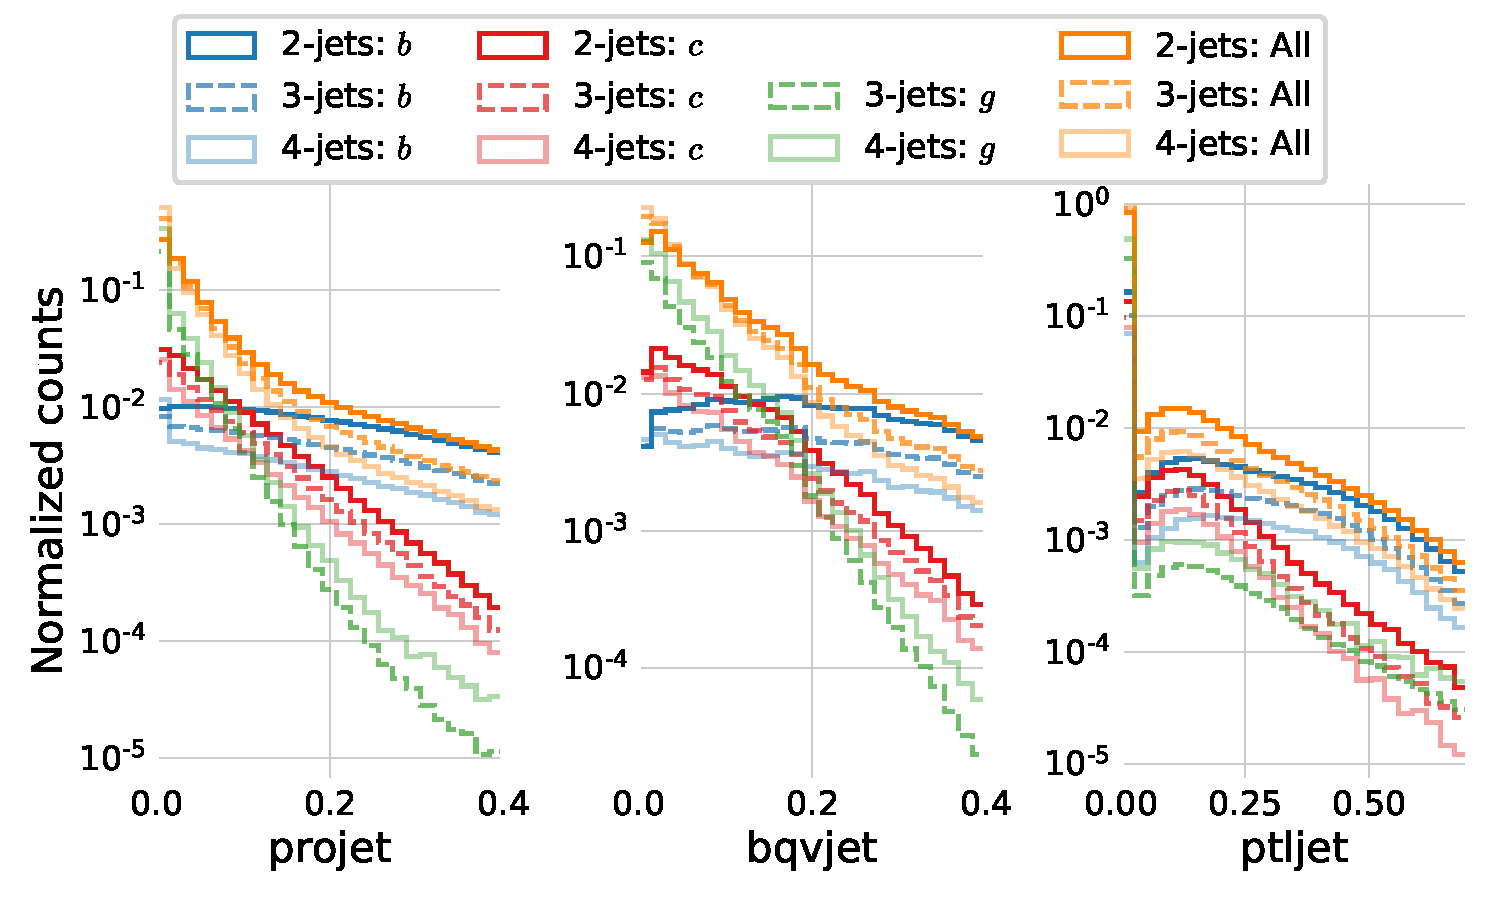
\includegraphics[width=0.98\textwidth, trim=0 0 0 0, clip]{figures/quarks/btagging_variables_hist-down_sample=1.00-ML_vars=vertex-selection=b-ejet_min=4-n_iter_RS_lgb=99-n_iter_RS_xgb=9-cdot_cut=0.90-version=19.pdf}
  \caption[Histograms of the vertex variables]
          {Normalized histograms of the three vertex variables: \code{projet}, \code{bqvjet}, and \code{ptljet}. In blue colors the variables are shown for \textcolor{blue}{true b-jets}, in red for \textcolor{red}{true c-jets}, in green for \textcolor{green}{true g-jets}, and in orange for \textcolor{orange}{all of the jets} (including non q-matched). In fully opaque color are shown the distributions for 2-jet events, in dashed (and lighter color) 3-jet events, and in semi-transparent 4-jet events. Notice the logarithmic y-axis, that there are no g-jets for 2-jet events (as expected), and that all of the distributions are very similar not matter how many jets.
          } 
  \label{fig:q:vertex_variables}
\end{figure}

Even though there are only three vertex variables, it is difficult to properly get an intuition about how easily separated they different types of jets are. Since there are millions of points a single 3D scatter plot quickly becomes overcrowded in one wants to plot all jets. We apply dimensionality reduction from the three dimensions down to two dimensions by using the UMAP algorithm \autocite{mcinnesUMAPUniformManifold2018}. Within recent years the field of dimensionality reduction algorithms has grown a lot from just the typical (linear) principal component analysis to also include non-linear algorithms. The t-SNE algorithm \autocite{maatenVisualizingDataUsing2008} deserves an honorable mention since this algorithm revolutionized the usage of (nonlinear) dimensionality reduction algorithms in e.g. bioinformatics \citep{toghieshghiQuantitativeComparisonConventional2019, wallachProteinSmallmoleculeDatabase2009}  yet its mathematical foundation has strongly been improved with the never, faster UMAP algorithm \autocite{mcinnesUMAPUniformManifold2018} which usage is also expanding \citep{bechtEvaluationUMAPAlternative2018, bechtDimensionalityReductionVisualizing2019, diaz-papkovichUMAPRevealsCryptic2019}.

The aim of UMAP, short for Uniform Manifold Approximation and Projection, is to correctly identify and preserve the structure, or topology, of the high-dimensional feature space in a lower-dimensional output space. It does so by trying to stitch together local manifolds in the high-dimensional feature space such that the difference between the high- and low-dimensional representations is minimized according to the cross-entropy such that both global structure and local structure is preserved \citep{mcinnesUMAPUniformManifold2018}. Compared to t-SNE the approach in UMAP has an algebraic topological background compared to the more heuristic approach taken by t-SNE. Note that the UMAP algorithm is not provided any information about which jets are which types. 

\begin{marginfigure}
  \centerfloat
  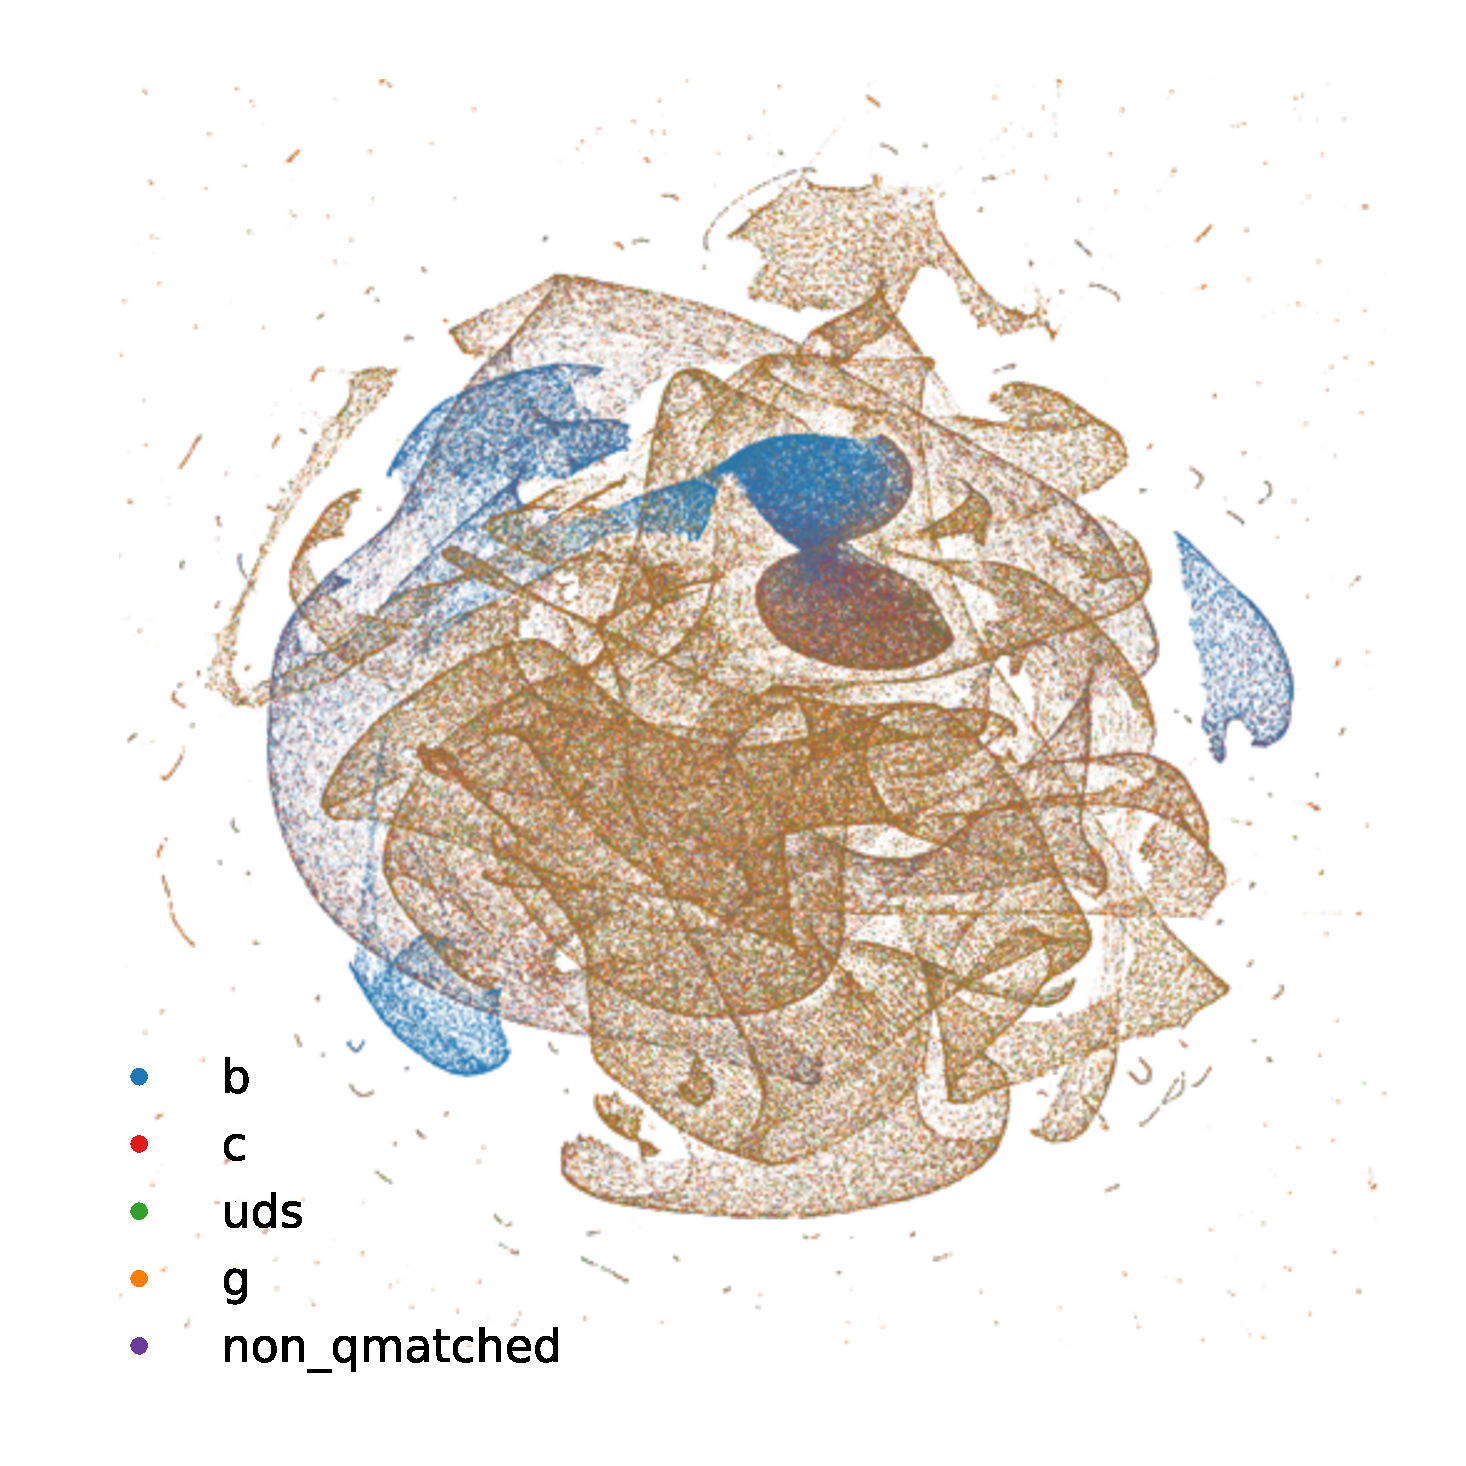
\includegraphics[draft=true, width=0.95\textwidth, trim=50 45 50 50, clip]{figures/quarks/df_UMAP-X=1120952-n_neighbors=250-min_dist=0.2-metric=euclidean-input2b_njet=4_algorithm=UMAP_single.pdf}
  \caption[UMAP visualization of vertex variables for 4-jet events]
          {Visualization of the vertex variables for the different categories: \textcolor{blue}{true b-jets} in blue, \textcolor{red}{true c-jets} in red, \textcolor{green}{true uds-jets} in green, \textcolor{orange}{true g-jets} in orange, and \textcolor{purple}{non q-matched} events in purple. The clustering is performed with the UMAP algorithm which outputs a 2D-projection. This projection is then visualized using the Datashader which takes takes care of point size, avoids over and underplotting, and color intensity.} 
  \label{fig:q:UMAP_vertex_2j}
\end{marginfigure}

\begin{marginfigure}
  \centerfloat
  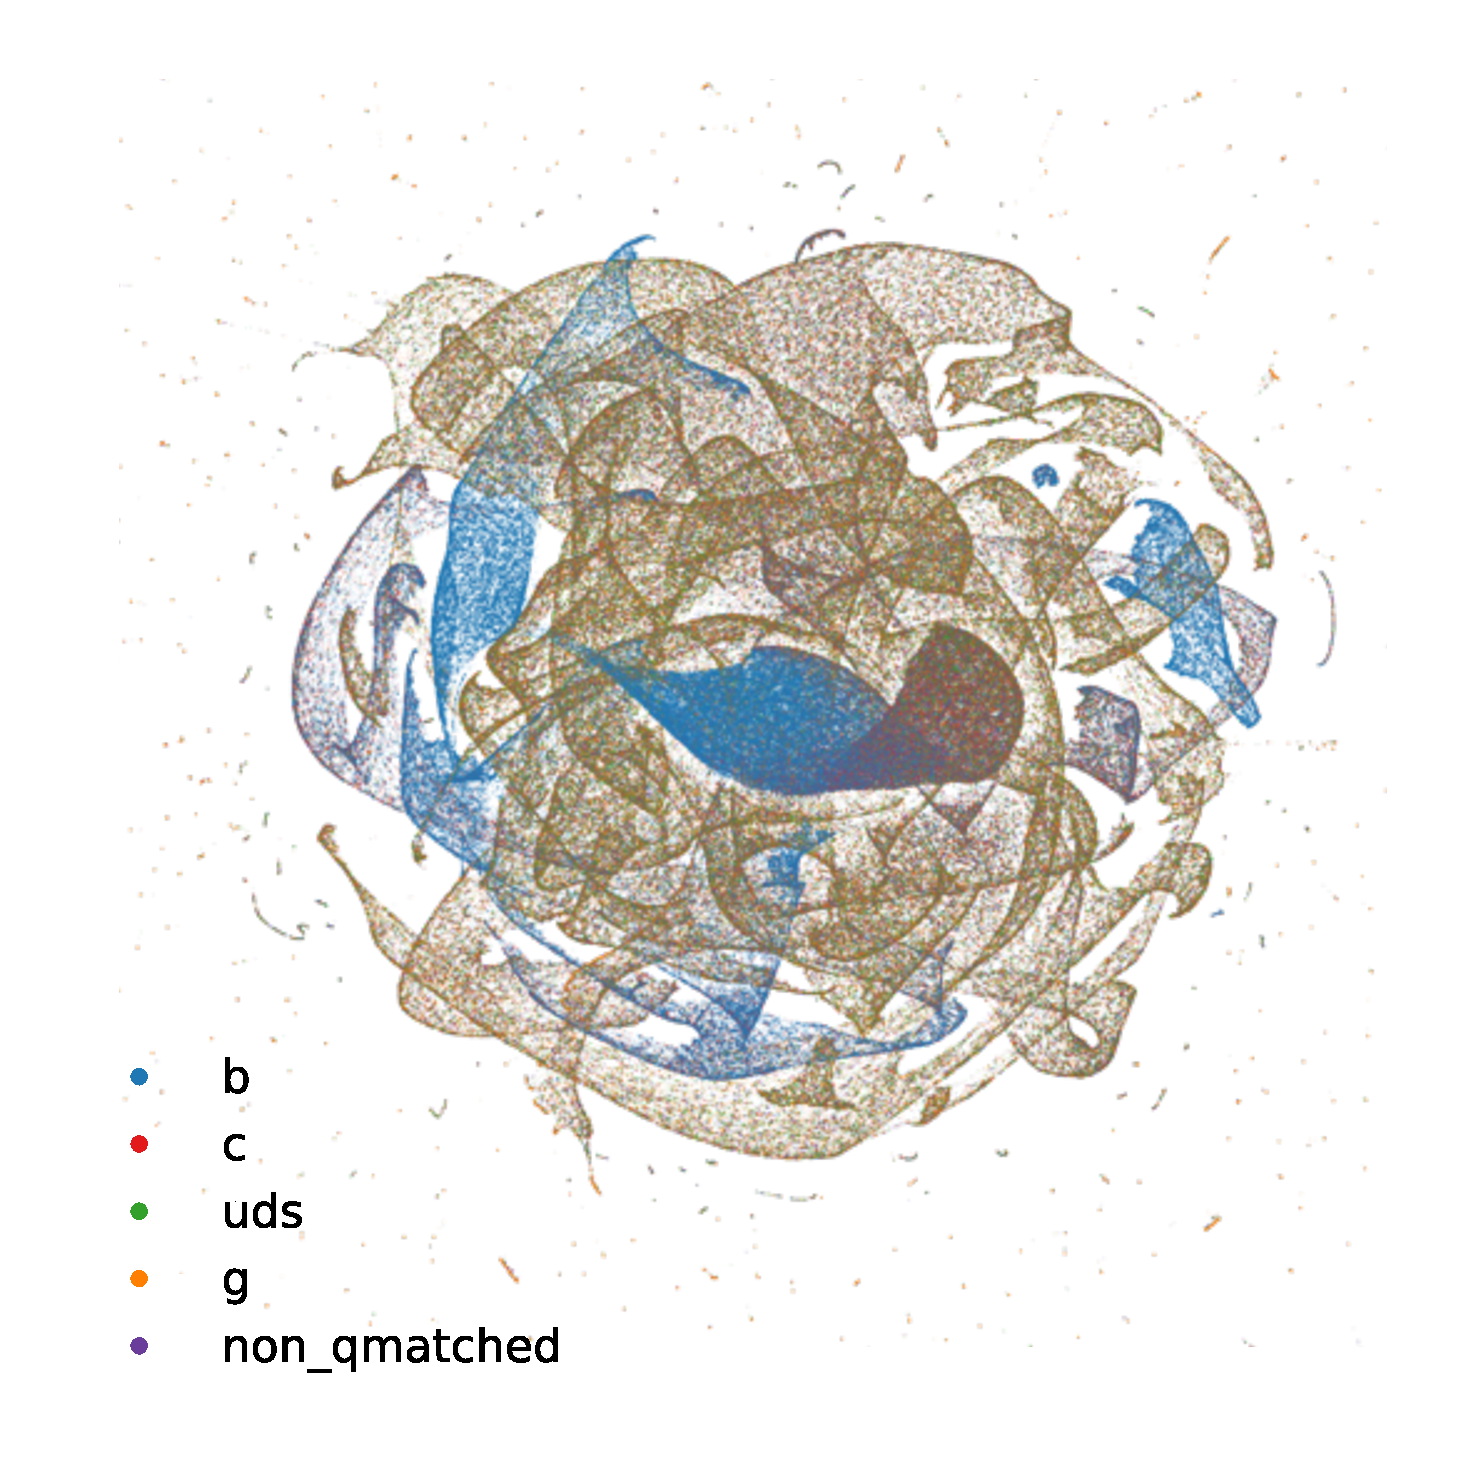
\includegraphics[draft=true, width=0.95\textwidth, trim=50 45 50 50, clip]{figures/quarks/df_UMAP-X=1078089-n_neighbors=250-min_dist=0.2-metric=euclidean-input2b_njet=3_algorithm=UMAP_single.pdf}
  \caption[UMAP visualization of vertex variables for 3-jet events]
          {UMAP visualization of vertex variables for 3-jet events.} 
  \label{fig:q:UMAP_vertex_3j}
\end{marginfigure}

\begin{marginfigure}
  \centerfloat
  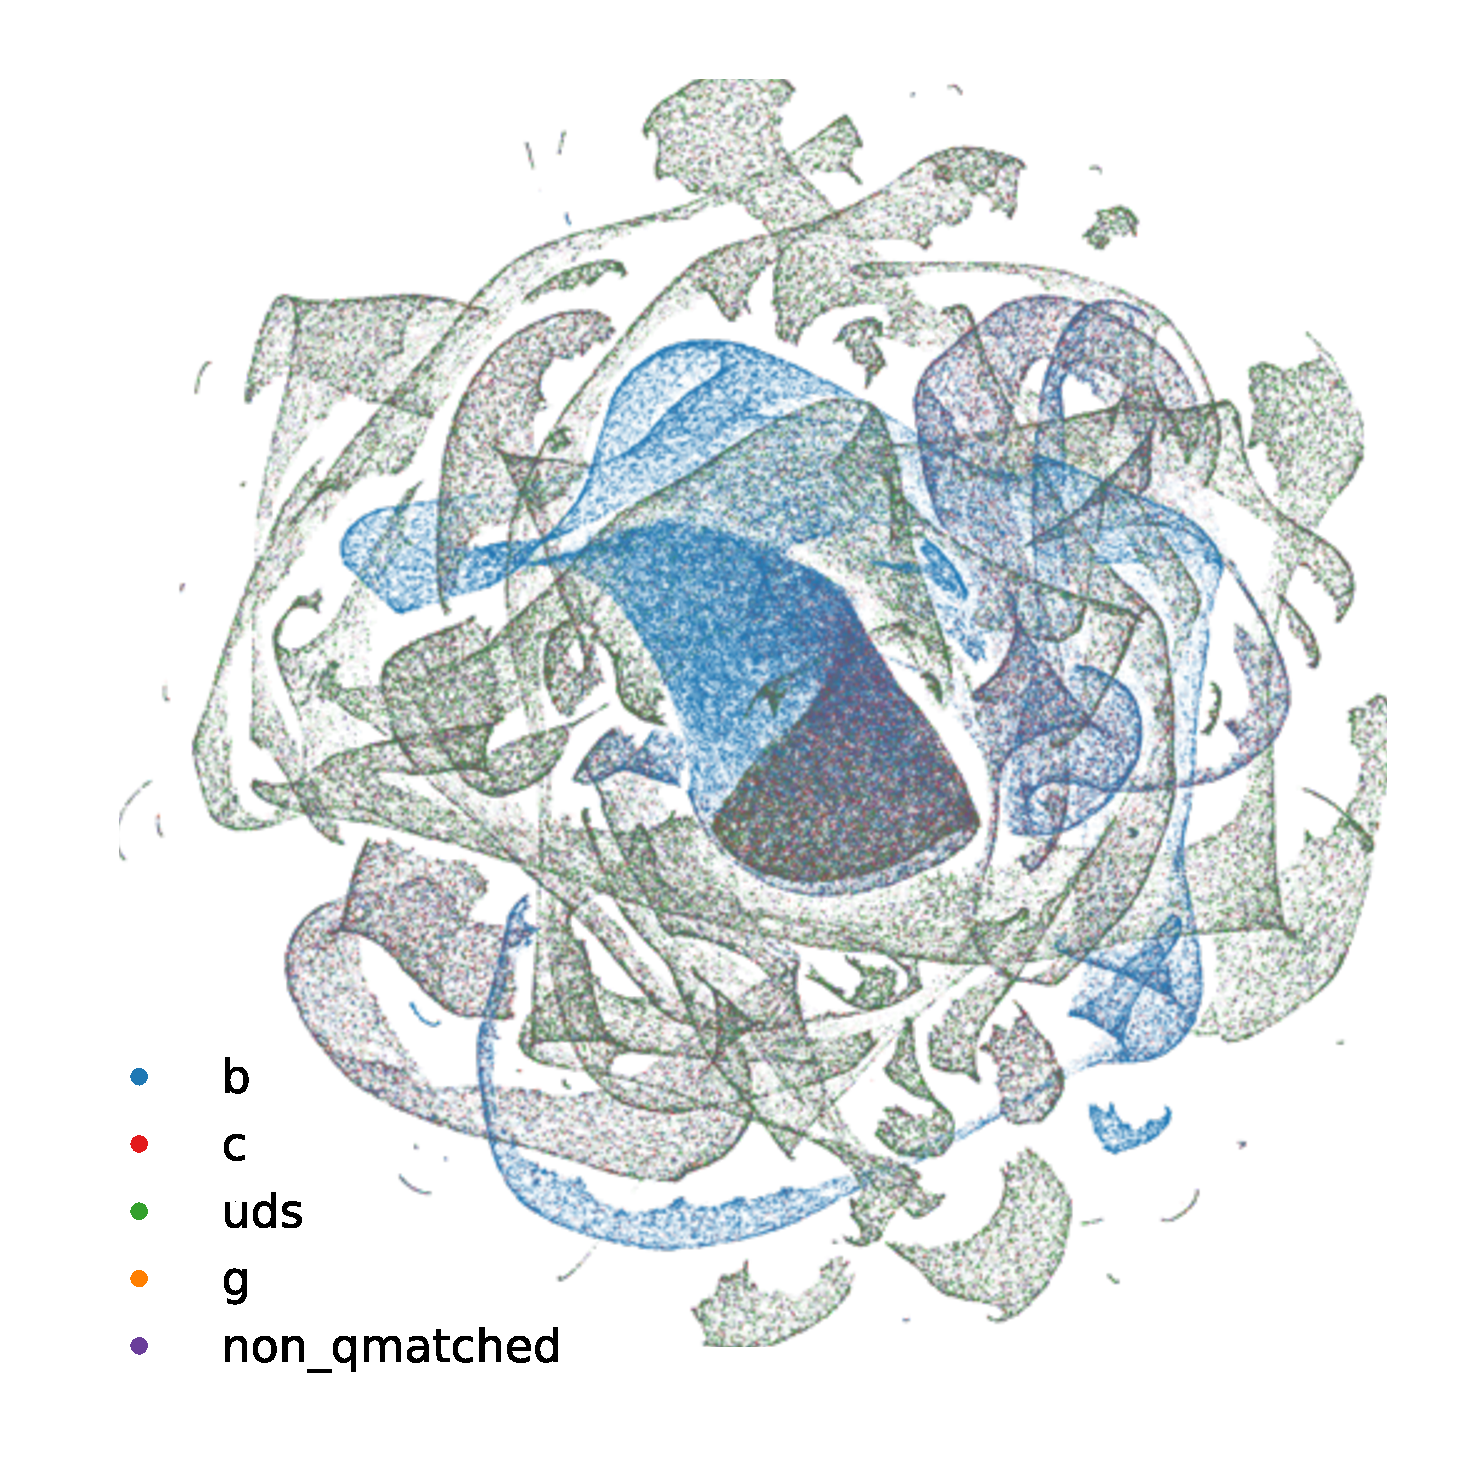
\includegraphics[draft=true, width=0.95\textwidth, trim=50 45 50 50, clip]{figures/quarks/df_UMAP-X=729358-n_neighbors=250-min_dist=0.2-metric=euclidean-input2b_njet=2_algorithm=UMAP_single.pdf}
  \caption[UMAP visualization of vertex variables for 2-jet events]
          {UMAP visualization of vertex variables for 2-jet events.} 
  \label{fig:q:UMAP_vertex_2j}
\end{marginfigure}

The UMAP algorithm has several hyperparameters, where two of the most important ones are the number of neighbors \code{n_neighbors} which controls the priority between correctly preserving the global versus the local structure, and the \code{min_dist} which defines how tightly together UMAP is allowed to cluster the points in the low-dimensional representation. To properly choose the best combination of \code{n_neighbors} and \code{min_dist} a grid search with \code{n_neighbors}~$\in \{10, 50, 100, 250 \}$ and \code{min_dist}~$\in \{0, 0.2, 0.5\}$ is performed. This is shown for 4-jet events in Figure~\ref{fig:q:UMAP_vertex_all} in the appendix. In this case the choice of best combination of \code{n_neighbors} and \code{min_dist} is subjective at best, but it was judged by the author that \code{n_neighbors}~$=250$ and \code{min_dist}~$0.2$ gave the best compromise between preserving local and global structure. The results of running UMAP on 4-jet events can be seen in Figure~\ref{fig:q:UMAP_vertex_2j}. Here the millions of points are plotted using Datashader \autocite{bednarDatashaderRevealingStructure2019} to avoid overplotting and colored according to the jet type. From the figure it is seen how there are some clear, blue $b$-jet clusters, however, most of the data seem to be a mix of $g$- and $uds$-jets. The plots with the same UMAP parameters for 3-jet and 2-jet events are seen in Figure~\ref{fig:q:UMAP_vertex_3j} and \ref{fig:q:UMAP_vertex_2j}. 

These figures suggests that it should be possible to discriminate the $b$-jets from the other jets somewhat, however, no clear separation is expected. The t-SNE algorithm was also tested but showed inferior performance compared to UMAP, see Figure~\ref{fig:q:tsne_vertex} in the appendix for an example of this.



The correlation between the vertex variables can be seen in Figure~\ref{fig:q:correlation_vertex_all}, where the upper diagonal shows the linear correlation $\rho$ and the lower diagonal shows the (estimate of the) MIC non-linear correlation $\mathrm{MIC}_e$. Here it ca be seen that \code{projet} and \code{bqvjet} correlate mostly whereas the other variables correlate a lot less. Had they all correlated a lot, it would be more difficult to extract any meaningful insights from the system at it would contain less information. 

\begin{figure}%
  \centering
  \subfloat[2-jet events]{{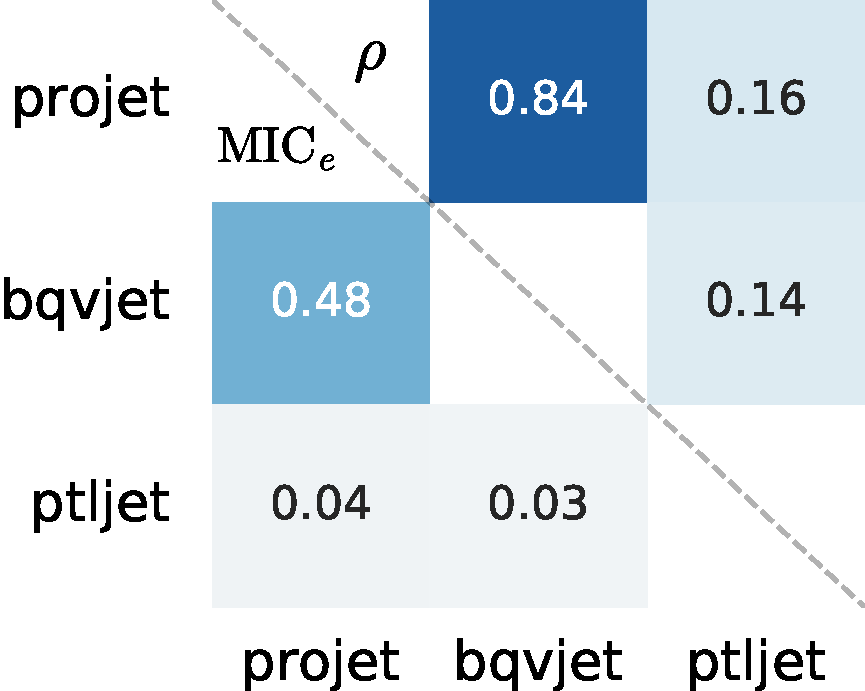
\includegraphics[width=0.31\textwidth]{figures/quarks/correlations_vertex_vars-down_sample=1.00-ML_vars=vertex-selection=b-ejet_min=4-n_iter_RS_lgb=99-n_iter_RS_xgb=9-cdot_cut=0.90-version=19_njet=2.pdf}}}%
  \;
  \subfloat[3-jet events]{{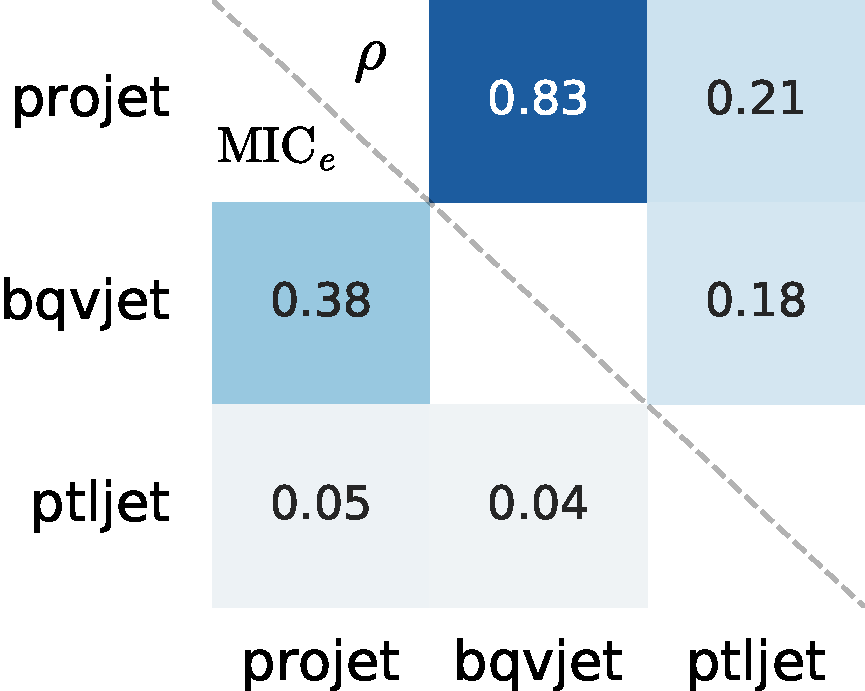
\includegraphics[width=0.31\textwidth]{figures/quarks/correlations_vertex_vars-down_sample=1.00-ML_vars=vertex-selection=b-ejet_min=4-n_iter_RS_lgb=99-n_iter_RS_xgb=9-cdot_cut=0.90-version=19_njet=3.pdf} }}%
  \subfloat[4-jet events]{{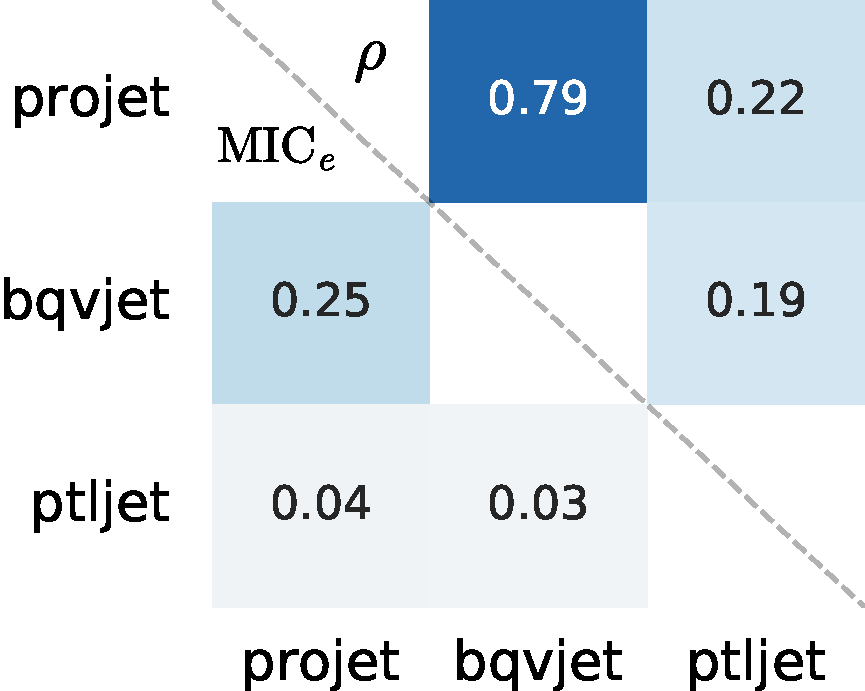
\includegraphics[width=0.31\textwidth]{figures/quarks/correlations_vertex_vars-down_sample=1.00-ML_vars=vertex-selection=b-ejet_min=4-n_iter_RS_lgb=99-n_iter_RS_xgb=9-cdot_cut=0.90-version=19_njet=4.pdf} }}%
  \caption[Correlation of Vertex Variables]{Correlation of the three vertex variables for 2-, 3- and 4-jet events.}%
  \label{fig:q:correlation_vertex_all}%
\end{figure}
\vspace{0.5cm}

% \begin{figure}
%   \centering
%   % \vspace*{-\abovecaptionskip}
%   \subfloat[\label{fig:q:correlation_vertex_2j}]{\;}
%   \subfloat[\label{fig:q:correlation_vertex_2j}]{\;}
%   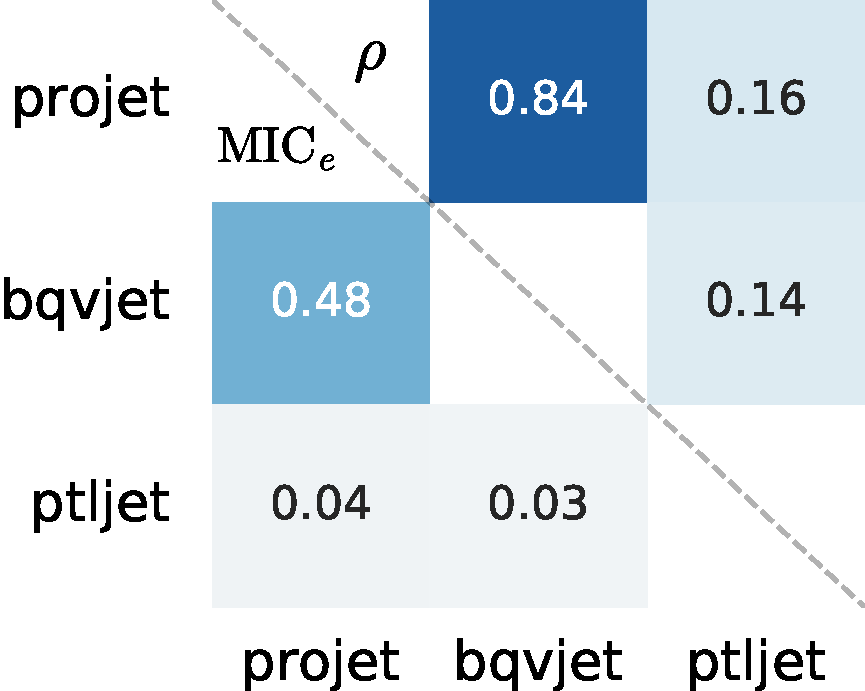
\includegraphics[width=0.28\textwidth]{figures/quarks/correlations_vertex_vars-down_sample=1.00-ML_vars=vertex-selection=b-ejet_min=4-n_iter_RS_lgb=99-n_iter_RS_xgb=9-cdot_cut=0.90-version=19_njet=2.pdf}\hfil
%   \subfloat[\label{fig:q:correlation_vertex_3j}]{\;}
%   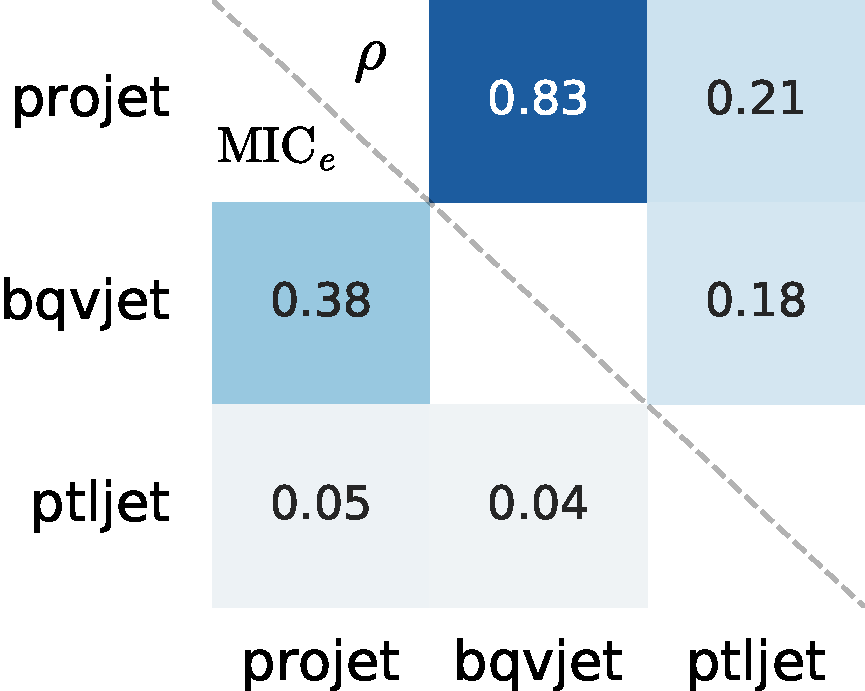
\includegraphics[width=0.28\textwidth]{figures/quarks/correlations_vertex_vars-down_sample=1.00-ML_vars=vertex-selection=b-ejet_min=4-n_iter_RS_lgb=99-n_iter_RS_xgb=9-cdot_cut=0.90-version=19_njet=3.pdf}\hfil
%   \subfloat[\label{fig:q:correlation_vertex_4j}]{\;}
%   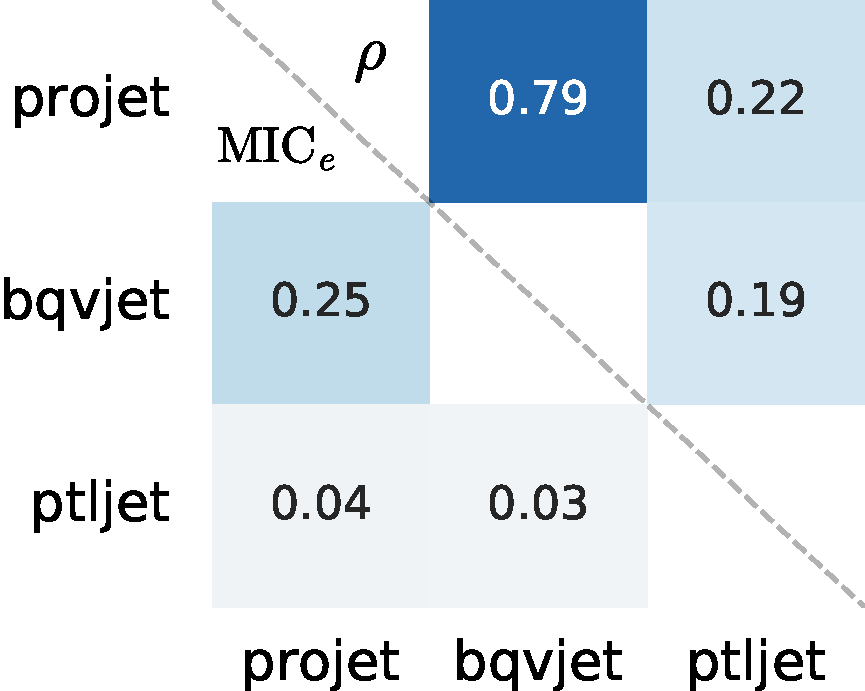
\includegraphics[width=0.28\textwidth]{figures/quarks/correlations_vertex_vars-down_sample=1.00-ML_vars=vertex-selection=b-ejet_min=4-n_iter_RS_lgb=99-n_iter_RS_xgb=9-cdot_cut=0.90-version=19_njet=4.pdf}\hfil
%   \caption[Correlation of Vertex Variables]{Correlation of the three vertex variables for . 
%            Subplot ~\protect\subref{fig:q:correlation_vertex_2j} shows the date of the sale, 
%            Subplot ~\protect\subref{fig:q:correlation_vertex_3j} shows the type of residence,
%            Subplot ~\protect\subref{fig:q:correlation_vertex_4j} shows the area og the house.}
%   \label{fig:q:correlation_vertex_all}
%   \vspace{\abovecaptionskip}
% \end{figure}


\FloatBarrier
\section{Loss and Evaluation Function}
\label{sec:q:loss_evaluation_function}

In contrary to the housing prices subproject the goal in this project is to predict the class of particles, or the types of jets, where the so-called \emph{signal} observations\sidenote{Often called \emph{signal events}, however, this term would require that each event constitutes a single data point in the dataset which it does not here.} are often assigned the label \num{1} and \emph{background} observations \num{0}.  
The combination of this being a \emph{classification} problem (compared to a regression problem) along with the fact all the variables are actual measurements from a particle physics accelerator means that the issue of outliers is negligible. This also means that the problem of finding a robust loss function is non-existent since the in classification loss is already bounded in the $[0, 1]$-interval. 

Classically \emph{accuracy} is often used as loss function for classification which is simply the fraction of correct predictions, however, accuracy as a metric suffers a lot when handling \emph{imbalanced} data: when the ratio between the number of instances of each class is not approximately $(50:50)\si{\percent}$. The problem is that if the sample contains \SI{90}{\percent} background and only \SI{10}{\percent} signal, then a simple model which simply predicts everything to be background will have a \SI{90}{\percent} accuracy.

To circumvent this issue, the area under the ROC curve (AUC) is used, where the ROC\sidenote{Receiver Operating Characteristic.} curve is the the \emph{signal efficiency} $\varepsilon_\mathrm{sig}$ of the ML model plotted as a function of the \emph{background efficiency} $\varepsilon_\mathrm{bkg}$. The definition of these two measures are:
\begin{equation}
  \varepsilon_\mathrm{sig} = \frac{S_\mathrm{sel}}{S_\mathrm{tot}}\,, \qquad \varepsilon_\mathrm{bkg} = \frac{B_\mathrm{sel}}{B_\mathrm{tot}}\,,
\end{equation}
where $S_\mathrm{sel}$ are signal events that were also selected (predicted) as signal by the ML model, $S_\mathrm{tot}=S_\mathrm{sel}+S_\mathrm{rej}$ is the total number of signal events (the selected and rejected), and likewise for background events $B$. Within the machine learning community the signal efficiency is called the true positive rate (TPR) and the background efficiency the false positive rate (FPR). For the rest of this project, the AUC will be the evaluation function $f_\mathrm{eval} = \mathrm{AUC}$, however, since this metric does not work on single observations it cannot be used as the loss function. Instead we will use the \emph{log-loss} as the loss function\sidenote{In the context of machine learning this is the same as the \emph{cross entropy}.} which not not only is differentiable for single predictions, compared to AUC, but also takes the certainty of the prediction into account. When using tree-based algorithms or neural networks one can extract not only whether or not a single observation is classified as signal or background but also a prediction score. This is a number in the $[0, 1]$-interval and the closer to \num{1} the score is, the more certain the model is of the prediction being signal. Given the prediction score $\hat{y}$ and the true label $y$, the log-loss $\ell_\mathrm{log}$ is calculated as:
\begin{equation}
    \ell_\mathrm{log} = -y \log{\hat{y}} - (1-y) \log{(1-\hat{y})}.
\end{equation}
This is visualized in Figure~\ref{fig:q:logloss}. Here it can be seen how the loss changes as a function of the prediction score. Notice that when $y=0$ the loss for $\hat{y}=1$ diverges towards $\infty$ and likewise with $y=1$ and $\hat{y}=0$ (since $\log 0$ diverges to $-\infty$).

\begin{marginfigure}
  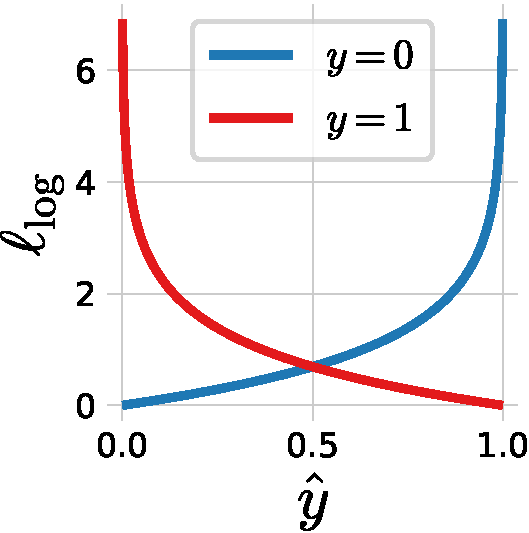
\includegraphics[draft=false, width=0.9\textwidth]{figures/log_loss_cross_entropy/logloss.pdf}
  \caption[Plot of the log-loss $\ell_\mathrm{log}$]
          {Plot of the log-loss $\ell_\mathrm{log}$.} 
  \label{fig:q:logloss}
\end{marginfigure}

\FloatBarrier
\section[b-Tagging Analysis]{$b$-Tagging Analysis}
\label{sec:q:b_tagging_analysis}

The ability to discriminate between the different types of particles produced in a collision is obviously import to understand the results. Today much work go into tagging algorithms from $b$-tagging in ATLAS and CMS \autocite{scodellaroTaggingATLASCMS2017} but this work started even decades ago. That $b$-quarks are tagged specifically is both due to $b$-quarks having more unique characteristics compared to e.g. $c$-quarks and are thus easier to tag, but also the fact that $b$-quarks are the second-heaviest of the quarks and are measured to better understand CP\sidenote{Short for charge-parity.}-violation at LHC-b, contributes to the choice of tagging $b$-quarks. In ALEPH \citet{proriolTAGGINGQUARKEVENTS1991} started the work of comparing different methods for $b$-tagging already in \num{1991}. They concluded that a neural network had the best performance compared to e.g. a linear (Fisher) discriminant. The neural network used was a 3-layer neural network (NN) trained on nine variables and the output \code{nnbjet}. For this of this project this pre-trained network will be called NNB. 

The data are split\sidenote{After removing all low-energy jets such that all events that contain any jets with an energy of less than \SI{4}{\GeV} are removed.} into training and test sets in such a way that the individual jets in an event are not split. As such, the splitting is performed at event-scale in a $(80:20)\si{\percent}$ train-test ratio. 

\begin{margintable}[1cm]
  \centerfloat
  % \vspace{3mm}
  \begin{tabular}{@{}ll@{}}
  Hyperparameter          &  Range                                  \\ \midrule
  \code{subsample}        & $\mathcal{U}(0.4, 1)$                   \\
  \code{colsample_bytree} & $\mathcal{U}_\mathrm{trunc}(0.4, 1, 2)$ \\
  \code{max_depth}        & $\mathcal{U}_\mathrm{int}(-5, 63)$      \\
  \code{num_leaves}       & $\mathcal{U}_\mathrm{int}(7, 4095)$     \\
  \end{tabular}
  % \vspace{\abovecaptionskip}
  \vspace{3mm}
  \caption[Random Search PDFs for LGB]{\label{tab:q:hpo_ranges_lgb}Probability Density Functions for the random search hyperparameter optimization process for the LightGBM model. For an explanation of $\mathcal{U}_\mathrm{trunc}$, see \autoref{sec:q:trunc_uniform}. All negative values of \code{max_depth} are interpreted as no max depth by both LGB and XGB.}
\end{margintable}

\subsection{$b$-Tagging Hyperparameter Optimization}

Compared to the housing prices dataset, the number of observations $N$ is a lot larger, although the dimensionality $M$ is much smaller ($3 \ll 143 $). Therefore both XGBoost (XGB) and LightGBM (LGB) were included as models initially since their performance in the housing dataset was very similar but LightGBM was expected to quite a lot faster on this dataset, which also turned out to be the case. The models were hyperparameter optimized (HPO) using random search (RS) since the Bayesian optimization (BO) did not show any performance gains compared to RS. They were run with $5$-fold cross validation and early stopping with a patience of \num{100}. The PDFs for the random search for the LightGBM model can be seen in Table~\ref{tab:q:hpo_ranges_lgb}, and the ones for XGBoost in Table~\ref{tab:q:hpo_ranges_xgb} in the appendix. The random search has been run with \num{100} iterations for LightGBM and only \num{10} for XGBoost since XGBoost is slow at fitting datasets of this size\sidenote{See page \pageref{page:q:timings_b_tag} for a discussion of the timings.}. The results of the HPO for 3-jet and 4-jet events can be seen in Figure~\ref{fig:q:CV_res_iterations_b_tagging}. For 3-jets it can be seen how most of the iterations share about the same performance within $1\sigma$, however some iterations have a significantly decrease in performance. For 4-jets there are not any iterations which share the same bad performance relative to the others as some of the 3-jets. 

\begin{figure*}%
  \centering
  \subfloat{{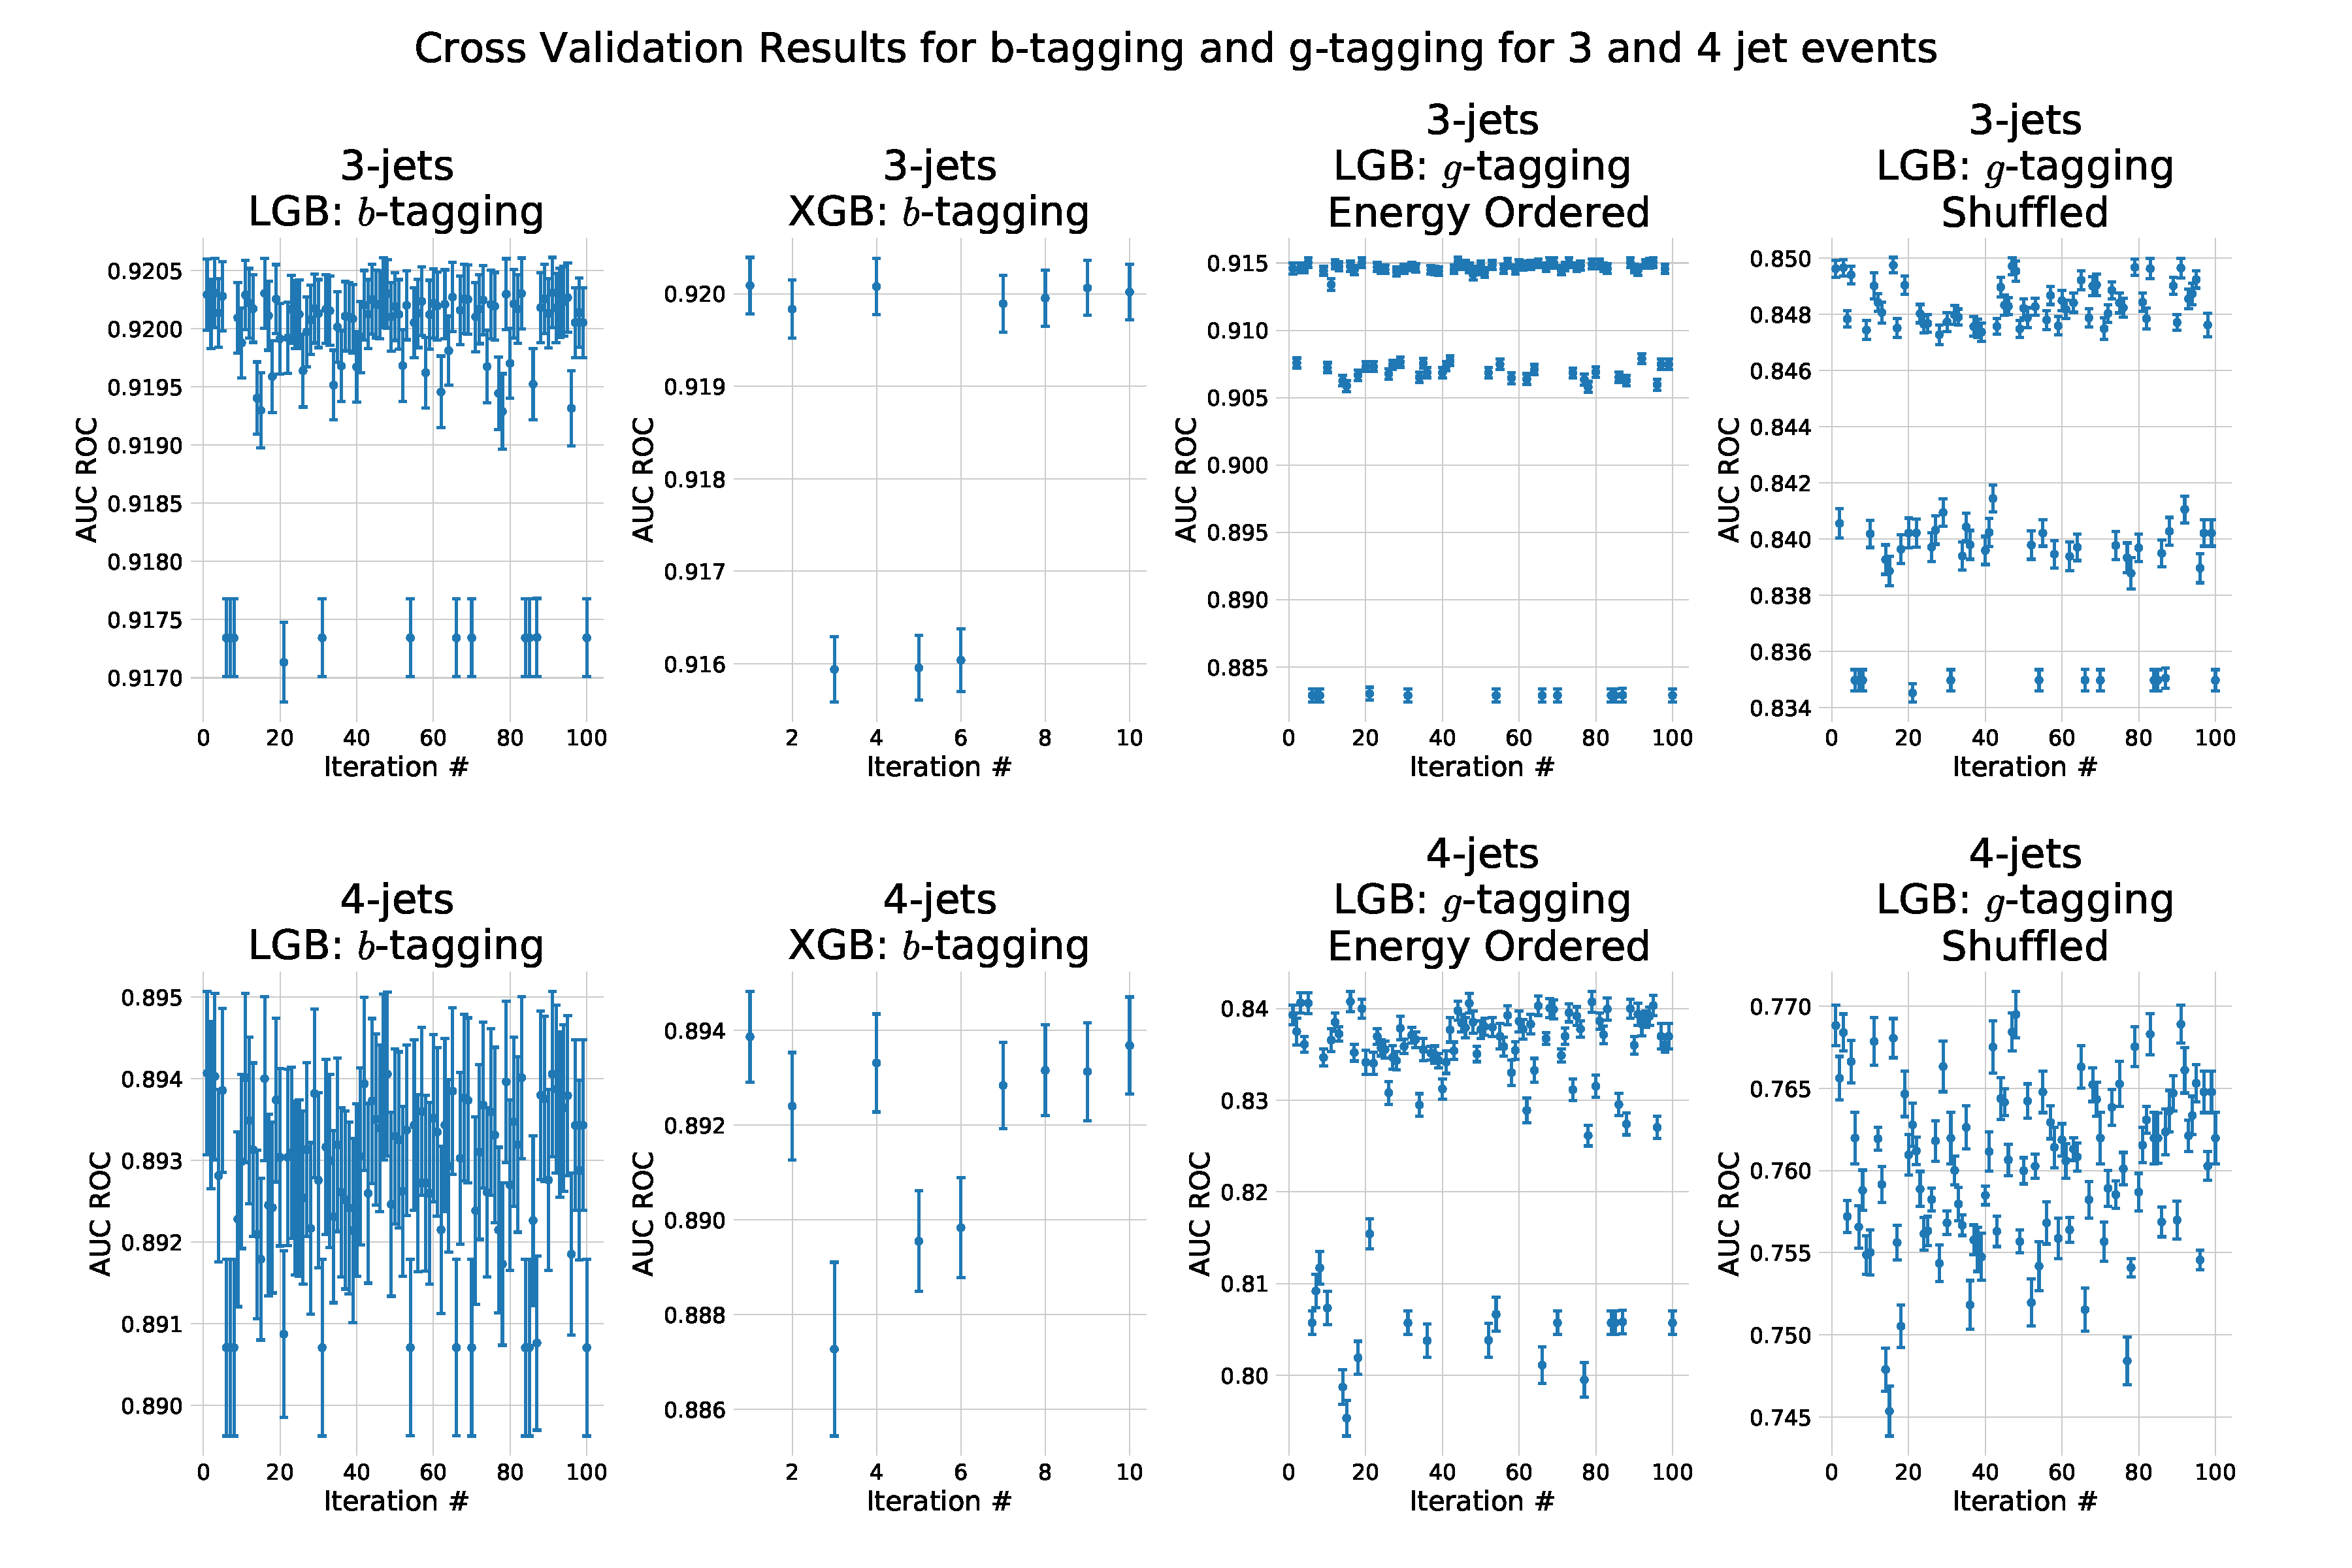
\includegraphics[width=0.48\textwidth, trim=50 580 870 110, clip]{figures/quarks/cv_res_lgb-down_sample=1.00-ML_vars=vertex-selection=b-ejet_min=4-n_iter_RS_lgb=99-n_iter_RS_xgb=9-cdot_cut=0.90-version=19.pdf}}}%
  \;
  \subfloat{{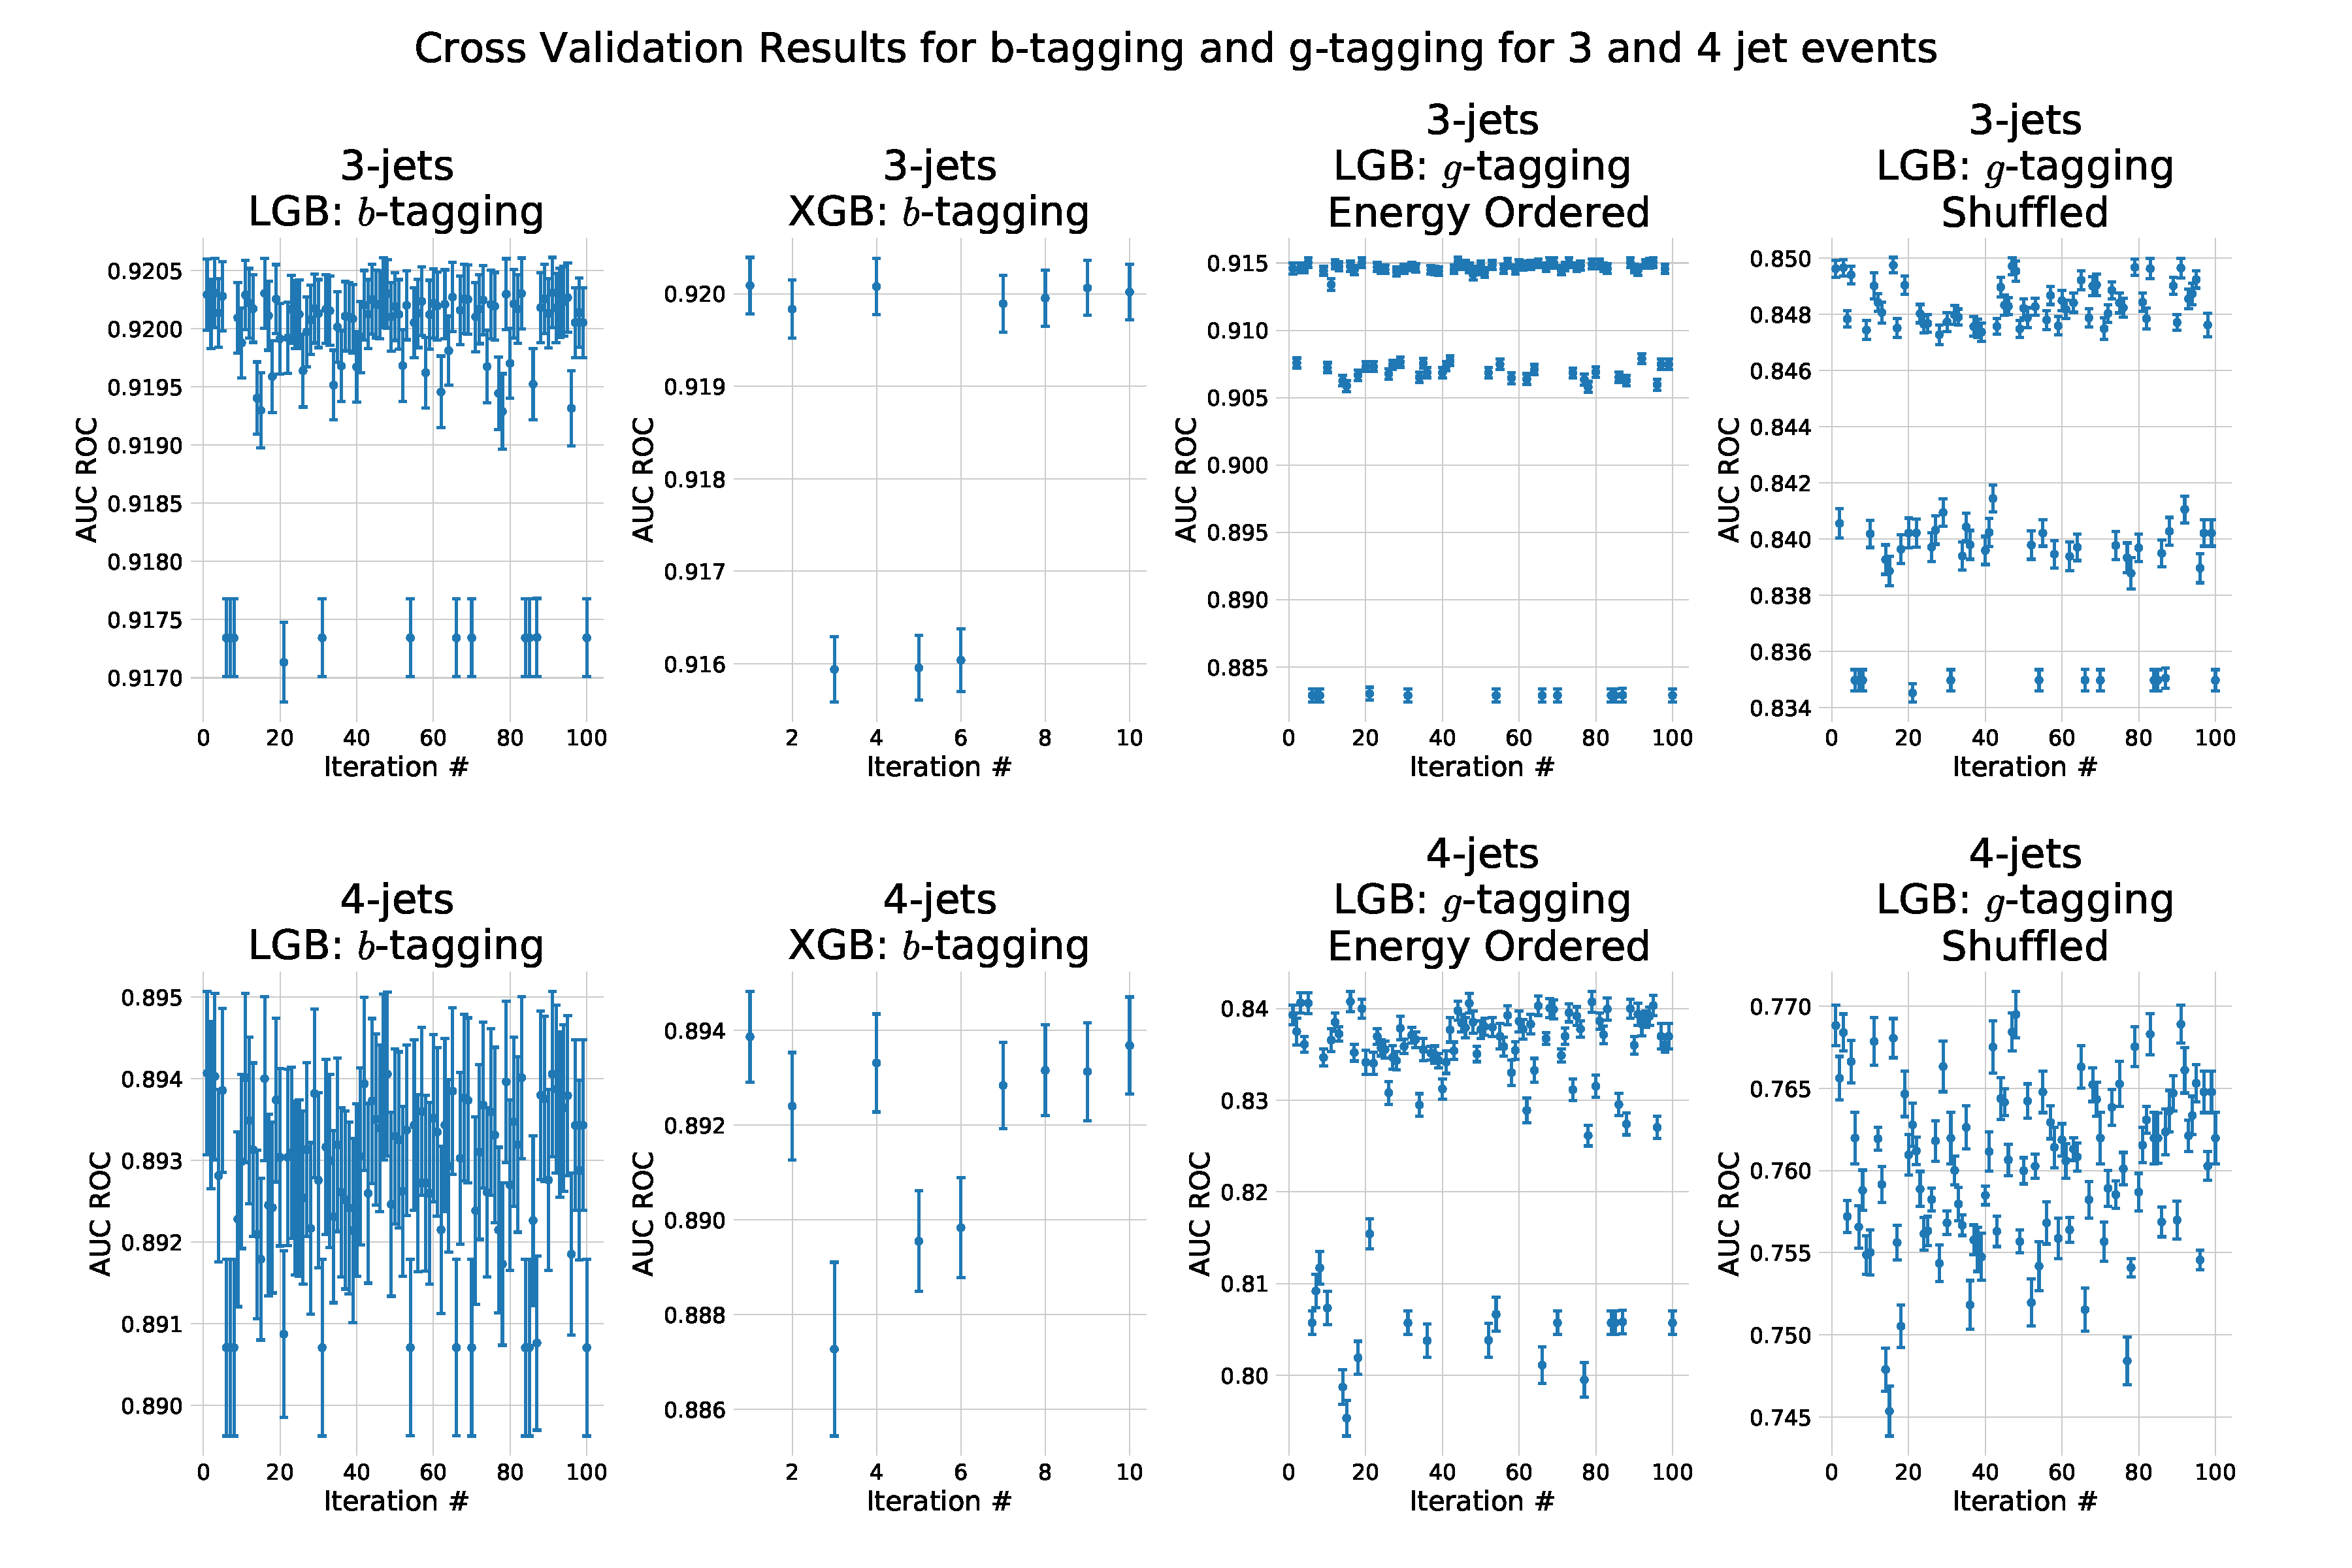
\includegraphics[width=0.48\textwidth, trim=50 40 870 650, clip]{figures/quarks/cv_res_lgb-down_sample=1.00-ML_vars=vertex-selection=b-ejet_min=4-n_iter_RS_lgb=99-n_iter_RS_xgb=9-cdot_cut=0.90-version=19.pdf} }}%
  \vspace{2mm}
  \caption[Hyperparameter Optimization of $b$-tagging]{
    Hyperparameter Optimization results of $b$-tagging with random search. From left to right, we have A) \num{100} iterations of RS with LGB on 3-jets, B) \num{10} iterations of RS with XGB on 3-jets, C) \num{100} iterations of RS with LGB on 4-jets, D) \num{10} iterations of RS with XGB on 4-jets. Notice the different ranges on the y-axes.}
  \label{fig:q:CV_res_iterations_b_tagging}%
\end{figure*}
\vspace{0.5cm}

The relationship between the different hyperparameters in 4-jet events can be seen in the parallel coordinate plot in Figure~\ref{fig:q:initial_CV_res_parallel_coords_4j}. First of all the importance of the column downsampling \code{colsample_bytree} variable is significant: all of the low-performing hyperparameter sets have a low value of this hyperparameter. Since $M=3$ for the vertex variables this makes logical sense; using only $\mathrm{int}(\sim 0.5 \cdot 3) = 1$ variable\sidenote{See \autoref{sec:q:trunc_uniform} for a deeper discussion about the \code{colsample_bytree} hyperparameter.} the model cannot properly learn the structure in the data. Compared to the column downsampling, the other hyperparameters are notably less important. The same overall conclusion can be inferred in the 3-jet case, see Figure~\ref{fig:q:initial_CV_res_parallel_coords_3j} in the appendix.

\begin{figure}
  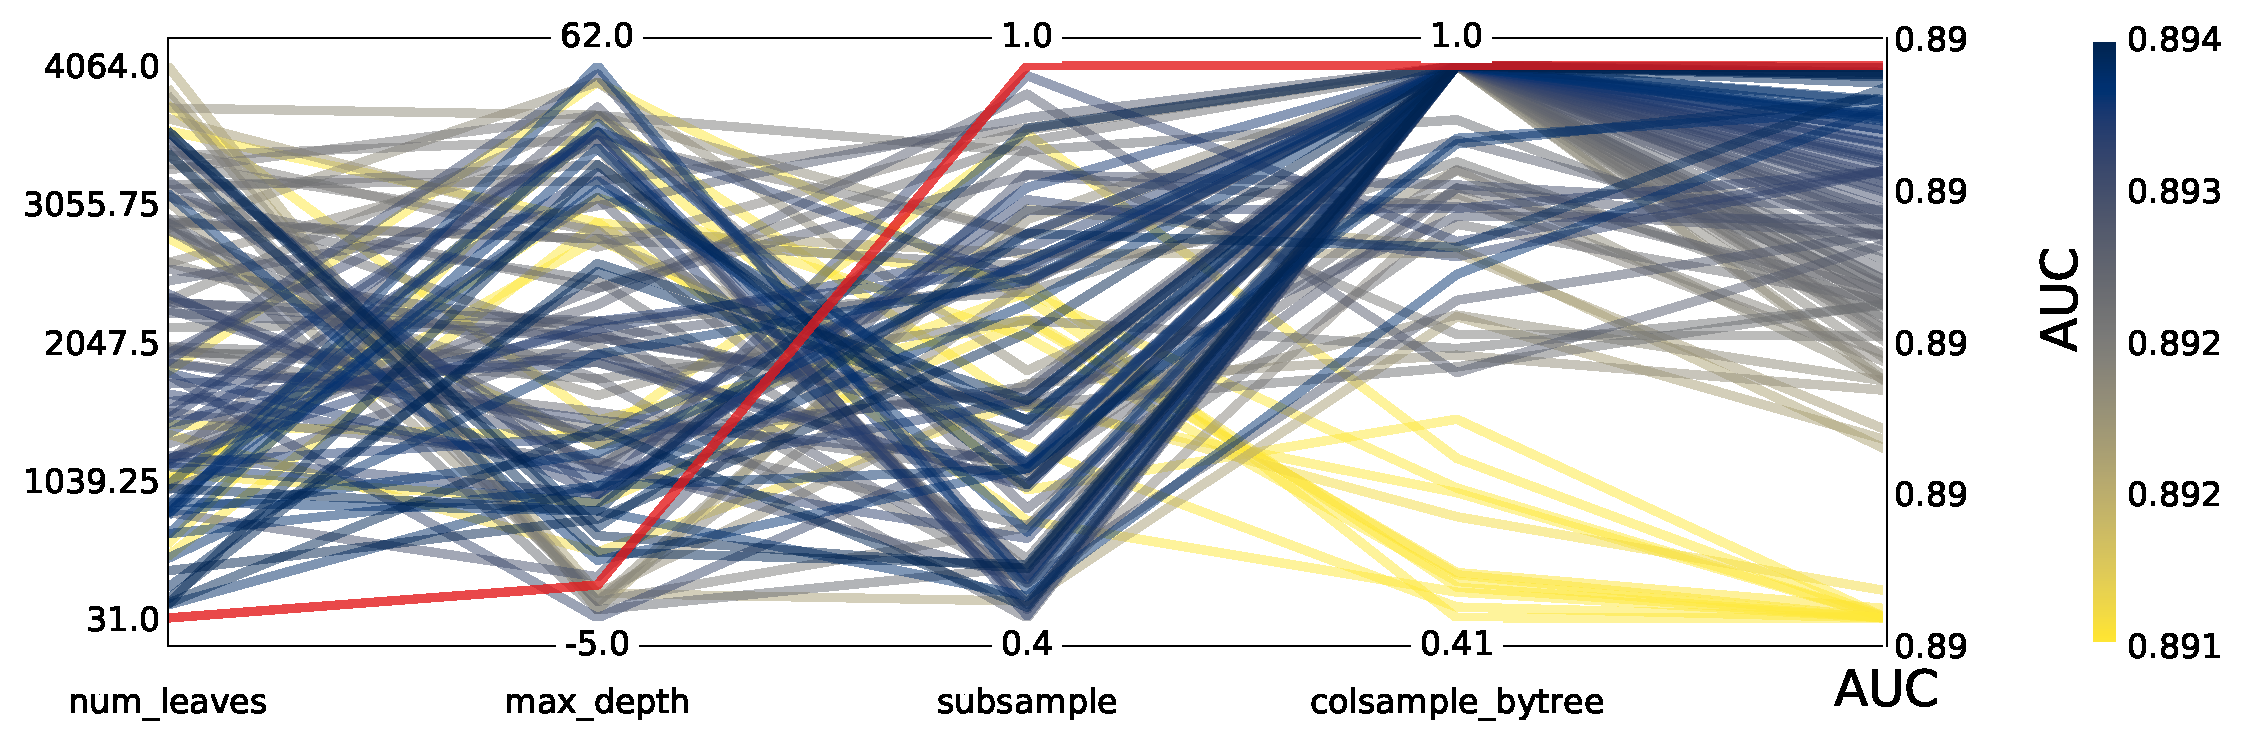
\includegraphics[width=0.98\textwidth, trim=0 0 0 0, clip]{figures/quarks/CV_viz-njet=4-name=lf_lgb_down_sample=1.00-ML_vars=vertex-selection=b-ejet_min=4-n_iter_RS_lgb=99-n_iter_RS_xgb=9-cdot_cut=0.90-version=19.pdf}
  \caption[Parallel Plot of HPO Results for 4-Jet $b$-Tagging]
          {Hyperparameter optimization results of $b$-tagging for 4-jet events. The results are shown as parallel coordinates with each hyperparameter along the $x$-axis and the value of that parameter on the $y$-axis. Each line is an event in the 4-dimensional space colored according to the performance of that hyperparameter as measured by AUC from \textcolor{viridis-dark}{highest} AUC in dark blue to \textcolor{viridis-light}{lowest} AUC in yellow. The \textcolor{red}{single best hyperparameter} is shown in red. 
          } 
  \label{fig:q:initial_CV_res_parallel_coords_4j}
\end{figure}

\subsection{$b$-Tagging Results}

The prediction score for the $b$-tagging models is usually called the $b$-tag and will be written as $\beta_\mathrm{tag}$. The distribution of $\beta_\mathrm{tag}$ for the two HPO-optimized models, LGB and XGB, together with the pre-trained neural network NNB can be seen in Figure~\ref{fig:q:btag_scores_4j} for 4-jet events and in \ref{fig:q:btag_scores_3j} in the appendix for 3-jet events. Notice the strong match between the NNB and LGB models. The XGB model has almost no high $b$-tags $\beta_\mathrm{tag} > 0.8$, but a majority of $b$-tags in the very low end. This indicates that the XGBoost has focussed on the background events compared to the signal events, whereas the NNB and LGB models have focused more on the signal events. 

\begin{figure}[h!]
  \centerfloat
  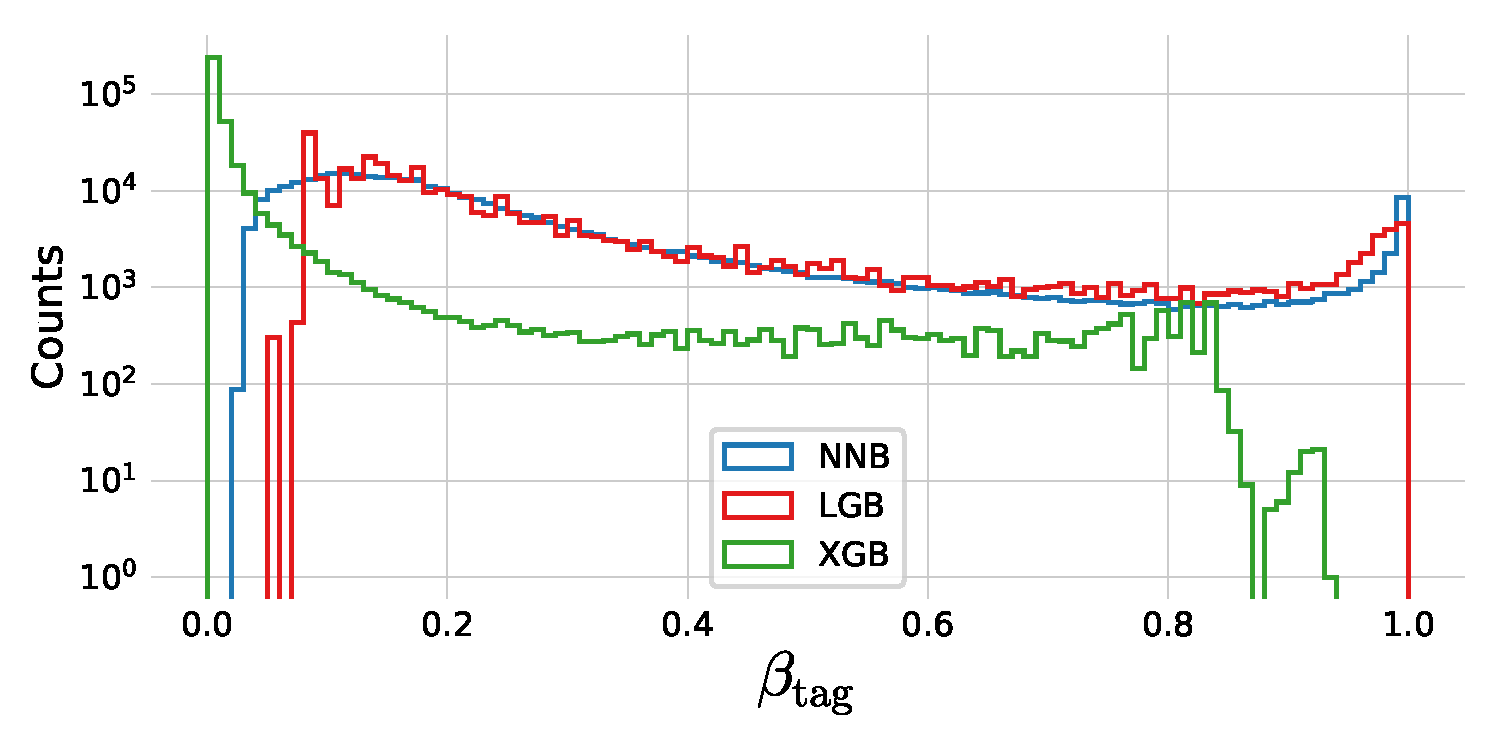
\includegraphics[width=0.95\textwidth, trim=0 0 0 30, clip]{figures/quarks/y_pred_4_jet_hist-down_sample=1.00-ML_vars=vertex-selection=b-ejet_min=4-n_iter_RS_lgb=99-n_iter_RS_xgb=9-cdot_cut=0.90-version=19.pdf}
  \caption[$b$-Tag Scores in 4-Jet Events]
          {Histogram of $b$-tag scores $\beta_\mathrm{tag}$ in 4-jet events for \textcolor{blue}{NNB} (the neural network pre-trained by ALEPH, also called \code{nnbjet}) in blue, \textcolor{red}{LGB} in red, and \textcolor{green}{XGB} in green. 
          } 
  \label{fig:q:btag_scores_4j}
\end{figure}

Even though the distributions of $b$-tags are different between the three models, the real performance plot for classification is the ROC curve seen in Figure~\ref{fig:q:roc_btag_4j} for 4-jet events. Here the signal efficiency $\varepsilon_\mathrm{sig}$ is plotted as a function of the background efficiency $\varepsilon_\mathrm{sig}$ with the AUC shown in the bottom right corner. The LGB and XGB models performs similarly well with an $\mathrm{AUC}=0.896$ compared to the NNB with $\mathrm{AUC}=0.884$. The differences between the models are even smaller for 3-jet events seen in Figure~\ref{fig:q:roc_btag_3j} in the appendix. In general the LGB and XGB models are so similar that they cannot be distinguished from another in any of the plots and their difference in AUC is on the forth decimal point. \label{page:q:timings_b_tag}
However, the LGB model is several times faster than the XGB model. In comparison, \num{10} iterations of HPO using RS on 3-jet events with XGB took more almost \num{34} hours on HEP\sidenote{The local computing cluster.} compared to just \num{23} hours for \num{100} iterations for LGB. The same performance difference was seen in 4-jet events where the timings were \num{4} hours for XGB compared to \num{2.5} hours for LGB, and thus XGB is dropped in all subsequent analysis. 

\begin{figure}[h!]
  \centerfloat
  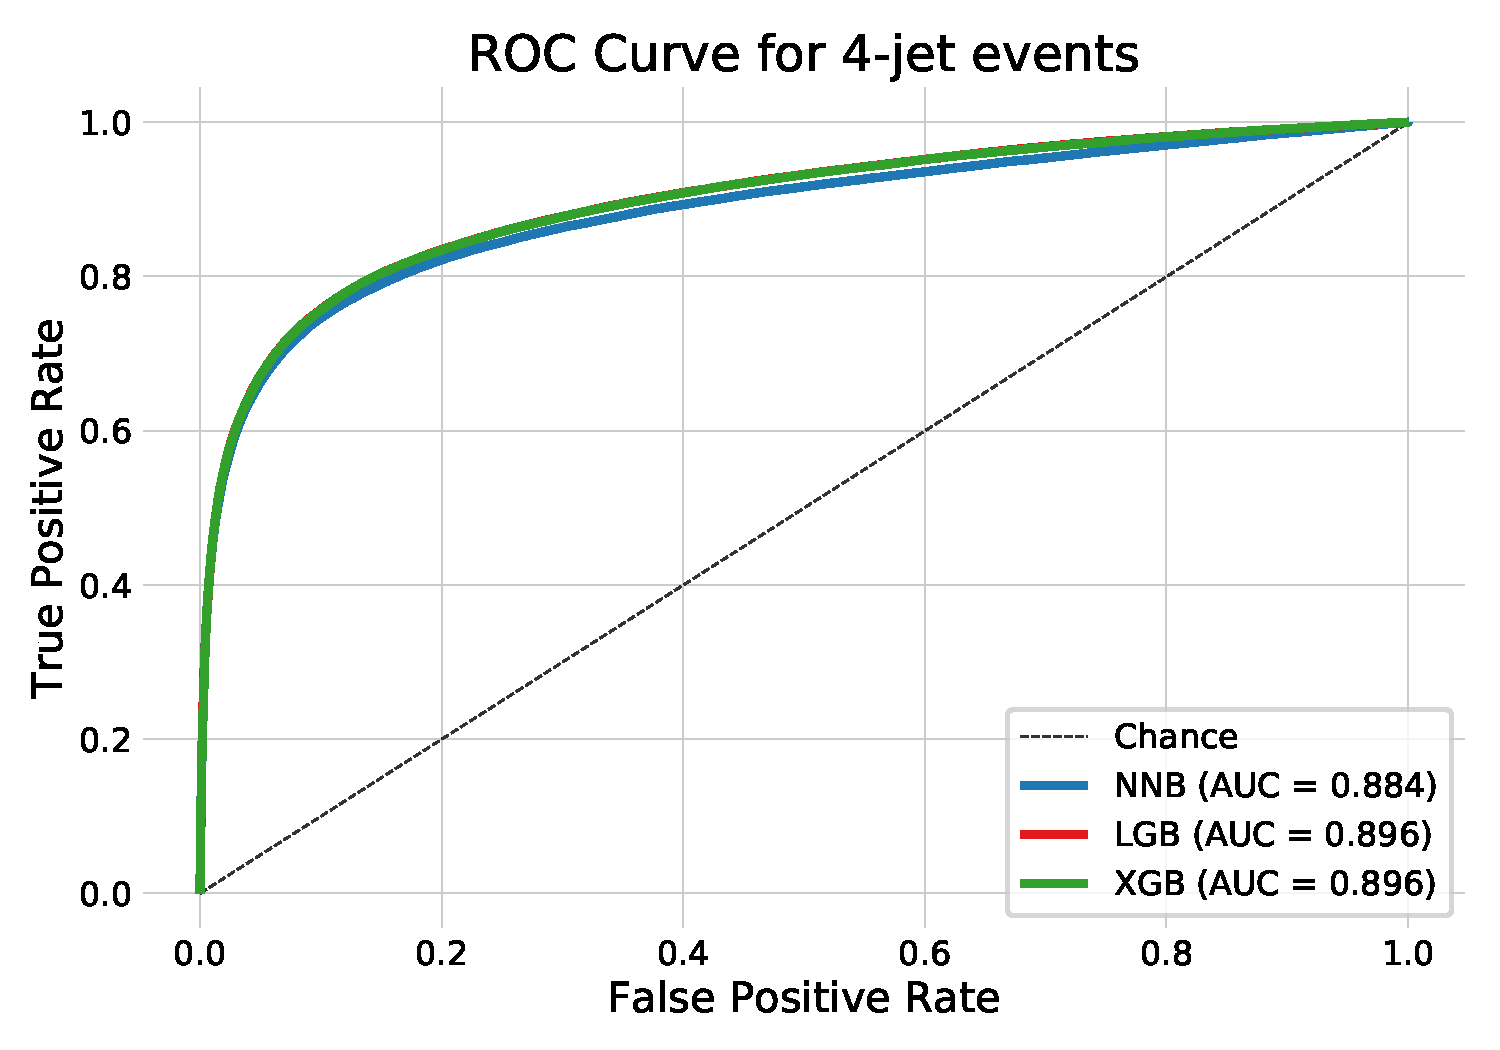
\includegraphics[width=0.95\textwidth, trim=10 10 10 40, clip]{figures/quarks/ROC_4_jet-down_sample=1.00-ML_vars=vertex-selection=b-ejet_min=4-n_iter_RS_lgb=99-n_iter_RS_xgb=9-cdot_cut=0.90-version=19.pdf}
  \caption[ROC curve for 4-jet $b$-tagging]
          {ROC curve of the three $b$-tag models in 4-jet events for \textcolor{blue}{NNB} (the pre-trained neural network trained by ALEPH, also called \code{nnbjet}) in blue, \textcolor{red}{LGB} in red, and \textcolor{green}{XGB} in green. In the legend the area under curve (AUC) is also shown. Notice that the LGB and XGB models share performance and it is thus due to overplotting that only the green line for XGB can be seen. In the machine learning community the background efficiency $\varepsilon_\mathrm{bkg}$ is sometimes know as the false positive rate (FPR) and the signal efficiency $\varepsilon_\mathrm{sig}$ as the true positive rate (TPR).  
          } 
  \label{fig:q:roc_btag_4j}
\end{figure}

\subsection{$b$-Tagging Model Inspection}

To get a better understanding of the trained LGB model, the global SHAP feature importances can be seen in Figure~\ref{fig:q:shap_btag_global_4j} for 4-jet events. First of all it is noted that the \code{projet} has global feature importance of \SI{57.32}{\percent}, \code{bqvjet} \SI{29.16}{\percent}, and \code{ptljet} \SI{13.52}{\percent}. For all three variables it is seen how most of the points have many small feature values which has a negative impact on the model output however small. Especially the \code{ptljet} has many features with a low value (\num{0} in fact) yet this does not pull the model too much towards background events compared to if a jet has a high value of \code{ptljet} which has a strong, positive impact on the output prediction.

\begin{figure}[h!]
  \centerfloat
  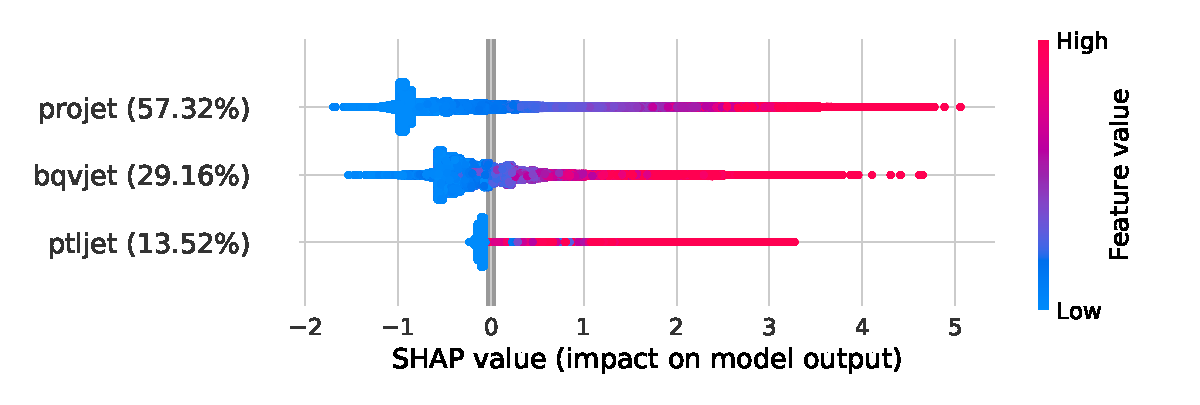
\includegraphics[width=0.98\textwidth, trim=10 10 20 10, clip]{figures/quarks/shap_global-down_sample=1.00-ML_vars=vertex-selection=b-ejet_min=4-n_iter_RS_lgb=99-n_iter_RS_xgb=9-cdot_cut=0.90-version=19-njet=4.pdf}
  \caption[Global Feature Importances for the LGB $b$-Tagging Algorithm on 4-Jet Events]
          {Global feature importances for the LGB $b$-tagging algorithm on 4-jet events. The normalized feature importance is shown in the parenthesis and the each dot is an observation showing the dependance between the SHAP value and the feature's value. 
          } 
  \label{fig:q:shap_btag_global_4j}
\end{figure}

\begin{marginfigure}[-0.5cm]
  \centerfloat
  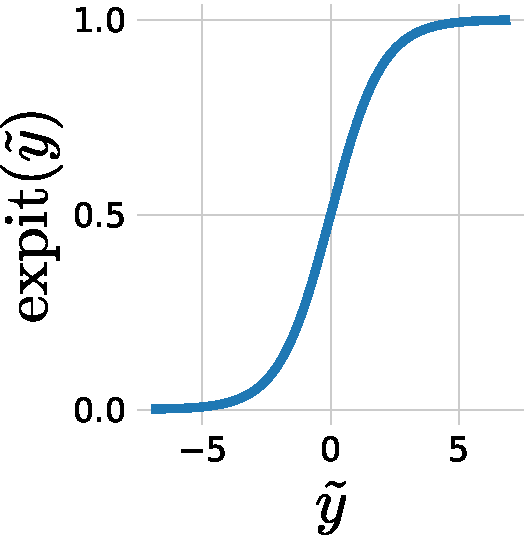
\includegraphics[width=0.8\textwidth]{figures/logit_expit/expit.pdf}
  \caption[The expit Function]
          {The expit function.} 
  \label{fig:q:expit}
\end{marginfigure}

\begin{marginfigure}[0.5cm]
  \centerfloat
  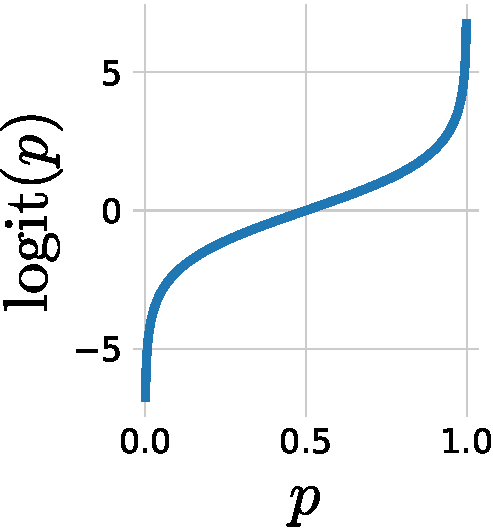
\includegraphics[width=0.8\textwidth]{figures/logit_expit/logit.pdf}
  \caption[The logit Function]
          {The logit function.} 
  \label{fig:q:logit}
\end{marginfigure}

In regression, the model output is a continuous prediction ${\hat{y}_\mathrm{reg} \in \mathbb{R}}$. In classification what is actually happening under the hood is that the model predicts a value $\tilde{y} \in \mathbb{R}$ which is transformed to a number in the $[0, 1]$-interval via the \emph{expit} function:
\begin{equation}
    \label{eq:q:expit}
    \mathrm{expit(\tilde{y})} = \frac{e^{\tilde{y}}}{1+e^{\tilde{y}}} \equiv p,
\end{equation}
where $p$ is a number in the $[0, 1]$-interval. The expit function is also sometimes known as the logistic function and is visualized in Figure~\ref{fig:q:expit}. Its inverse is the \emph{logit} function:
\begin{equation}
  \label{eq:q:logit}
  \mathrm{logit}(p) = \log \left( \frac{p}{1-p}  \right) = \tilde{y},
\end{equation}
 which is visualized in Figure~\ref{fig:q:logit}. The fraction in equation \eqref{eq:q:logit} is called the \emph{odds} and the logit-transformed value of $p$, $\mathrm{logit}(p)=\tilde{y}$, is thus sometimes called the \emph{log-odds}. It is in this log-odds space that LightGBM makes its predictions and the SHAP values in Figure~\ref{fig:q:shap_btag_global_4j} are also in log-odds space. The additivity\sidenote[][0.5cm]{See also \autoref{sec:ml:feature_importance}.} of SHAP is in this log-odds space. 

With this in mind, single predictions of the LGB $b$-tagging model can be understood with SHAP which Figure~\ref{fig:q:shap_single_prediction_3j} is an example of. This figure shows the logic behind the models prediction for this particular jet. That the bias is negative reflects that there is a majority of background compared to signal\sidenote{There are \SI{22.1}{\percent} $b$-jets in the 3-jet training set.}. This particular event has \code{projet}$=1.003$, \code{bqvjet}$=0.529$, and \code{ptljet}$=0$. In the plot it is seen how this high value of \code{projet} has the greatest impact on the model prediction, while the medium value of \code{bqvjet} also pushes the model prediction towards a signal-prediction. The four bars in the left part of the plot are all in log-odds space and their sum is shown as the blue bar to right, where the right $y$-axis shows the value in probability space $p\in [0,1]$. This jet was in fact a $b$-jet.
% , so the model predicted this one correctly. 

\begin{figure}[h!]
  \centerfloat
  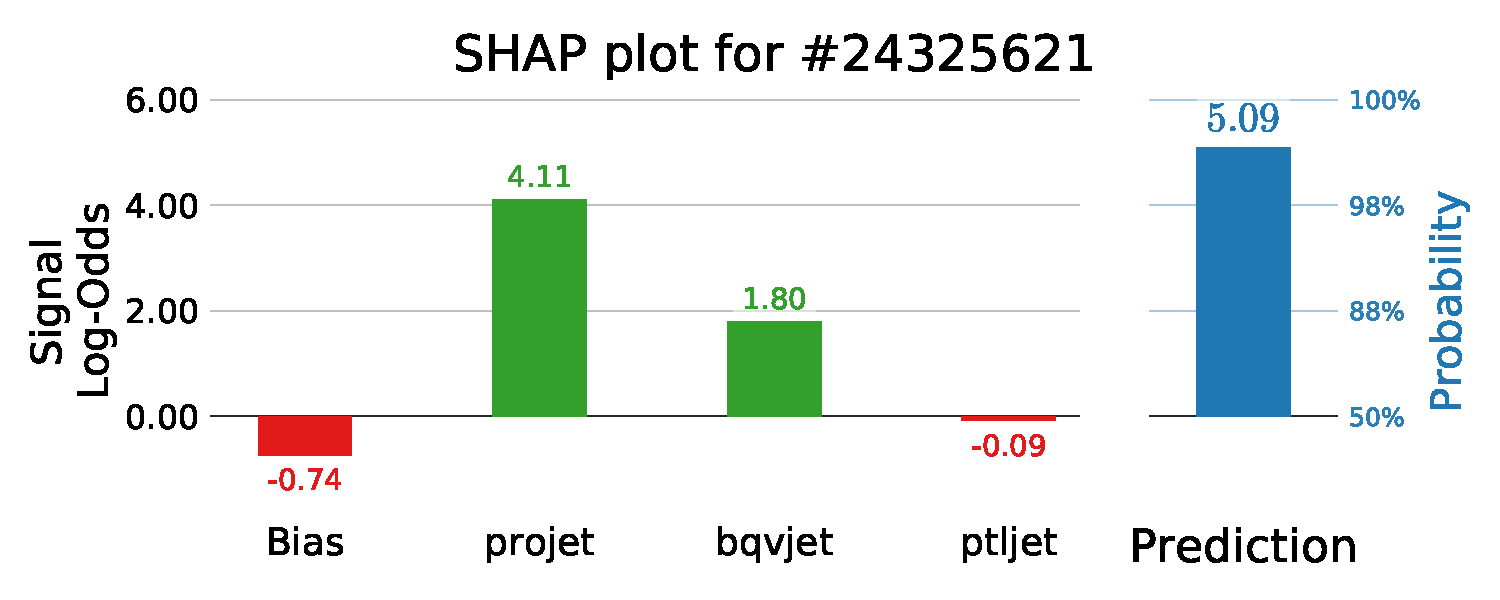
\includegraphics[width=0.95\textwidth, trim=0 0 0 40, clip]{figures/quarks/shap_values-down_sample=1.00-ML_vars=vertex-selection=b-ejet_min=4-n_iter_RS_lgb=99-n_iter_RS_xgb=9-cdot_cut=0.90-version=19-njet=3loc=24325621.pdf}
  \caption[SHAP 3-Jet Model Explanation for $b$-like Jet]
          {Model explanation for the 3-jet $b$-tagging LGB model for a $b$-like jet. The first column is the bias of the training set which acts as the naive prediction baseline, the rest are the input data variables. On the right hand side of the plot is the model prediction shown. The left part of the plot is shown in log-odds space, the right part in probability space. The \textcolor{red}{negative} log-odd values are shown in red, \textcolor{green}{positive} ones in green, and the \textcolor{blue}{prediction} value in blue. 
          } 
  \label{fig:q:shap_single_prediction_3j}
\end{figure}



\section{Truncated Uniform PDF}
\label{sec:q:trunc_uniform}

Initially when plotting the HPO performance as a function of iteration, it was seen how there were three significant plateaus, where the highest plateau (i.e. highest AUC value and thus best score) was only seen in the very first iteration. It was quickly realized that this was due to the very first iteration was being run with the default values of the LGB and XGB models in the custom implementation by the author. However, what was not understood was why this value was performing so much better than random sets of hyperparameters\sidenote{LightGBM and XGBoost of course have chosen their default parameters smartly, however, it one would not expect them to outperform other sets of hyperparameters that clearly.}. During the debugging process the column downsampling \code{colsample_bytree} was diagnosed to be the culprit. The default value is \code{colsample_bytree}$=1$, however, the probability density function (PDF) used in RS for this parameter was $\mathcal{U}(0.4, 1)$ which was expected to give the same performance as the default value for large values of \code{colsample_bytree}. By inspecting the source code of LightGBM it was realized that the model takes the integer of the column downsampling multiplied with the total number of features if the column downsampling is less than \num{1} \autocite{MicrosoftLightGBM}. This means that no matter how close to \num{1} the column downsampling get, the integer value of the total number of columns get floored to \num{2} at max, compared to when the column downsampling is exactly \num{1} which it only is for the default values.

To deal with this problem a new PDF was developed on top of the existing ones in Scipy, the truncated uniform PDF: $\mathcal{U}_\mathrm{trunc}(a, b, c)$. This PDF first generates a random number $x$ from a uniform distribution between $a$ and $c$. Then if $x$ is larger than $b$ it is floored to $b$. In this way, it is possible to both get values of $x$ in the interval $[a, b]$ but also values exactly equal to $b$. The value of $c$ controls how often these \q{overflow} values of $x$ are generated.




\FloatBarrier
\section[g-Tagging Analysis]{$g$-Tagging Analysis}
\label{sec:q:g_tagging_analysis}

The trained $b$-tagging LGB model is a jet-based model which provides a $b$-tag score $\beta_\mathrm{tag}$ to a jet. This also means that each of the jets e.g. a 4-jet event can get a $b$-tag: $\bm{\beta}_\mathrm{tag}=[\beta_{\mathrm{tag}_1}, \beta_{\mathrm{tag}_2}, \beta_{\mathrm{tag}_3}, \beta_{\mathrm{tag}_4}]$. Using $\bm{\beta}_\mathrm{tag}$ one can train a new model on the events, compared to individual jets, where signal events are defined to be $q$-matched events where the gluons are assigned the $n-2$ lowest $b$-tag scores for $n$-jet events; e.g. $\bm{\beta}_\mathrm{tag}=[0.95, 0.89, 0.15, 0.07]^\top$ for the four jets $[b, \bar{b}, g, g]$. This event-based process will be called $g$-tagging and the trained model will return a $g$-tag score written as $\gamma_\mathrm{tag}$. Compared to the $b$-tagging LGB model, this model will allow one to extract entire events which contains a clear identification of gluons versus non-gluons.

\subsection{Permutation Invariance}
\label{subsec:q:permutation_invariance}

Since the $b$-tags are only based on the vertex variables, the goal of the $g$-tag is to also be constructed in an un-biased way with respect to the jet energy $E_\mathrm{jet}$. However, even though $\beta_\mathrm{tag} \Independent E_\mathrm{jet}$ and $\gamma_\mathrm{tag} = f(\beta_\mathrm{tag})$, it turned out that $\gamma_\mathrm{tag} \NotIndependent E_\mathrm{jet}$, where $a \Independent b$ is defined to mean that $a$ is independent\sidenote{And $\NotIndependent$ means not independent.} of $b$ and $f$ is an unknown function. This was because the ordering of the jets within the event was energy-dependent: they sorted according to their $E_\mathrm{jet}$. 

This meant that the different components in $\bm{\beta}_\mathrm{tag}$ had different importances, even though they should be equally important. Instead of defining $\bm{\beta}_\mathrm{tag}$ as a vector it should instead be seen as a set\sidenote{Since sets have no inherent order.} $\bm{\beta}_\mathrm{tag}=\{\beta_{\mathrm{tag}_1}, \dots, \beta_{\mathrm{tag}_n}\}$. The $g$-tagging model trained on the events should thus be \emph{permutation invariant}\sidenote{$f(\vec{x}) = f(\tau(\vec{x}))$ for any permutation $\tau$ on an input vector $\vec{x}$.} with regards to the input variables. The category of permutation invariant (and equivariant\sidenote{$\tau(f(\vec{x})) = f(\tau(\vec{x}))$ for any permutation $\tau$ on an input vector $\vec{x}$.}) neural networks in the deep learning community has seen an huge development within recent years where the paper from \citet{zaheerDeepSets2017} in 2017 was quite influential, however also other examples exists \autocite{ravanbakhshDeepLearningSets2017, guttenbergPermutationequivariantNeuralNetworks2016}. Yet, the same development cannot be said to have happened within the more classic machine learning field.

Although not being a novel software-technical solution, the problem was circumvented by two simple, different approaches: 1) by simply shuffling the inputs variables independently for each observation (row) in the dataset, and 2) training on all possible permutations of the variables in the dataset. The second approach can be seen as a feature augmentation technique where the data is artificially increased with factor of $n$ factorial: $N \rightarrow n!\cdot N$ where $N$ is the number of observations (rows) and $n$ is the number of jets. These two methods were tested along with the original order of the dataset. 

\subsection{$g$-Tagging Hyperparameter Optimization}

Four LightGBM models, two for 3-jet events and two for 4-jet events, were trained and hyperparameter optimized for both the the energy ordered and shuffled\sidenote[][2cm]{The method with all permutations was trained using the same hyperparameters as the best ones for the shuffled model.} data sets with \num{100} iterations of random search with the same PDFs as for the $b$-tagging, see Table~\ref{tab:q:hpo_ranges_lgb}, and $5$-fold cross validation and early stopping with a patience of \num{100}. The results of the HPO can be seen in Figure~\ref{fig:q:CV_res_iterations_g_tagging}. Here the two 3-jets models are seen in the two plots to the left, and the two 4-jets to the right. The very left plot shows the 3-jet energy-ordered (no permutation) performance as a function of iteration number, which was also where the issues mentioned in \autoref{sec:q:trunc_uniform} were first discovered. Here the difference between the how many of the three variables, the three $b$-tags, are included is seen as three clear plateaus. The three plateaus are also seen in the 3-jet events that were shuffled, however, with more variation in each plateau, along with a drop in performance. For the 4-jet events the plateaus are not as apparent but it can still be seen how some of the iterations how a significantly lower score than others. The parallel plots for the four fits can be seen in Figure~\ref{fig:q:CV_res_parallel_coords_g_tag_3j_energy_ordered}--\ref{fig:q:CV_res_parallel_coords_g_tag_4j_shuffled} in the appendix.

\begin{figure*}%
  \centering
  \subfloat{{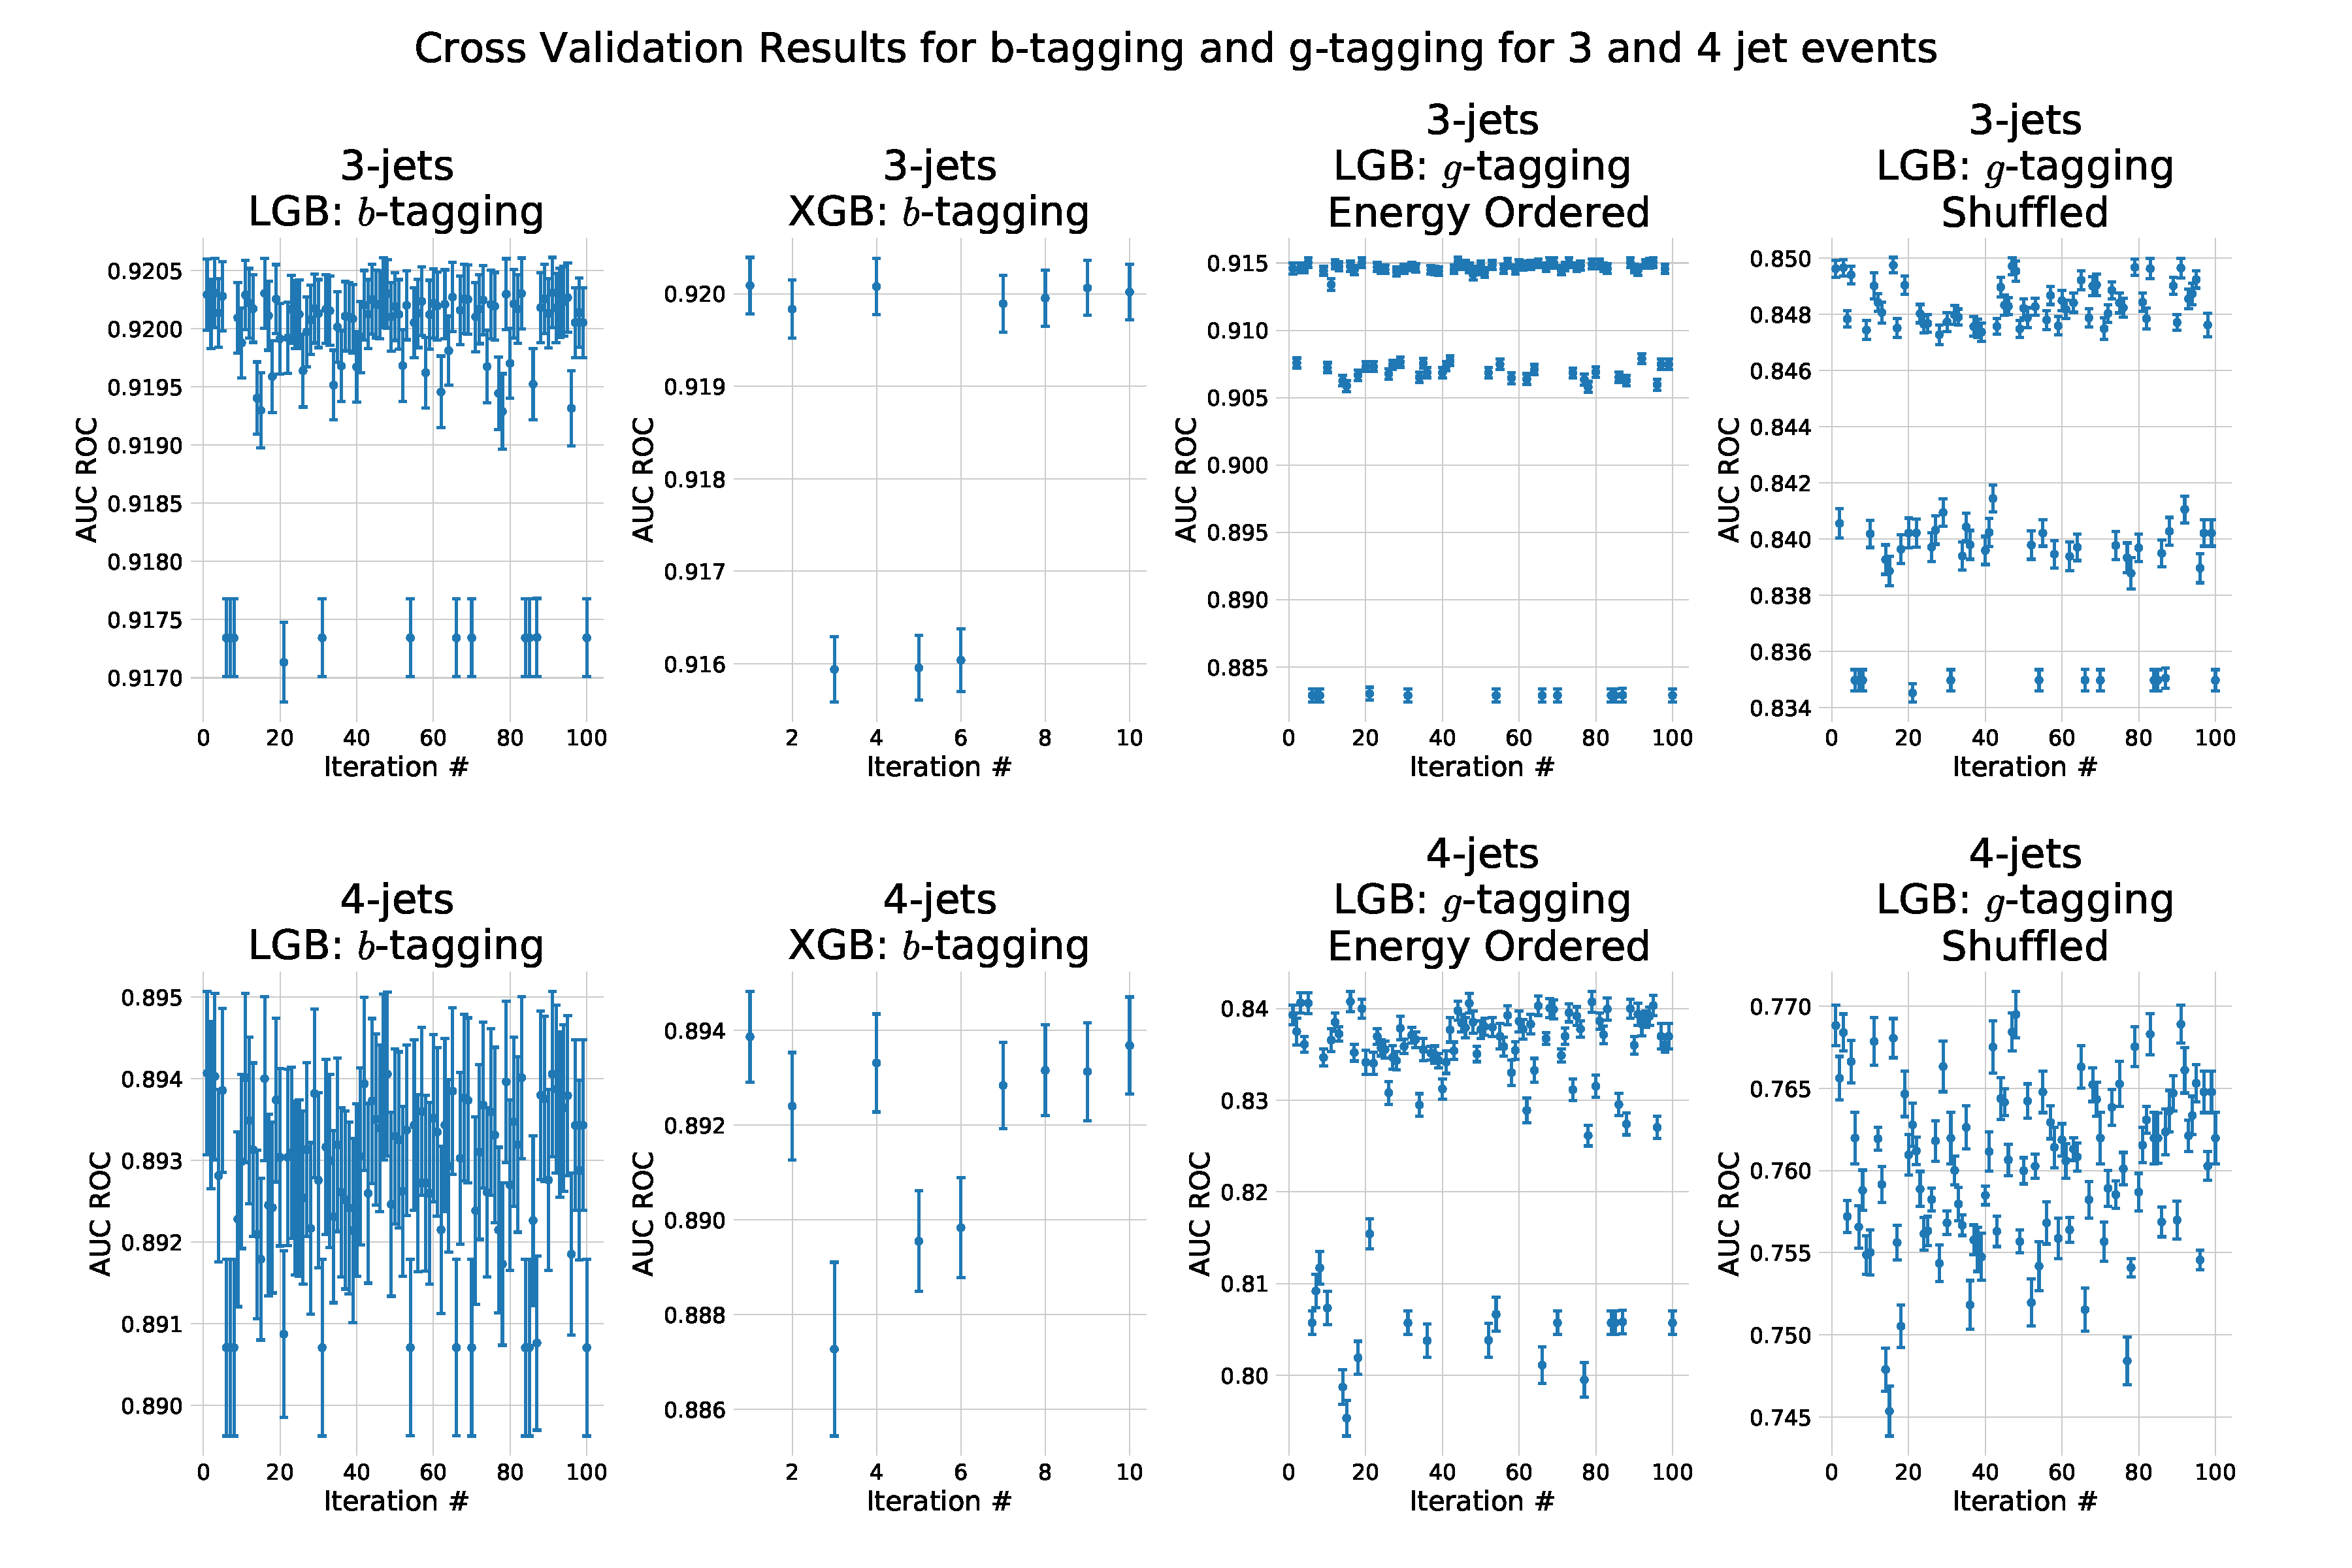
\includegraphics[draft=false, width=0.48\textwidth, trim=860 580 50 70, clip]{figures/quarks/cv_res_lgb-down_sample=1.00-ML_vars=vertex-selection=b-ejet_min=4-n_iter_RS_lgb=99-n_iter_RS_xgb=9-cdot_cut=0.90-version=19.pdf}}}%
  \;
  \subfloat{{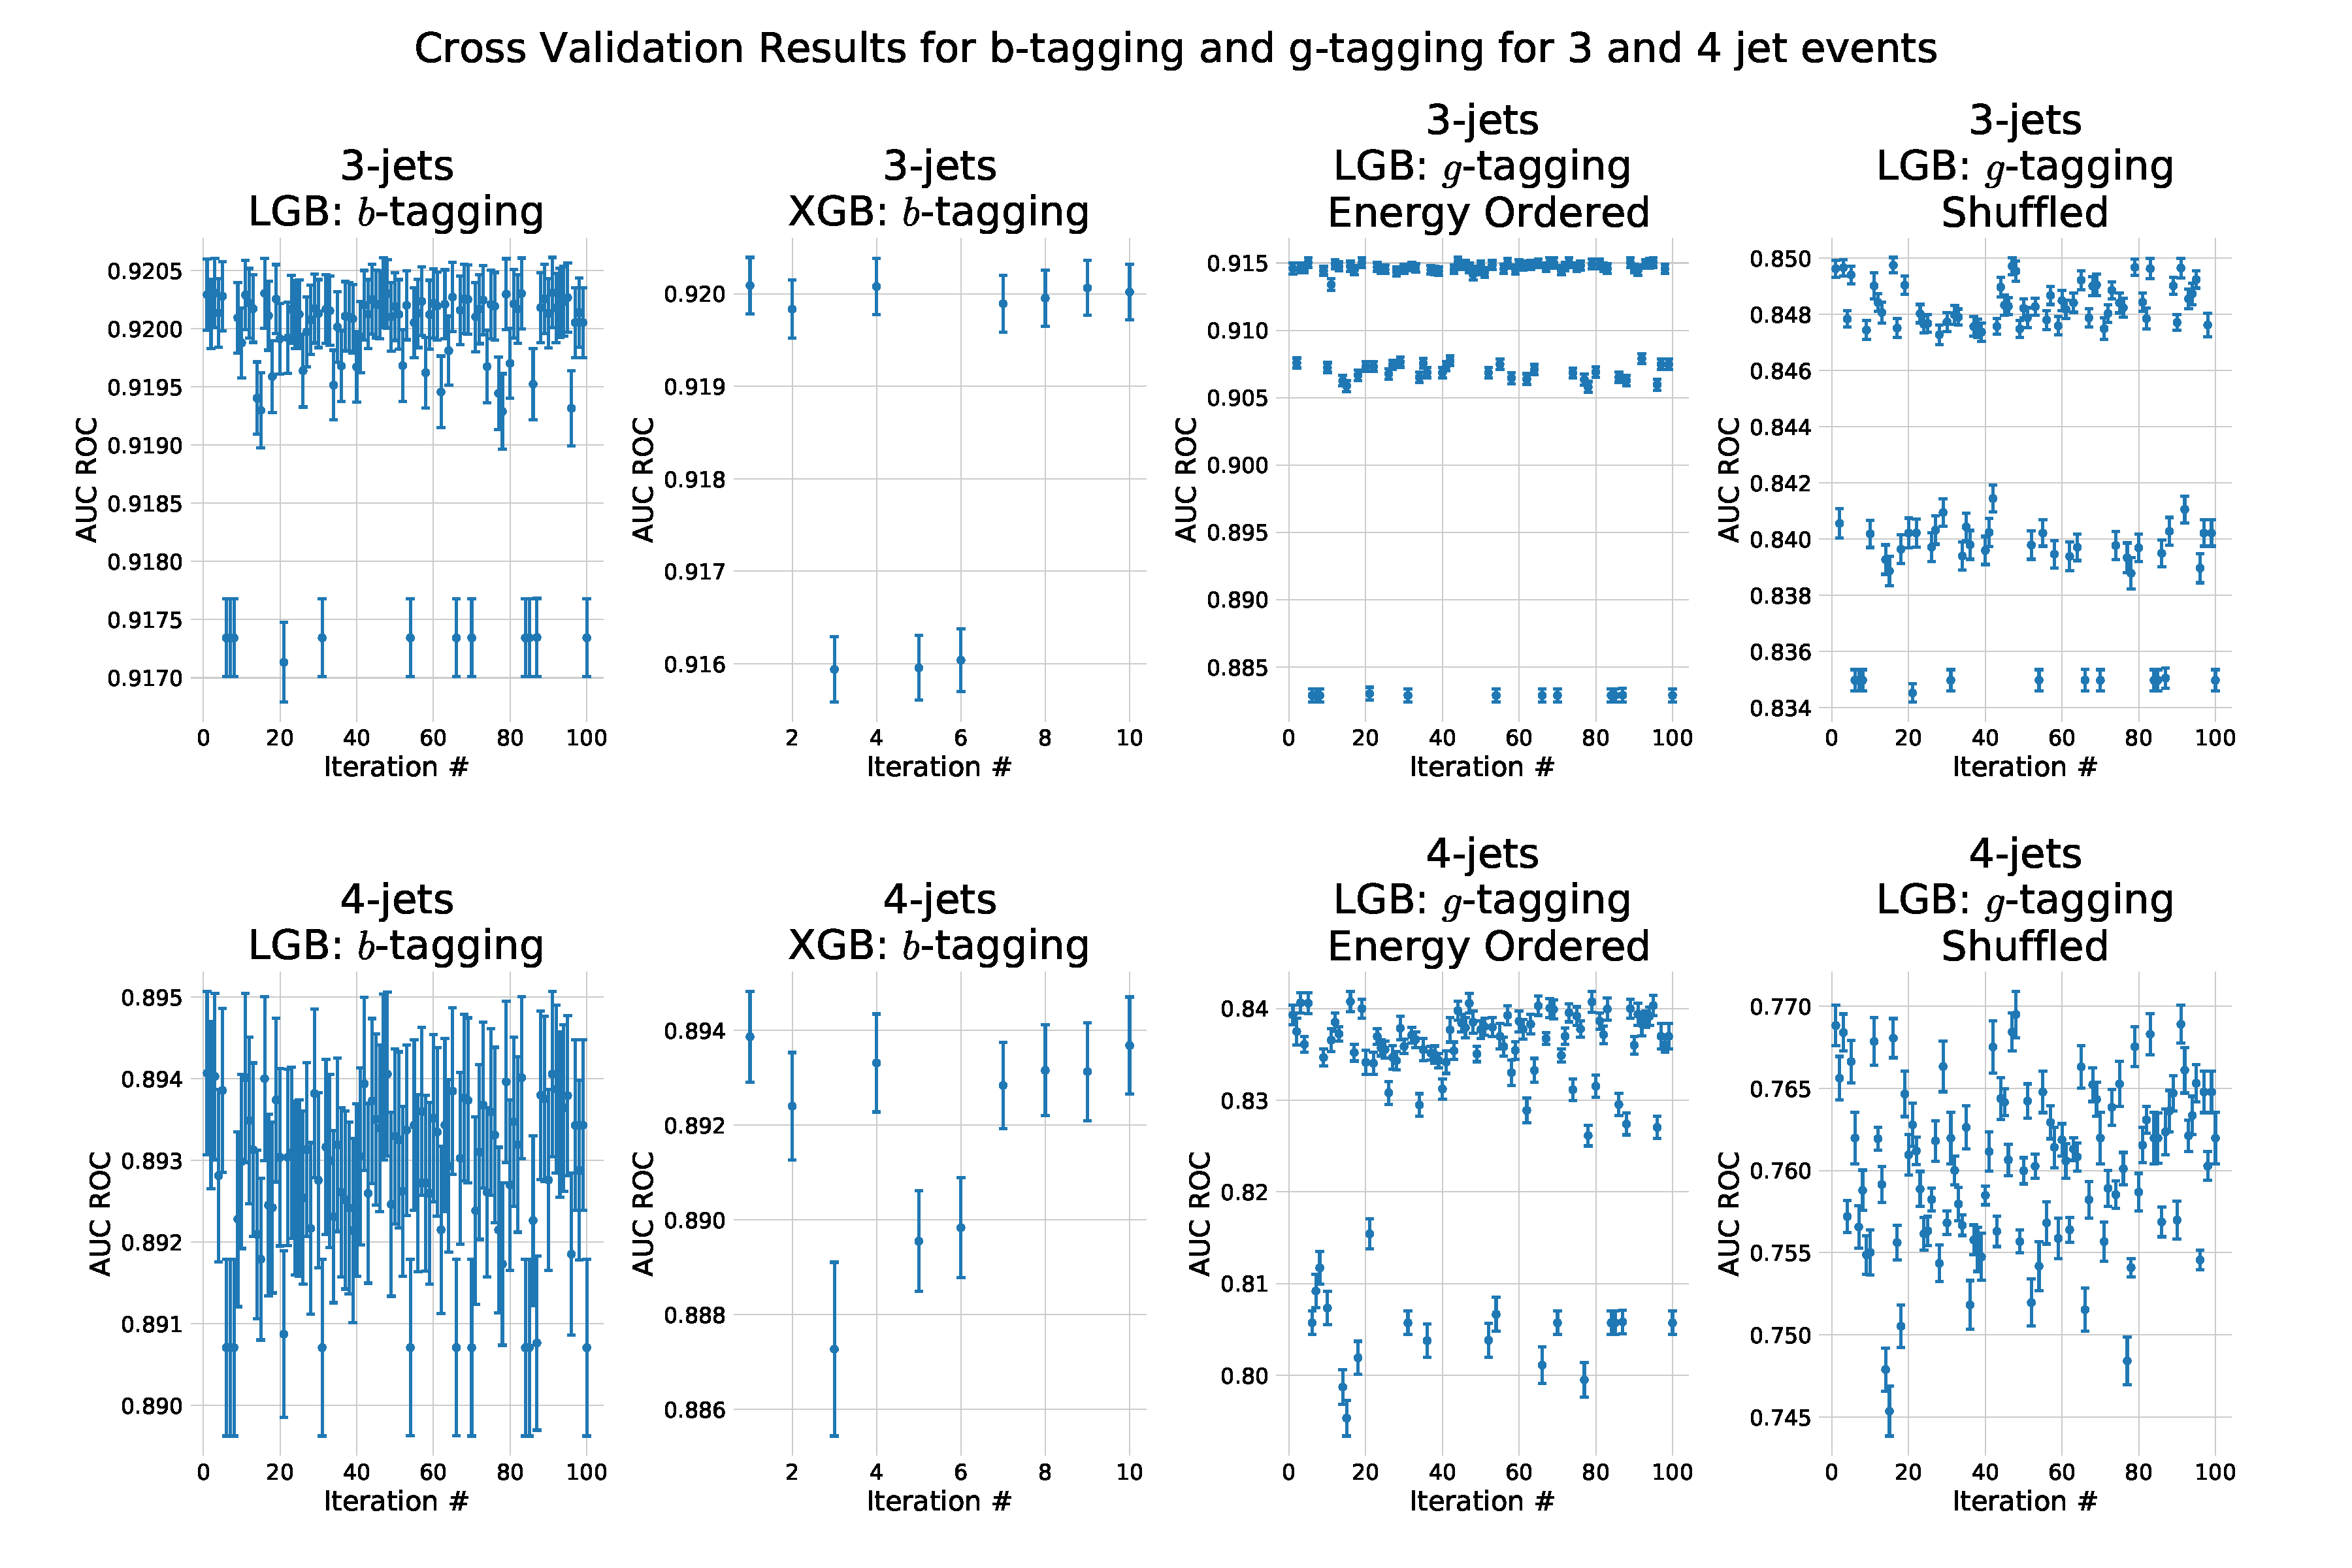
\includegraphics[draft=false, width=0.48\textwidth, trim=870 40 40 610, clip]{figures/quarks/cv_res_lgb-down_sample=1.00-ML_vars=vertex-selection=b-ejet_min=4-n_iter_RS_lgb=99-n_iter_RS_xgb=9-cdot_cut=0.90-version=19.pdf} }}%
  \vspace{2mm}
  \caption[Hyperparameter Optimization of $g$-tagging]{
    Hyperparameter Optimization results of $g$-tagging with \num{100} iterations of random search with LGB. From left to right, we have A) 3-jet events energy-ordered (no permutations), B) 3-jet events row-shuffled, C) 4-jet events energy-ordered, D) 4-jet events row-shuffled. Notice the different ranges on the y-axes.}
  \label{fig:q:CV_res_iterations_g_tagging}%
\end{figure*}

\subsection{PermNet}
\label{subsec:q:permnet}

In addition to the LGB models, a permutation invariant neural network called PermNet based on the Deep Sets paper \autocite{zaheerDeepSets2017} implemented in Tensorflow \citep{tensorflow2015-whitepaper} by \citet{fayeFrederikFayeDeepcalo} was also tested. \citet{zaheerDeepSets2017} showed that $f(X)$ is permutation invariant if and only if it can be decomposed in the following way:
\begin{equation}
  \label{eq:q:deep_sets}
  f(X)=\rho\left(\sum_{x\in X} \phi(x) \right).
\end{equation}
for suitable transformations $\rho$ and $\phi$ (which the neural network learns\sidenote{This is possible since neural networks are universal function approximators \autocite{hornikApproximationCapabilitiesMultilayer1991}.}). The PermNet was trained using three layers\sidenote{Where the two hidden layers have \num{128} and \num{64} neurons in each.} with leaky ReLU \autocite{Maas2013RectifierNI} as the activation function and ADAM \autocite{kingmaAdamMethodStochastic2014} as the optimizer optimizing the log-loss. The network was trained with early stopping with a patience of \num{50} epochs and a batch size of \num{128}. A visual overview of the PermNet architecture can be seen in Figure~\ref{fig:q:permnet_architecture} in the appendix.

\subsection{1D Comparison of LGB and PermNet}
\label{subsec:q:lgb_permnet_comparison}

To better understand the difference between the difference between the LGB and PermNet models, a small comparison was made. This comparison was constructed by summing the $b$-tag scores in the $n$-jet event together $\sum_i^n \beta_{\mathrm{tag}_i}$.














\newpage

\vspace{0.5cm}







\begin{figure}
  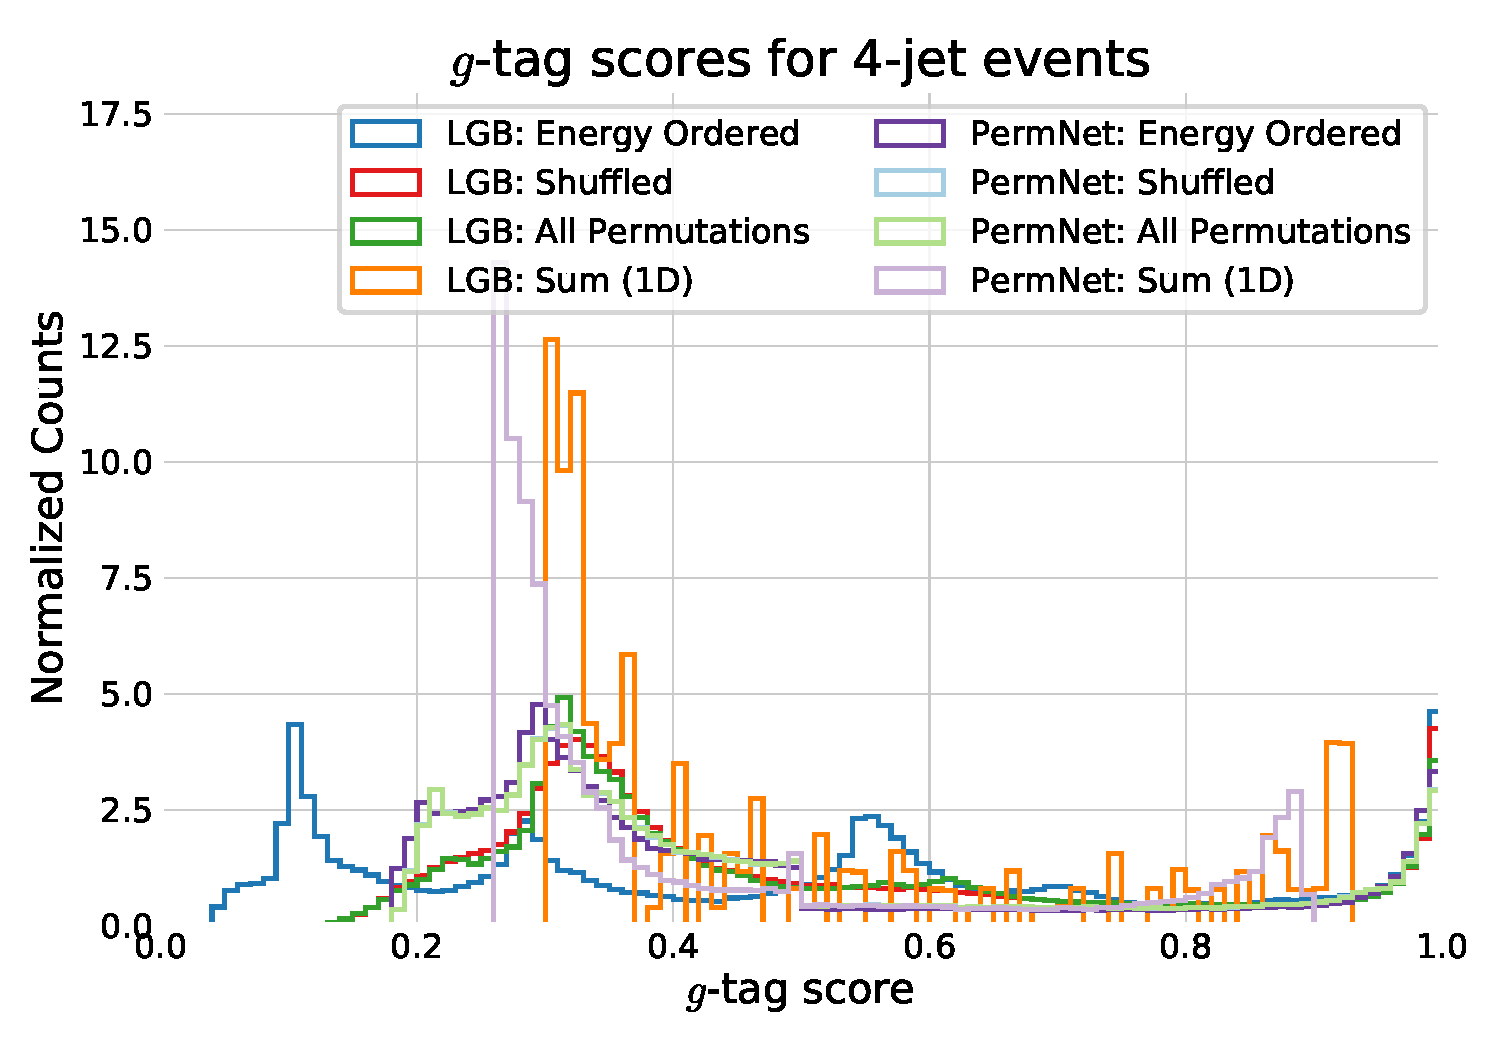
\includegraphics[width=0.95\textwidth, trim=10 10 10 40, clip]{figures/quarks/gtag_y_pred_4_jet_hist-down_sample=1.00-ML_vars=vertex-selection=b-ejet_min=4-n_iter_RS_lgb=99-n_iter_RS_xgb=9-cdot_cut=0.90-version=19.pdf}
  \caption[g-tag scores in 4-jet events]
          {
            Histogram of g-tag scores (model prediction) in 4-jet events for \textcolor{blue}{XGB: Energy Ordered} in blue, \textcolor{red}{XGB: Shuffled} in red, \textcolor{green}{XGB: All Permutations} in green, \textcolor{orange}{XGB: Sum 1D} in orange, \textcolor{purple}{PermNet: Energy Ordered} in purple, \textcolor{light-blue}{PermNet: Shuffled} in light-blue, \textcolor{light-green}{PermNet: All Permutations} in light-green, \textcolor{light-purple}{PermNet: Sum 1D} in light-purple.  Here XGB and PermNet are the two different type of models and \q{Energy Ordered}, \q{Shuffled}, \q{All Permutations}, and \q{Sum 1D} are the different methods used for making the input data permutation invariant.  
          }   
  \label{fig:q:gtag_scores_4j}
\end{figure}


\begin{figure}
  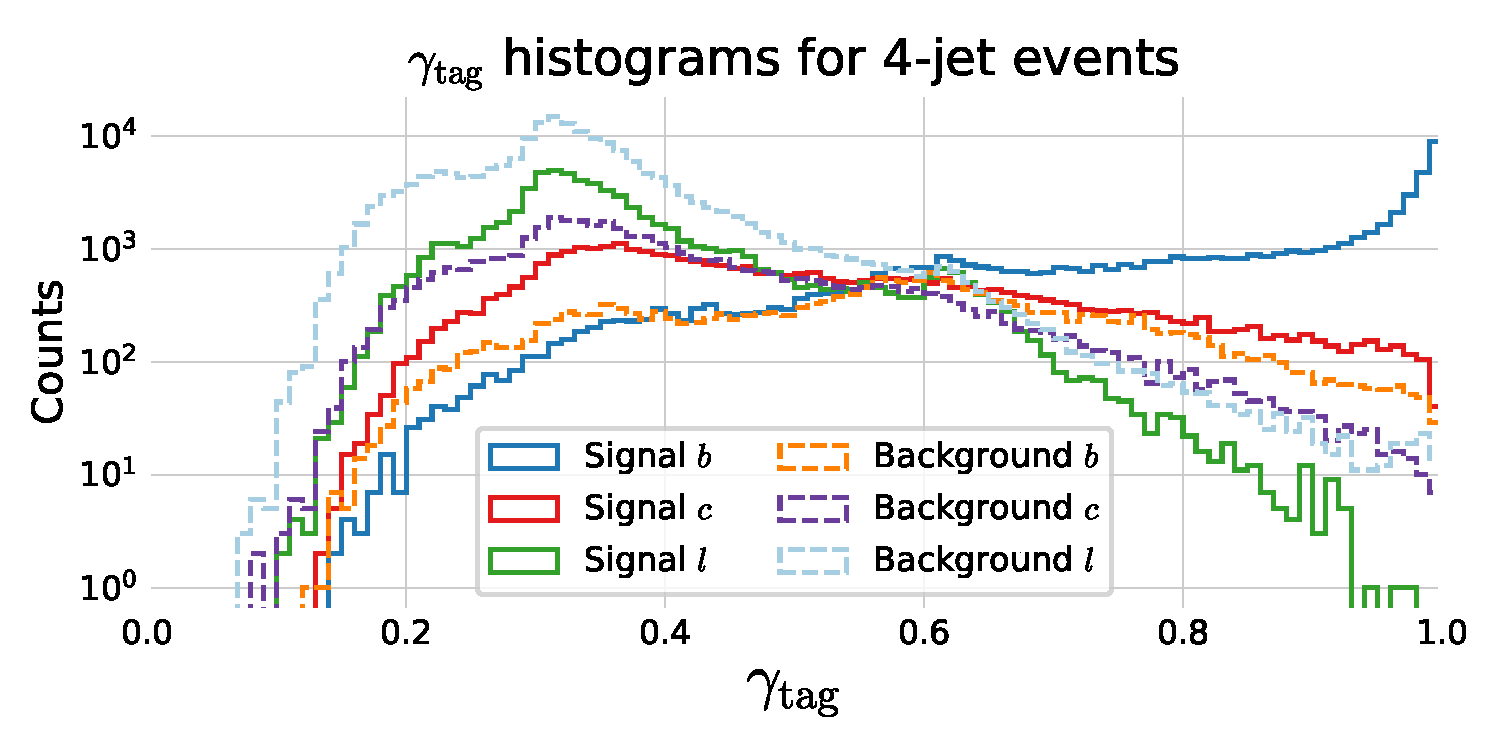
\includegraphics[width=0.95\textwidth, trim=10 10 10 40, clip]{figures/quarks/gtag-histogram-sigbkg-down_sample=1.00-ML_vars=vertex-selection=b-ejet_min=4-n_iter_RS_lgb=99-n_iter_RS_xgb=9-cdot_cut=0.90-version=19-njet=4.pdf}
  \caption[g-tag scores in 4-jet events for signal and background]
          {Histogram of g-tag scores (model prediction) from the XGB-model in 4-jet events for \textcolor{blue}{b signal} in blue, \textcolor{red}{c signal} in red, \textcolor{green}{l signal} in green, \textcolor{orange}{b background} in orange, \textcolor{purple}{c background} in purple, \textcolor{light-blue}{l background} in light-blue.
          } 
  \label{fig:q:gtag_scores_4j_sig_bkg}
\end{figure}





\begin{figure}
  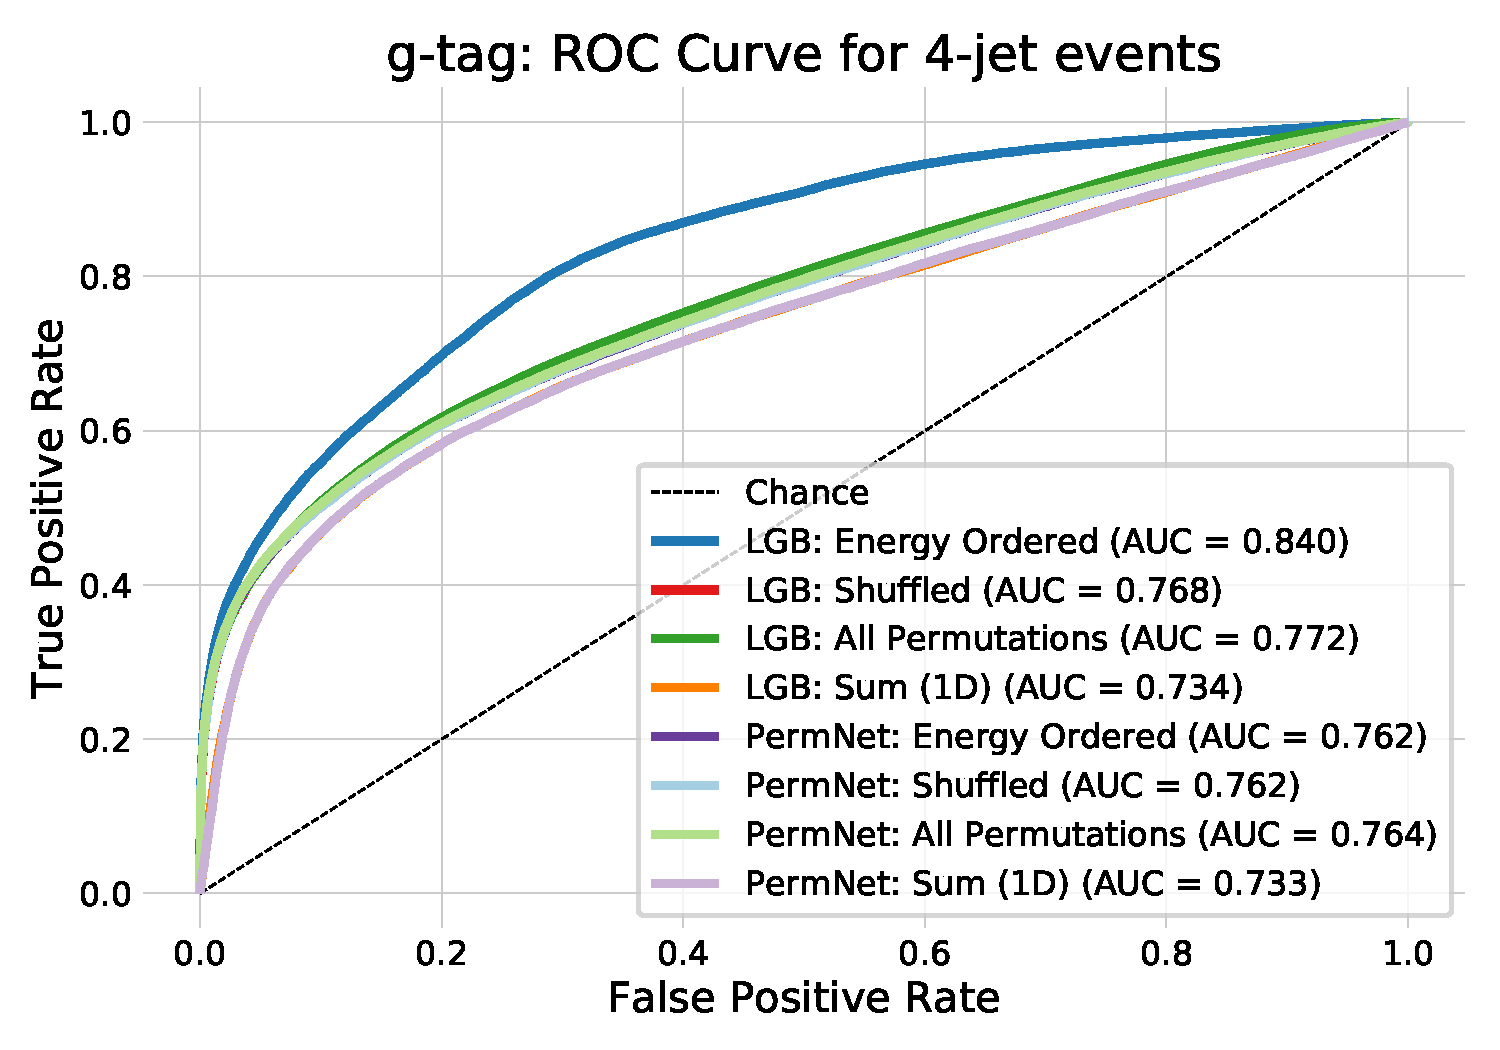
\includegraphics[width=0.95\textwidth, trim=10 10 10 40, clip]{figures/quarks/gtag_ROC_4_jet-down_sample=1.00-ML_vars=vertex-selection=b-ejet_min=4-n_iter_RS_lgb=99-n_iter_RS_xgb=9-cdot_cut=0.90-version=19.pdf}
  \caption[ROC curve for g-tag in 4-jet events]
          {ROC curve of the eight g-tag models in 4-jet events. First one in dashed black is the ROC curve that you get by random chance. The colors are the same as in \figref{fig:q:gtag_scores_4j} and in the legend also the Area Under the ROC curve (AUC) is shown. 
          Notice that the XGB model which uses the energy ordered data produced the best model, however, this model is not permutation invariant. Of the permutation invariant models (the rest), the XGB model trained on all permutations of the b-tags performs highest. The lowest performing models are the two models trained only on the 1-dimensional sum of b-tags, as expected, however, still with a better performance than expected by the author.  
          } 
  \label{fig:q:roc_gtag_4j}
\end{figure}





\begin{figure}
  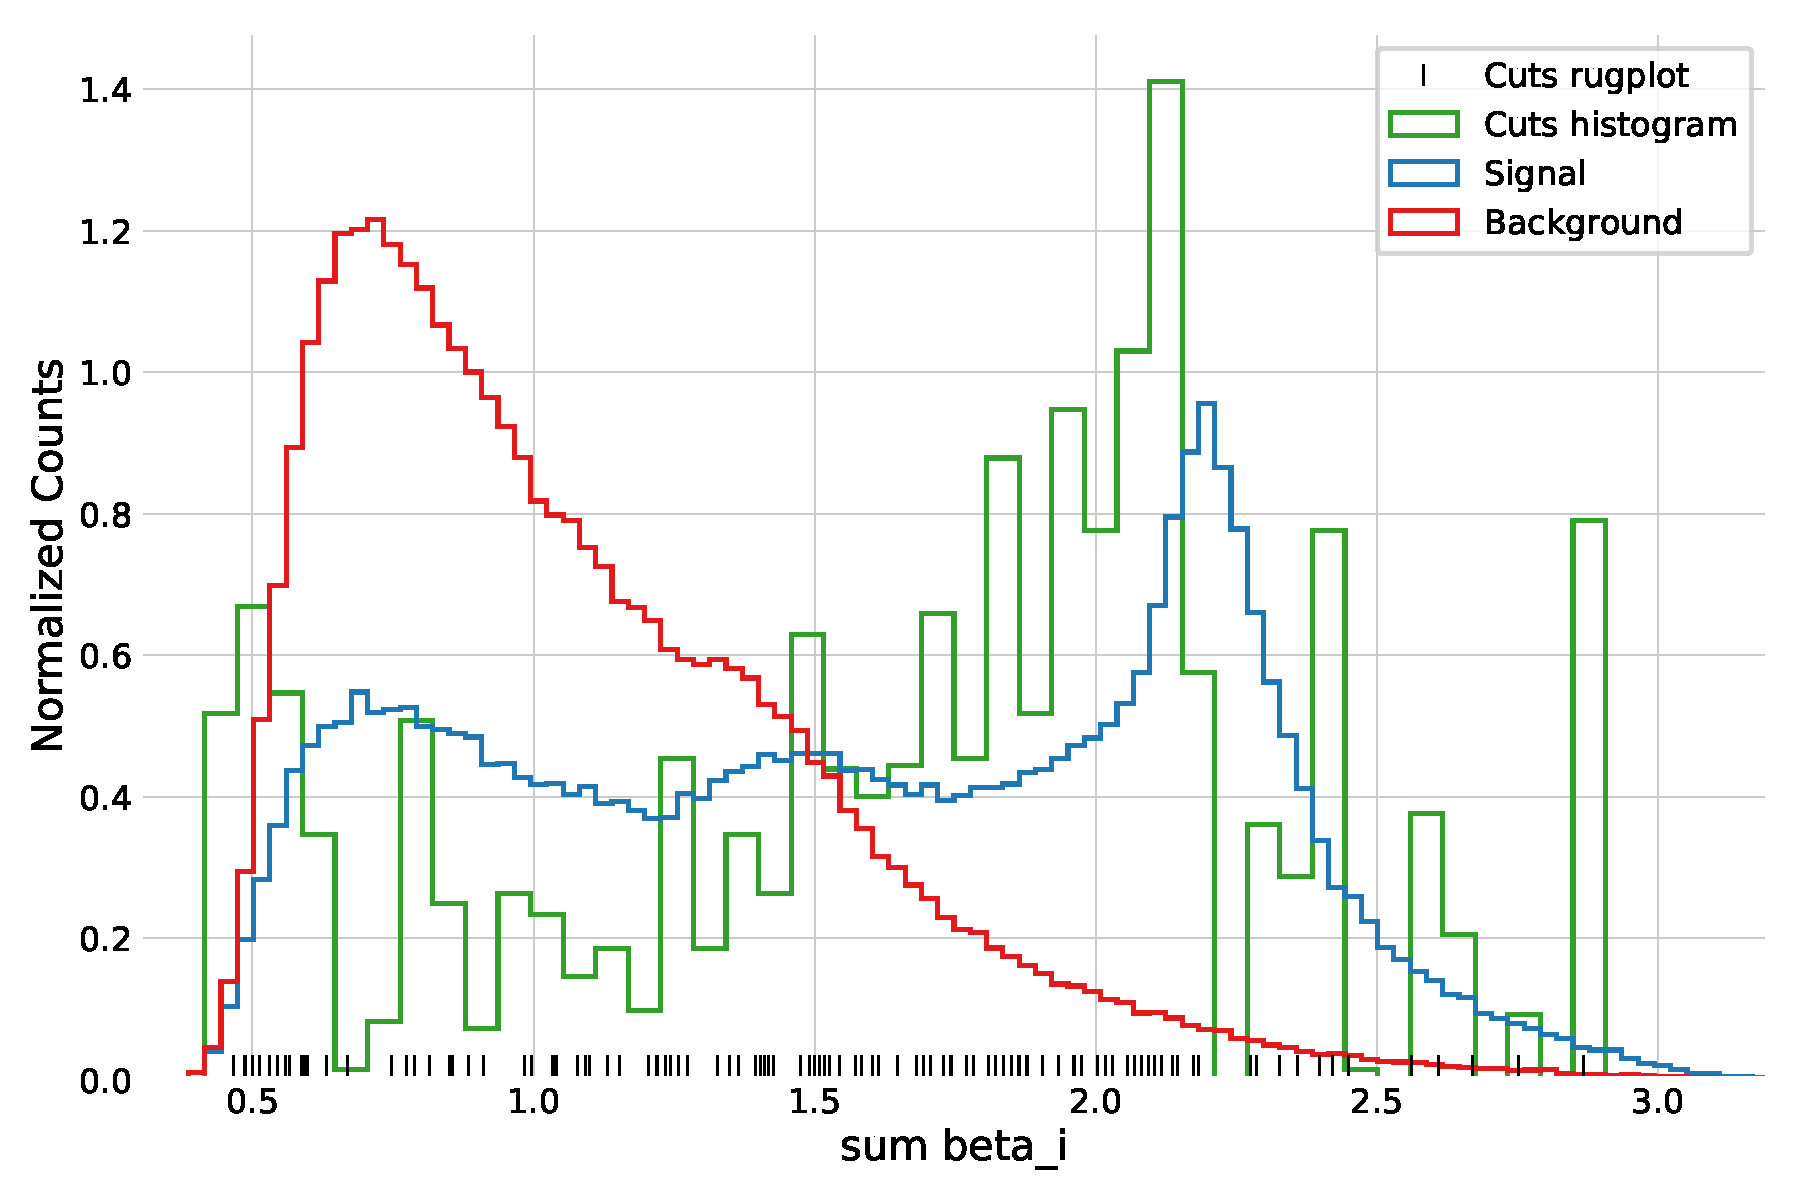
\includegraphics[width=0.95\textwidth, trim=10 10 10 20, clip]{figures/quarks/gtag_sum_method_njet=4-down_sample=1.00-ML_vars=vertex-selection=b-ejet_min=4-n_iter_RS_lgb=99-n_iter_RS_xgb=9-cdot_cut=0.90-version=19.pdf}
  \caption[1D Sum Model Cuts for 4-jets]
          {Histogram of the distribution of \textcolor{blue}{signal} in blue and \textcolor{red}{background} in red for 1-dimensional sum of b-tags training data. A histogram of the \textcolor{green}{cut values} from the XGB model trained on this data is shown in green together with a rug plot of the cut values in black. Notice how most of the cuts match up with the signal peak at around a $\sum \beta_i \sim 2.1$, however, there are also quite a lot of cuts around $\sum \beta_i \sim 0.5$.
          } 
  \label{fig:q:1d_sum_model_cuts_4j}
\end{figure}


\begin{figure}
  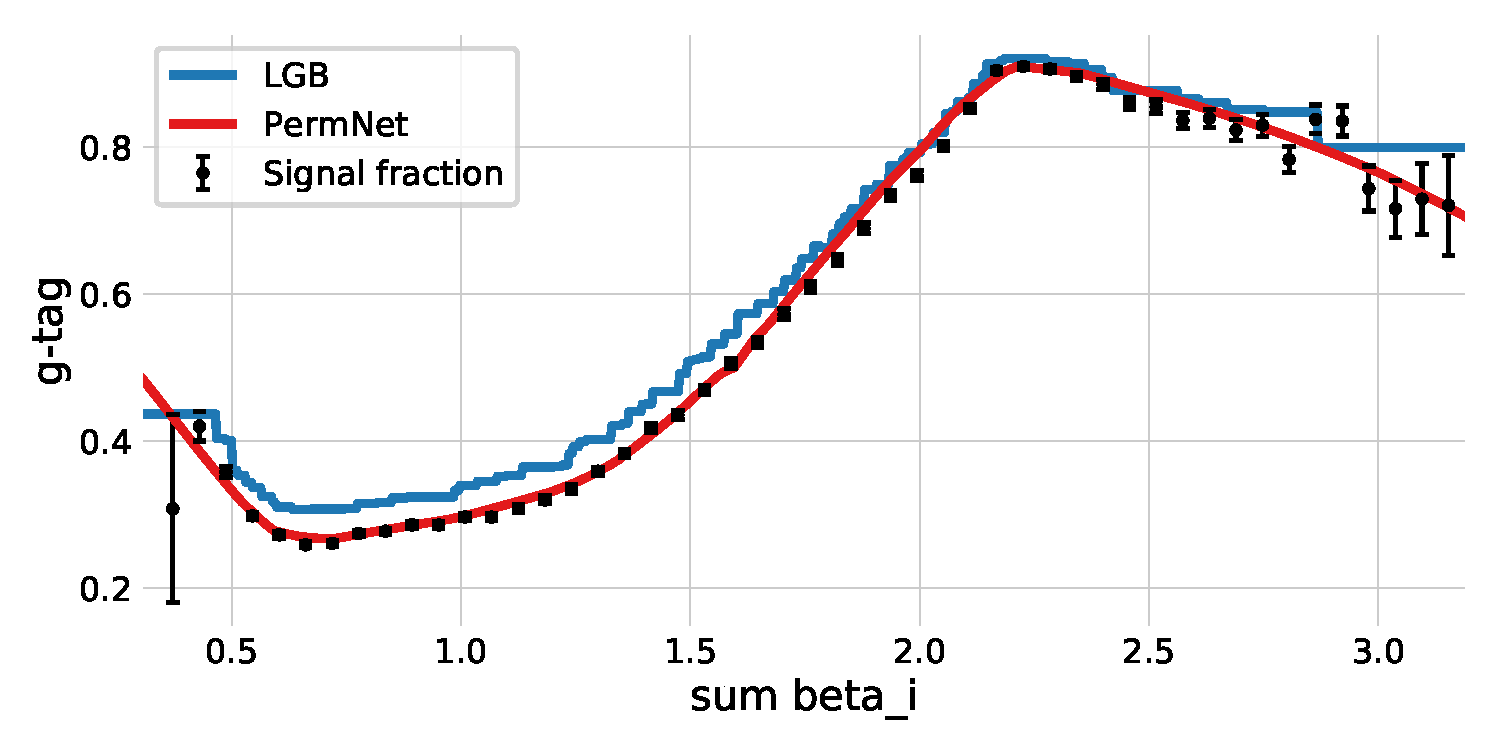
\includegraphics[width=0.95\textwidth, trim=10 10 10 20, clip]{figures/quarks/gtag_sum_models_njet=4-down_sample=1.00-ML_vars=vertex-selection=b-ejet_min=4-n_iter_RS_lgb=99-n_iter_RS_xgb=9-cdot_cut=0.90-version=19.pdf}
  \caption[1D Sum Models Predictions and Signal Fraction for 4-jets]
          {Plot of the (1D) g-tag scores as a function of $\sum \beta_i$ for the \textcolor{blue}{XGB} model in blue and the \textcolor{red}{PermNet} model in red. Here the g-tag scores are just the models' output values when input a uniformly spaced grid of $\sum \beta_i$ values between 0 and 4. The signal fraction (based on the signal and background histograms in \figref{fig:q:1d_sum_model_cuts_4j}) is plotted as black error bars where the size of the error bars is based on the propagated uncertainties of the signal and background histogram assuming Poissonian statistics. Notice how both models capture the overall trend of the signal fraction with the PermNet being particularly close. 
          } 
  \label{fig:q:1d_sum_models_signal_fraction_4j}
\end{figure}








\begin{figure}
  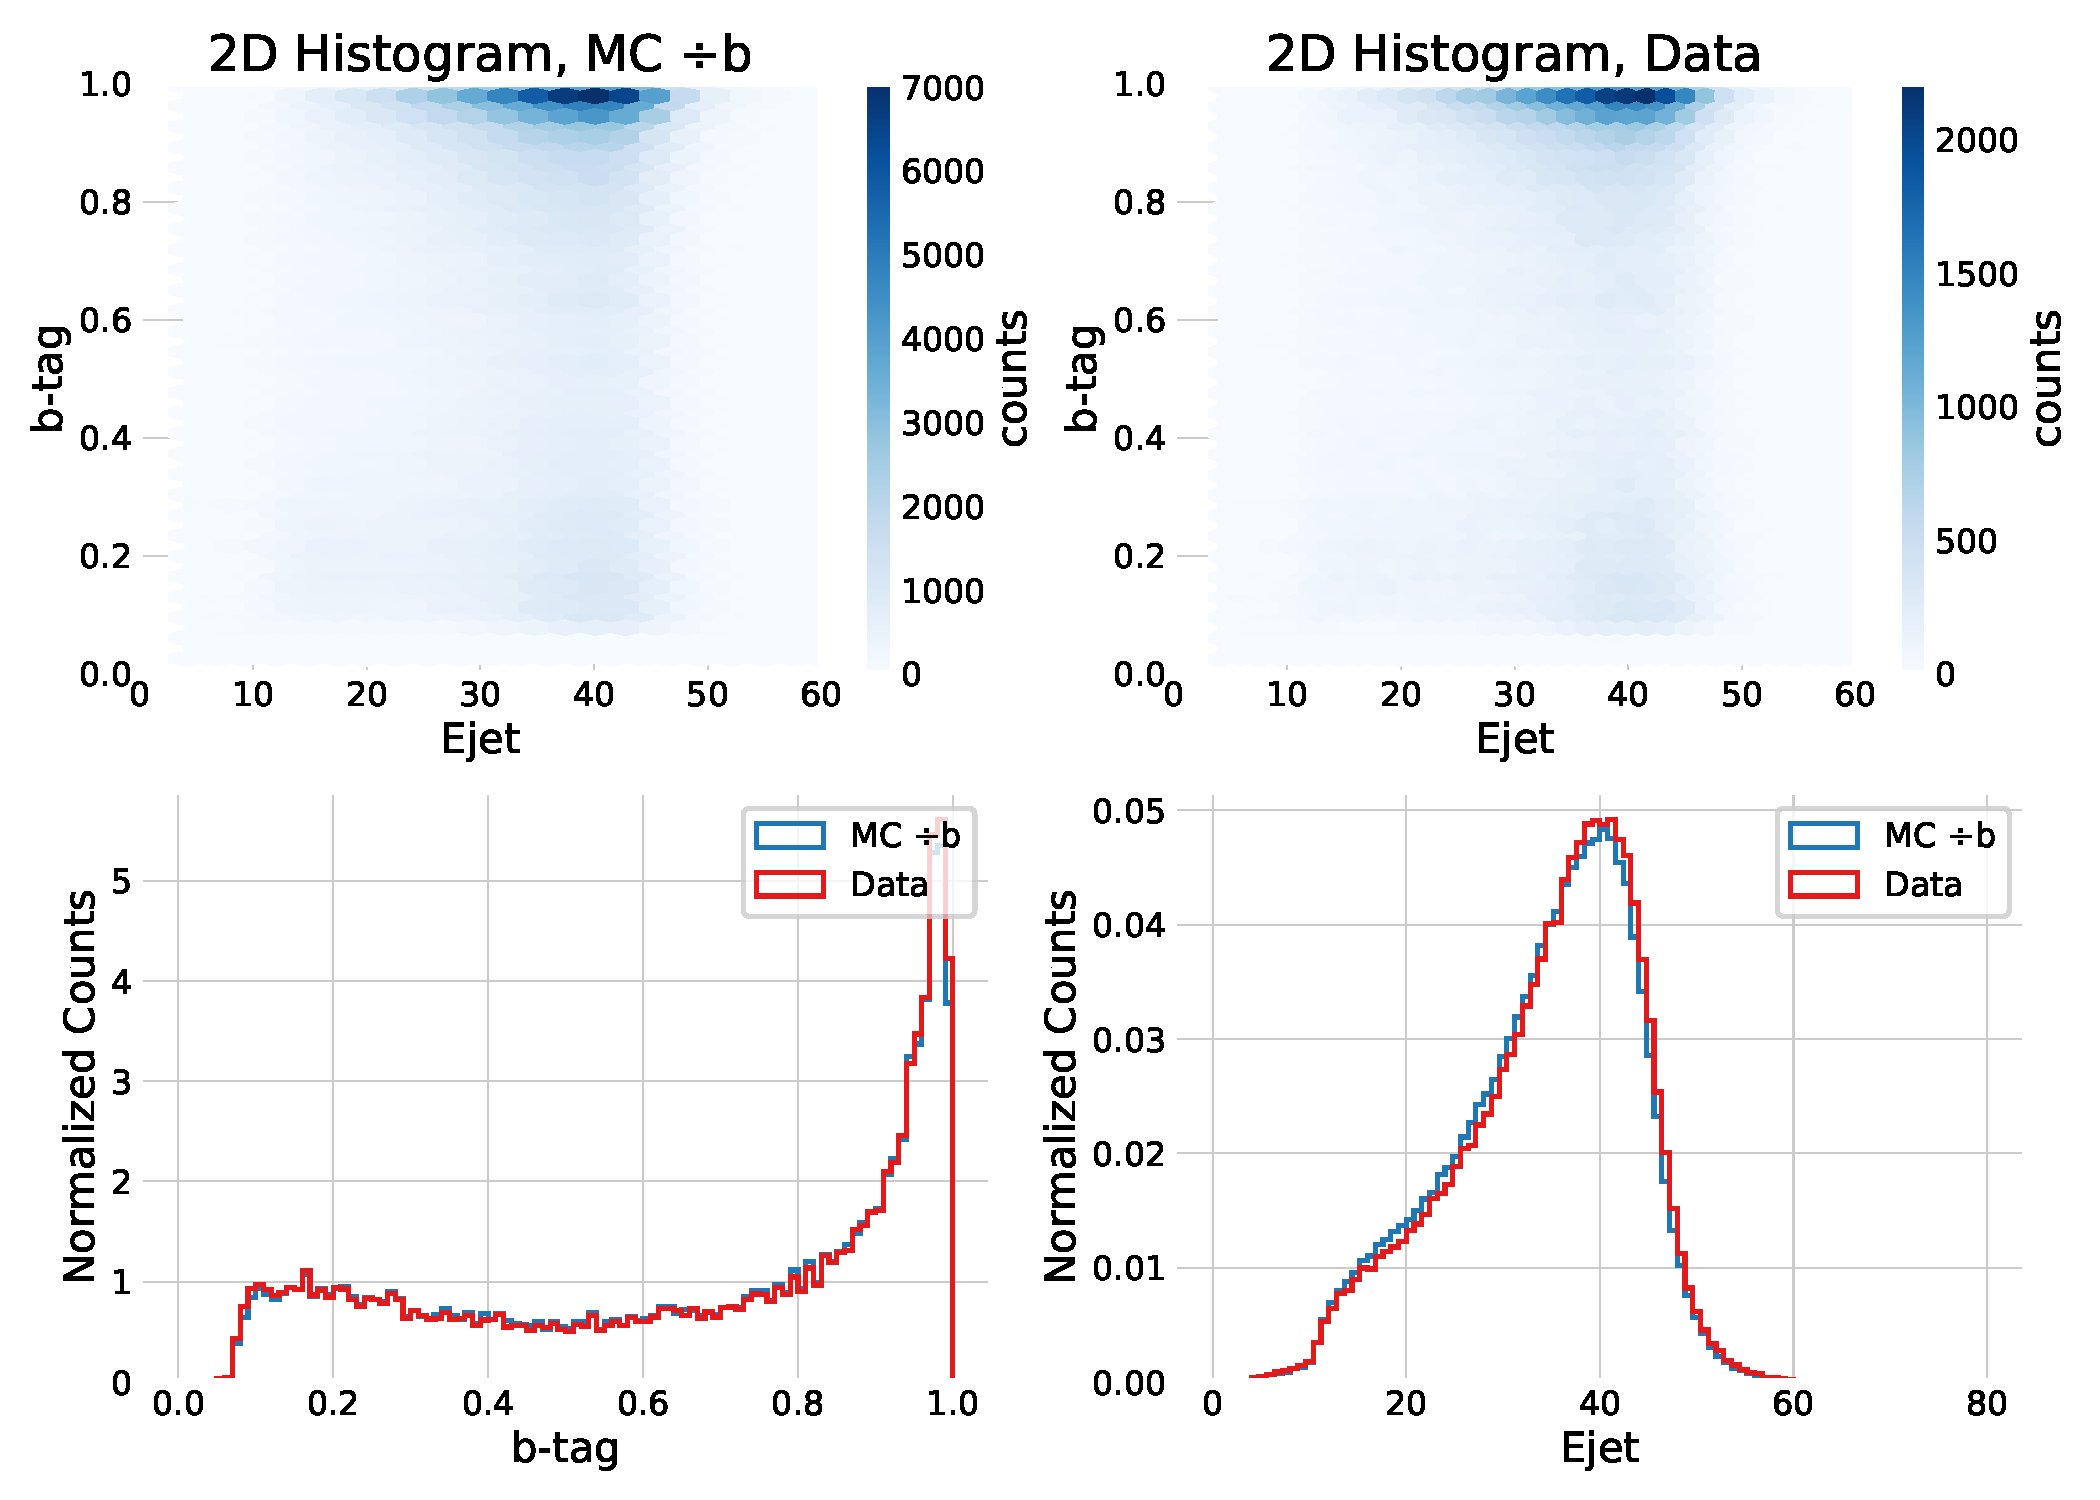
\includegraphics[width=0.95\textwidth, trim=0 0 0 40, clip]{figures/quarks/2d-histograms-ejet-btag-comparison-down_sample=1.00-ML_vars=vertex-selection=b-ejet_min=4-n_iter_RS_lgb=99-n_iter_RS_xgb=9-cdot_cut=0.90-version=19-njet=3.pdf}
  \caption[Monte Carlo -- Data bias for b-tags and jet energy]
          {Comparison of the b-tag and jet energy (\code{Ejet}) distributions for Monte Carlo (MC) versus data. In the top row the 2D-distributions are shown for MC on the left (without the extra MCb samples) and data on the right. In the bottom row the 1D marginal distrubtions are shown for the b-tag and the jet energy with \textcolor{red}{data} in red and \textcolor{blue}{Monte Carlo} ones in blue. Notice the the almost identical distributions in b-tag. 
          } 
  \label{fig:q:btag_Ejet_comparison}
\end{figure}

\begin{figure}
  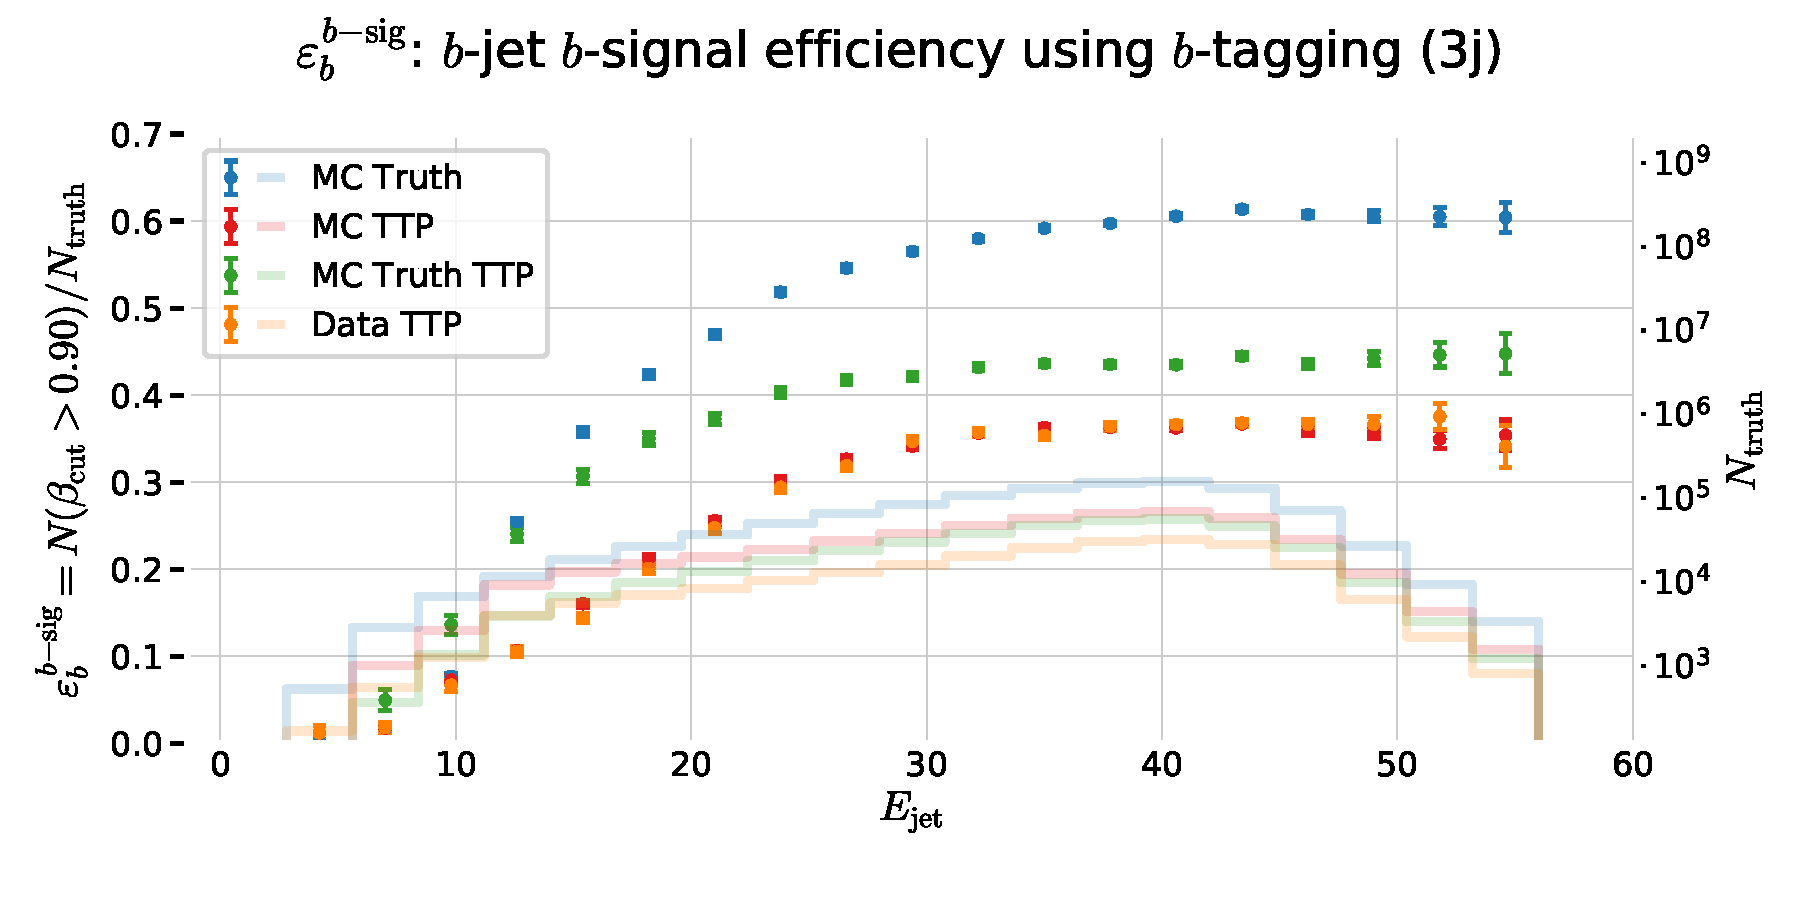
\includegraphics[width=0.95\textwidth, trim=0 0 0 40, clip]{figures/quarks/eff_b_bsig-down_sample=1.00-ML_vars=vertex-selection=b-ejet_min=4-n_iter_RS_lgb=99-n_iter_RS_xgb=9-cdot_cut=0.90-version=19.pdf}
  \caption[b-Tagging Efficiency $\varepsilon_b^{b\mathrm{-sig}}$ as a function of jet energy]
          {Efficiency of the b-tags for b-jets in the b-signal region for 3-jet events, $\varepsilon_b^{b\mathrm{-sig}}$, as a function of jet energy \code{Ejet}. The b-signal region is defined as $\beta > 0.9$. In the plot the efficiencies are shown for \textcolor{blue}{MC Truth} in blue, \textcolor{red}{MC TTP} in red, \textcolor{green}{MC Truth TTP} in green, and \textcolor{orange}{Data TTP} in orange. The efficiencies (the errorbars) can be read off on the left y-axis and the counts (histograms) on the right y-axis. The abbreviation TTP is short for \q{Tag, Tag, Probe} where two jets in a event are used as tags and the probe is then used for further analysis. Notice how both MC TTP and Data TTP follow each other closely.  
          } 
  \label{fig:q:effiency_btag_bjet_bsig}
\end{figure}


\begin{figure}
  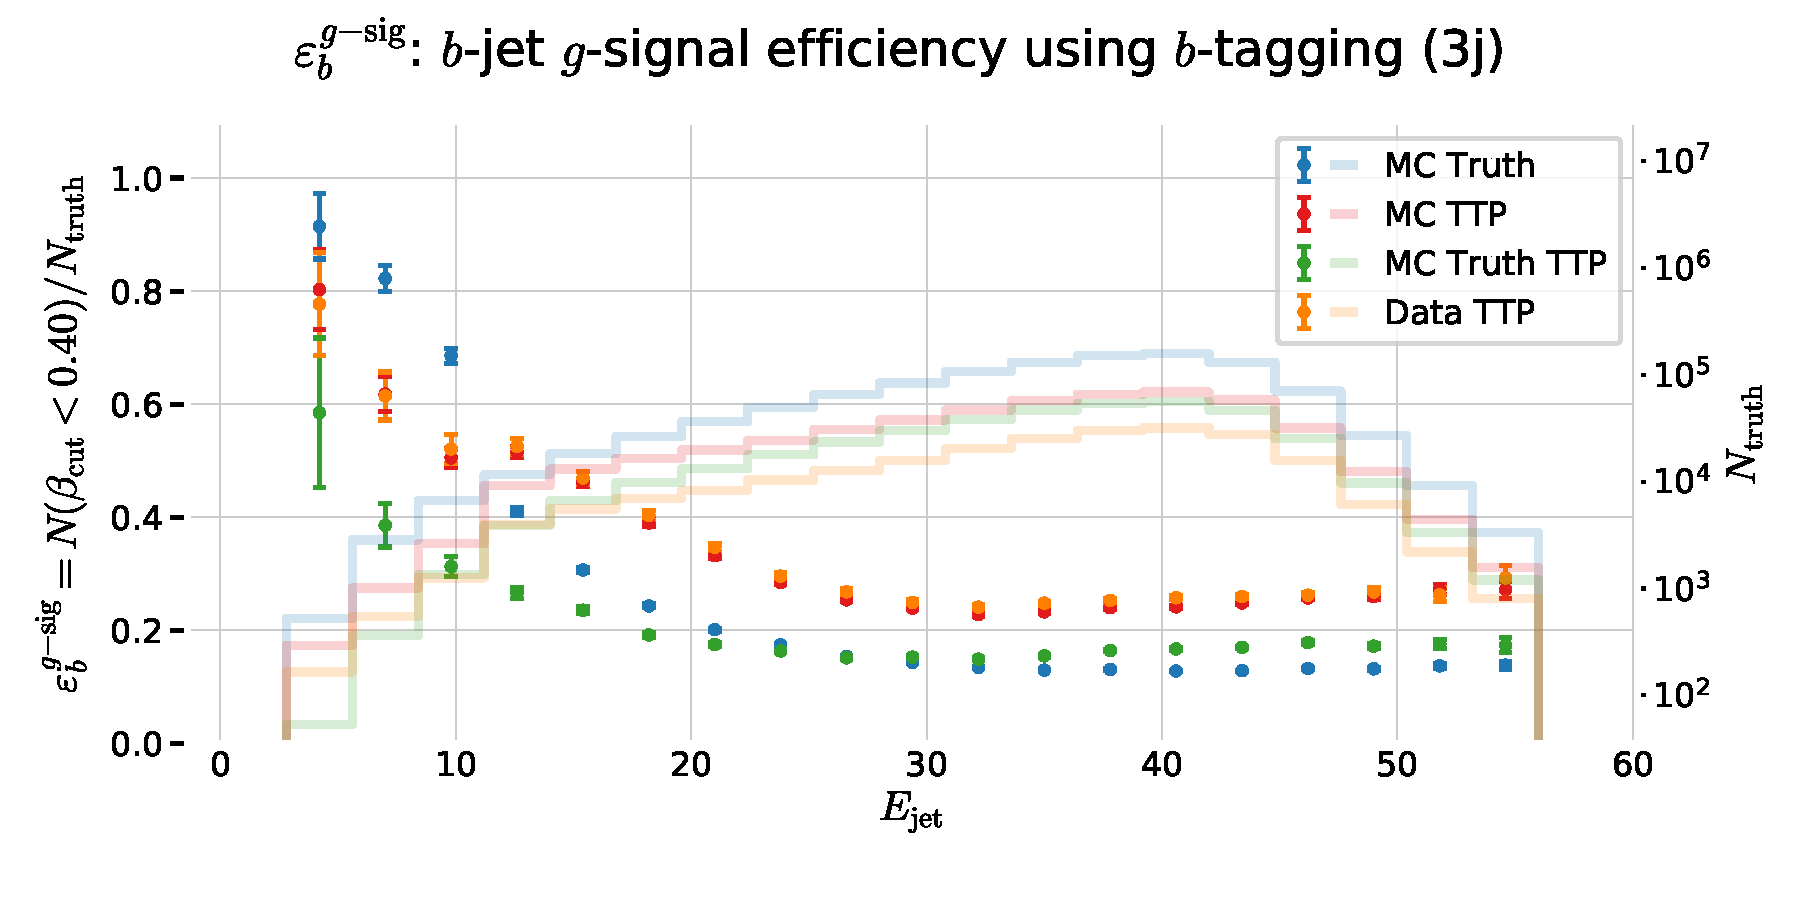
\includegraphics[width=0.95\textwidth, trim=0 0 0 40, clip]{figures/quarks/eff_b_gsig-down_sample=1.00-ML_vars=vertex-selection=b-ejet_min=4-n_iter_RS_lgb=99-n_iter_RS_xgb=9-cdot_cut=0.90-version=19.pdf}
  \caption[b-Tagging Efficiency $\varepsilon_b^{g\mathrm{-sig}}$ as a function of jet energy]
          {Efficiency of the b-tags for b-jets in the g-signal region for 3-jet events, $\varepsilon_b^{g\mathrm{-sig}}$, as a function of jet energy \code{Ejet}. The g-signal region is defined as $\beta < 0.4$. In the plot the efficiencies are shown for \textcolor{blue}{MC Truth} in blue, \textcolor{red}{MC TTP} in red, \textcolor{green}{MC Truth TTP} in green, and \textcolor{orange}{Data TTP} in orange. The efficiencies (the errorbars) can be read off on the left y-axis and the counts (histograms) on the right y-axis. The abbreviation TTP is short for \q{Tag, Tag, Probe} where two jets in a event are used as tags and the probe is then used for further analysis. Notice how both MC TTP and Data TTP follow each other closely.  
          } 
  \label{fig:q:effiency_btag_bjet_gsig}
\end{figure}


\begin{figure}
  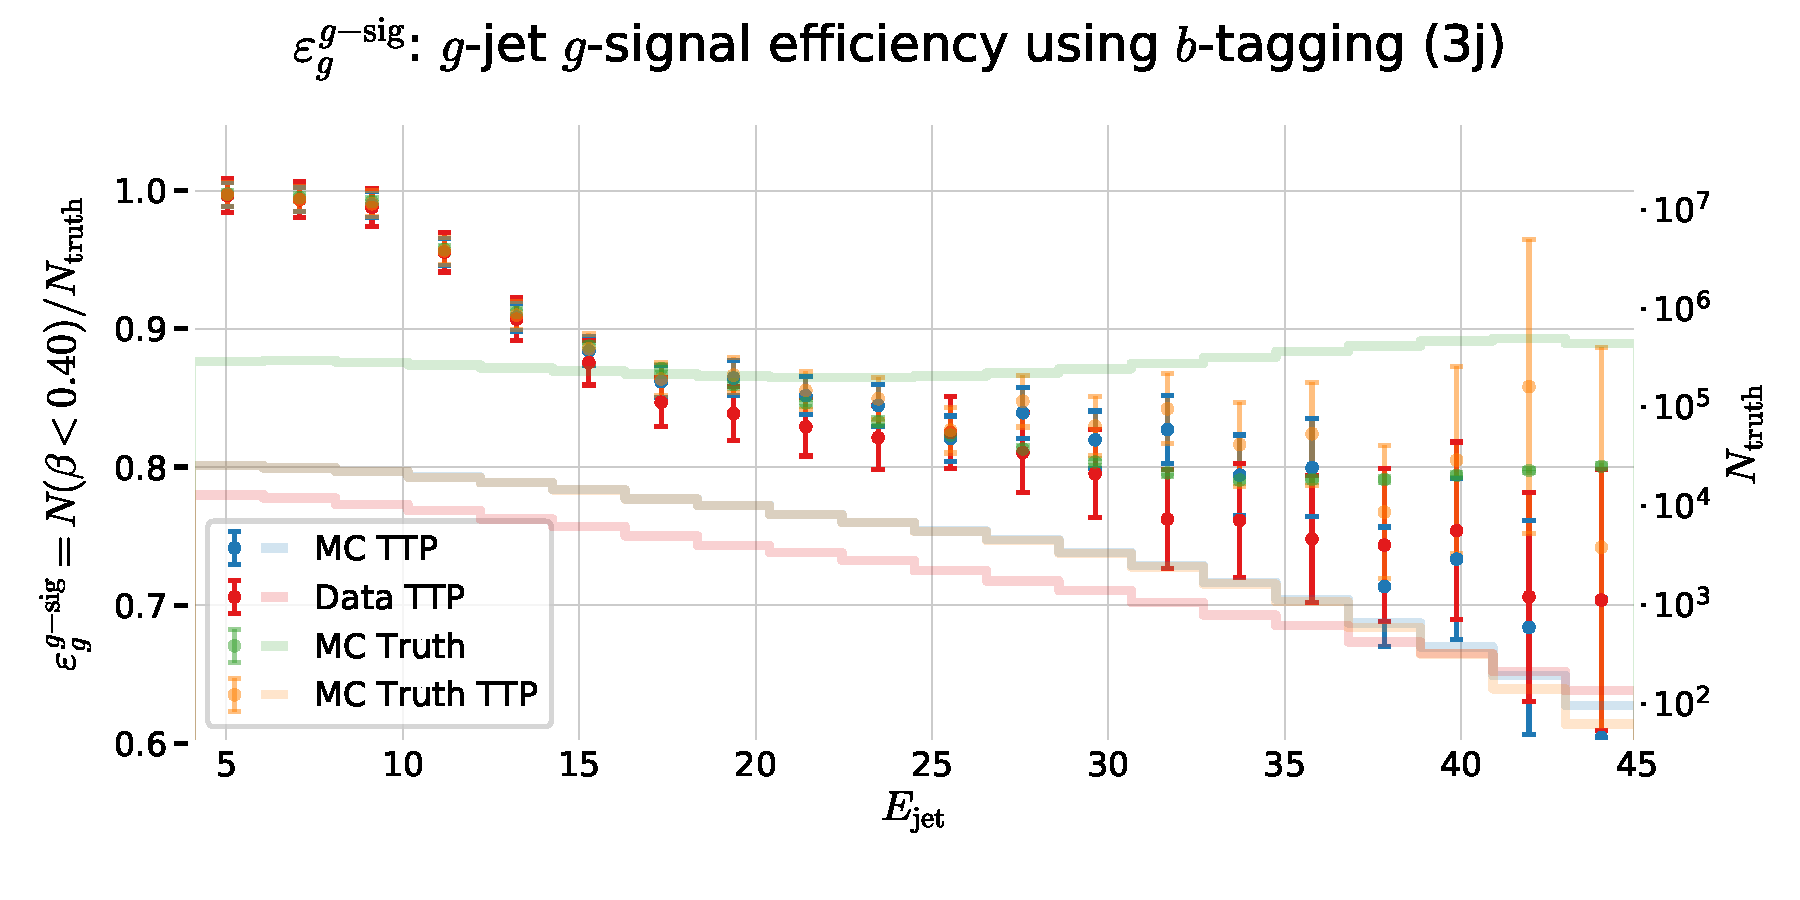
\includegraphics[width=0.95\textwidth, trim=0 0 0 40, clip]{figures/quarks/eff_g_gsig-down_sample=1.00-ML_vars=vertex-selection=b-ejet_min=4-n_iter_RS_lgb=99-n_iter_RS_xgb=9-cdot_cut=0.90-version=19.pdf}
  \caption[b-Tagging Efficiency $\varepsilon_g^{g\mathrm{-sig}}$ as a function of jet energy]
          {Efficiency of the b-tags for g-jets in the g-signal region for 3-jet events, $\varepsilon_g^{g\mathrm{-sig}}$, as a function of jet energy \code{Ejet}. The g-signal region is defined as $\beta < 0.4$. In the plot the efficiencies are shown for \textcolor{blue}{MC Truth} in blue, \textcolor{red}{MC TTP} in red, \textcolor{green}{MC Truth TTP} in green, and \textcolor{orange}{Data TTP} in orange. The efficiencies (the errorbars) can be read off on the left y-axis and the counts (histograms) on the right y-axis. The abbreviation TTP is short for \q{Tag, Tag, Probe} where two jets in a event are used as tags and the probe is then used for further analysis. Notice how both MC TTP and Data TTP follow each other closely.  
          } 
  \label{fig:q:effiency_btag_gjet_gsig}
\end{figure}

\begin{figure}
  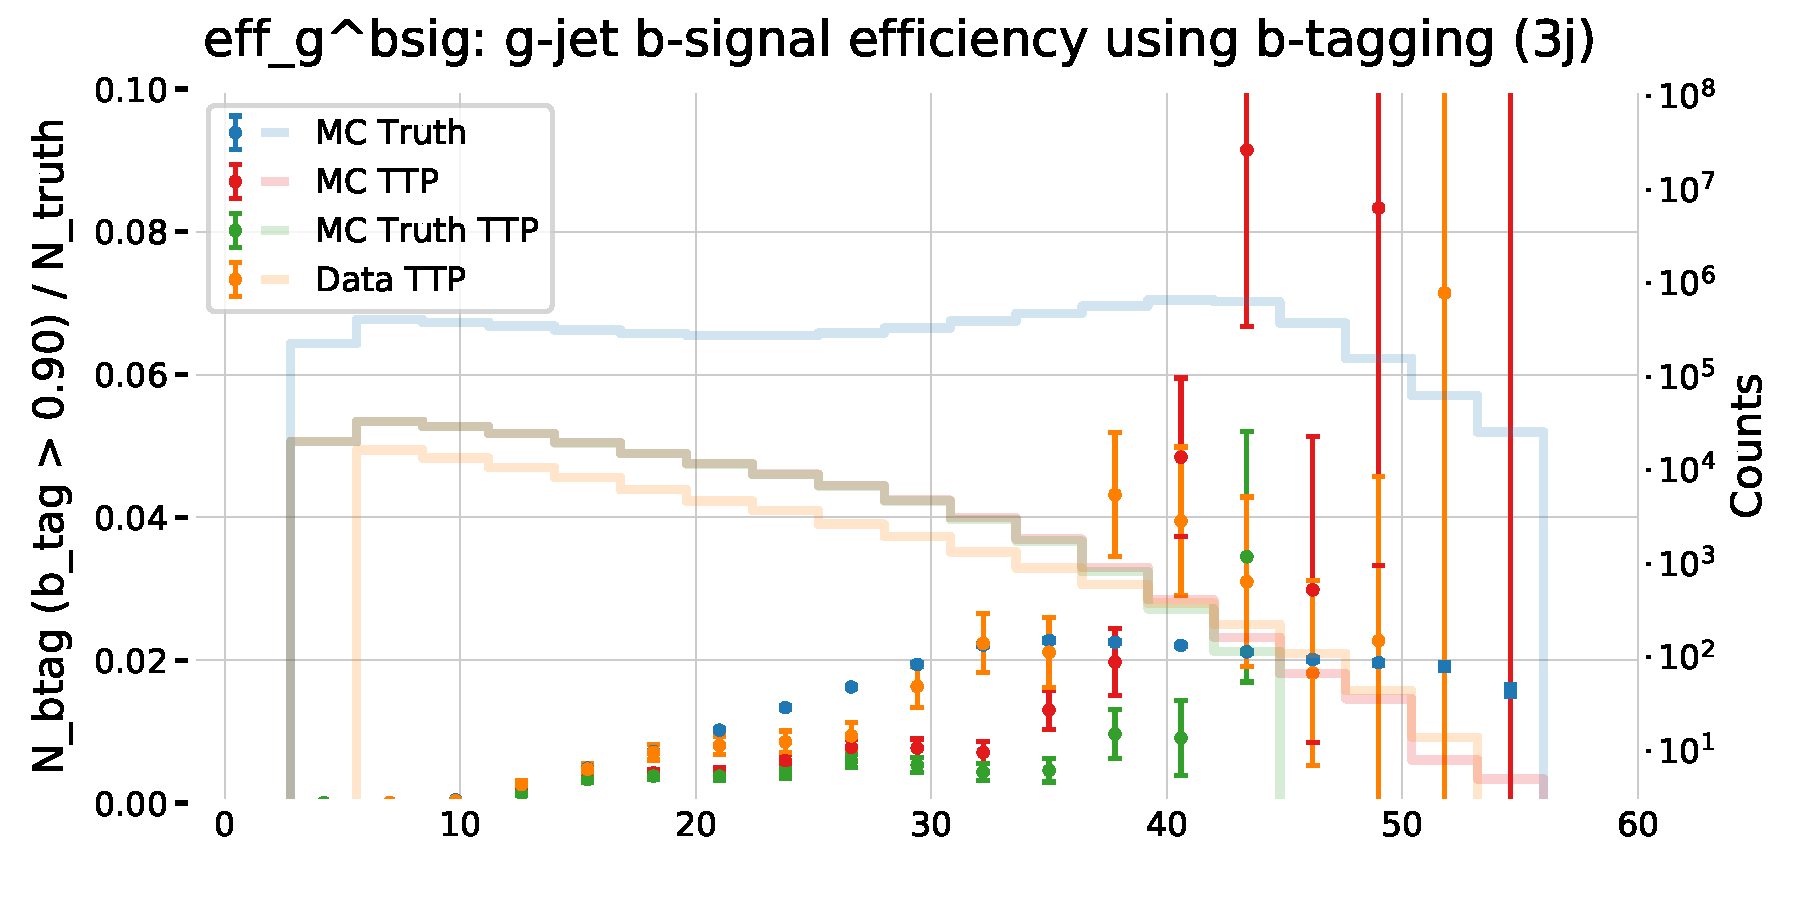
\includegraphics[width=0.95\textwidth, trim=0 0 0 30, clip]{figures/quarks/eff_g_bsig-down_sample=1.00-ML_vars=vertex-selection=b-ejet_min=4-n_iter_RS_lgb=99-n_iter_RS_xgb=9-cdot_cut=0.90-version=19.pdf}
  \caption[b-Tagging Efficiency $\varepsilon_g^{b\mathrm{-sig}}$ as a function of jet energy]
          {Efficiency of the b-tags for g-jets in the b-signal region for 3-jet events, $\varepsilon_g^{b\mathrm{-sig}}$, as a function of jet energy \code{Ejet}. The b-signal region is defined as $\beta > 0.9$. In the plot the efficiencies are shown for \textcolor{blue}{MC Truth} in blue, \textcolor{red}{MC TTP} in red, \textcolor{green}{MC Truth TTP} in green, and \textcolor{orange}{Data TTP} in orange. The efficiencies (the errorbars) can be read off on the left y-axis and the counts (histograms) on the right y-axis. The abbreviation TTP is short for \q{Tag, Tag, Probe} where two jets in a event are used as tags and the probe is then used for further analysis.  
          } 
  \label{fig:q:effiency_btag_gjet_bsig}
\end{figure}


\begin{figure}
  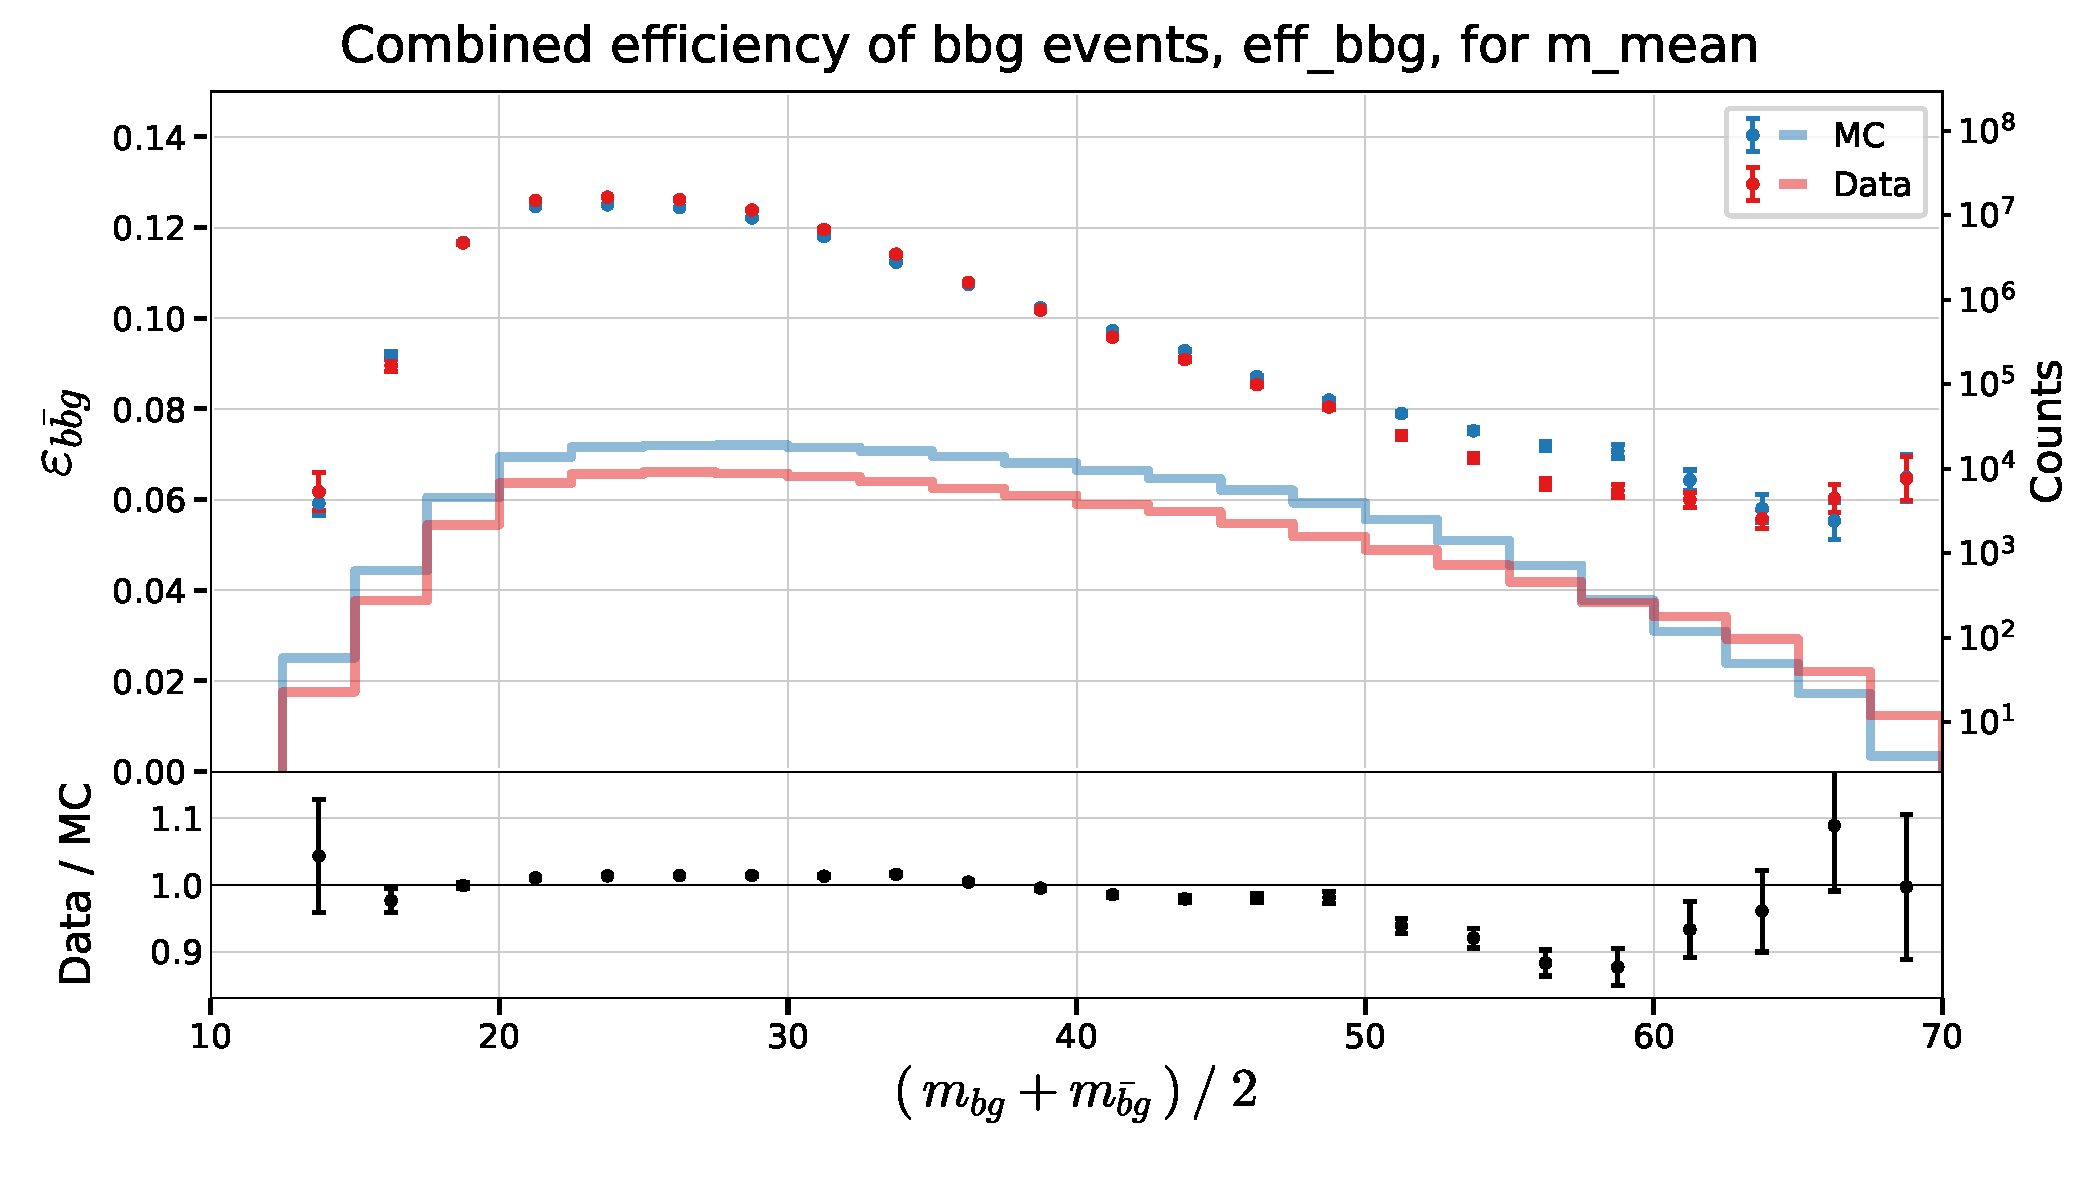
\includegraphics[width=0.95\textwidth, trim=0 0 0 40, clip]{figures/quarks/eff_bbg_m_mean-down_sample=1.00-ML_vars=vertex-selection=b-ejet_min=4-n_iter_RS_lgb=99-n_iter_RS_xgb=9-cdot_cut=0.90-version=19.pdf}
  \caption[g-Tagging proxy efficiency for $b\bar{b}g$-events as function of the mean invariant mass]
          {Proxy efficiency of the g-tags for $b\bar{b}g$ 3-jet events as a function of the mean of the two invariant masses $m_{bg}$ and $m_{\bar{b}g}$. The proxy efficiency $\varepsilon_{b\bar{b}g}$ is measured by finding $b\bar{b}g$-events where $\beta_b > 0.9$, $\beta_{\bar{b}}>0.9$, and $\beta_g < 0.4$. and then calculating  $\varepsilon_{b\bar{b}g} = \varepsilon_b^{b\mathrm{-sig}} \cdot \varepsilon_{\bar{b}}^{b\mathrm{-sig}} \cdot  \varepsilon_g^{g\mathrm{-sig}} $. In the top plot $\varepsilon_{b\bar{b}g}$ is shown for \textcolor{blue}{MC} in blue and \textcolor{red}{Data} in red where the counts in each bin can be read on right y-axis. In the bottom plot the ratio between Data and MC is shown.
          } 
  \label{fig:q:effiency_btag_bbg_m_mean}
\end{figure}


\begin{figure}
  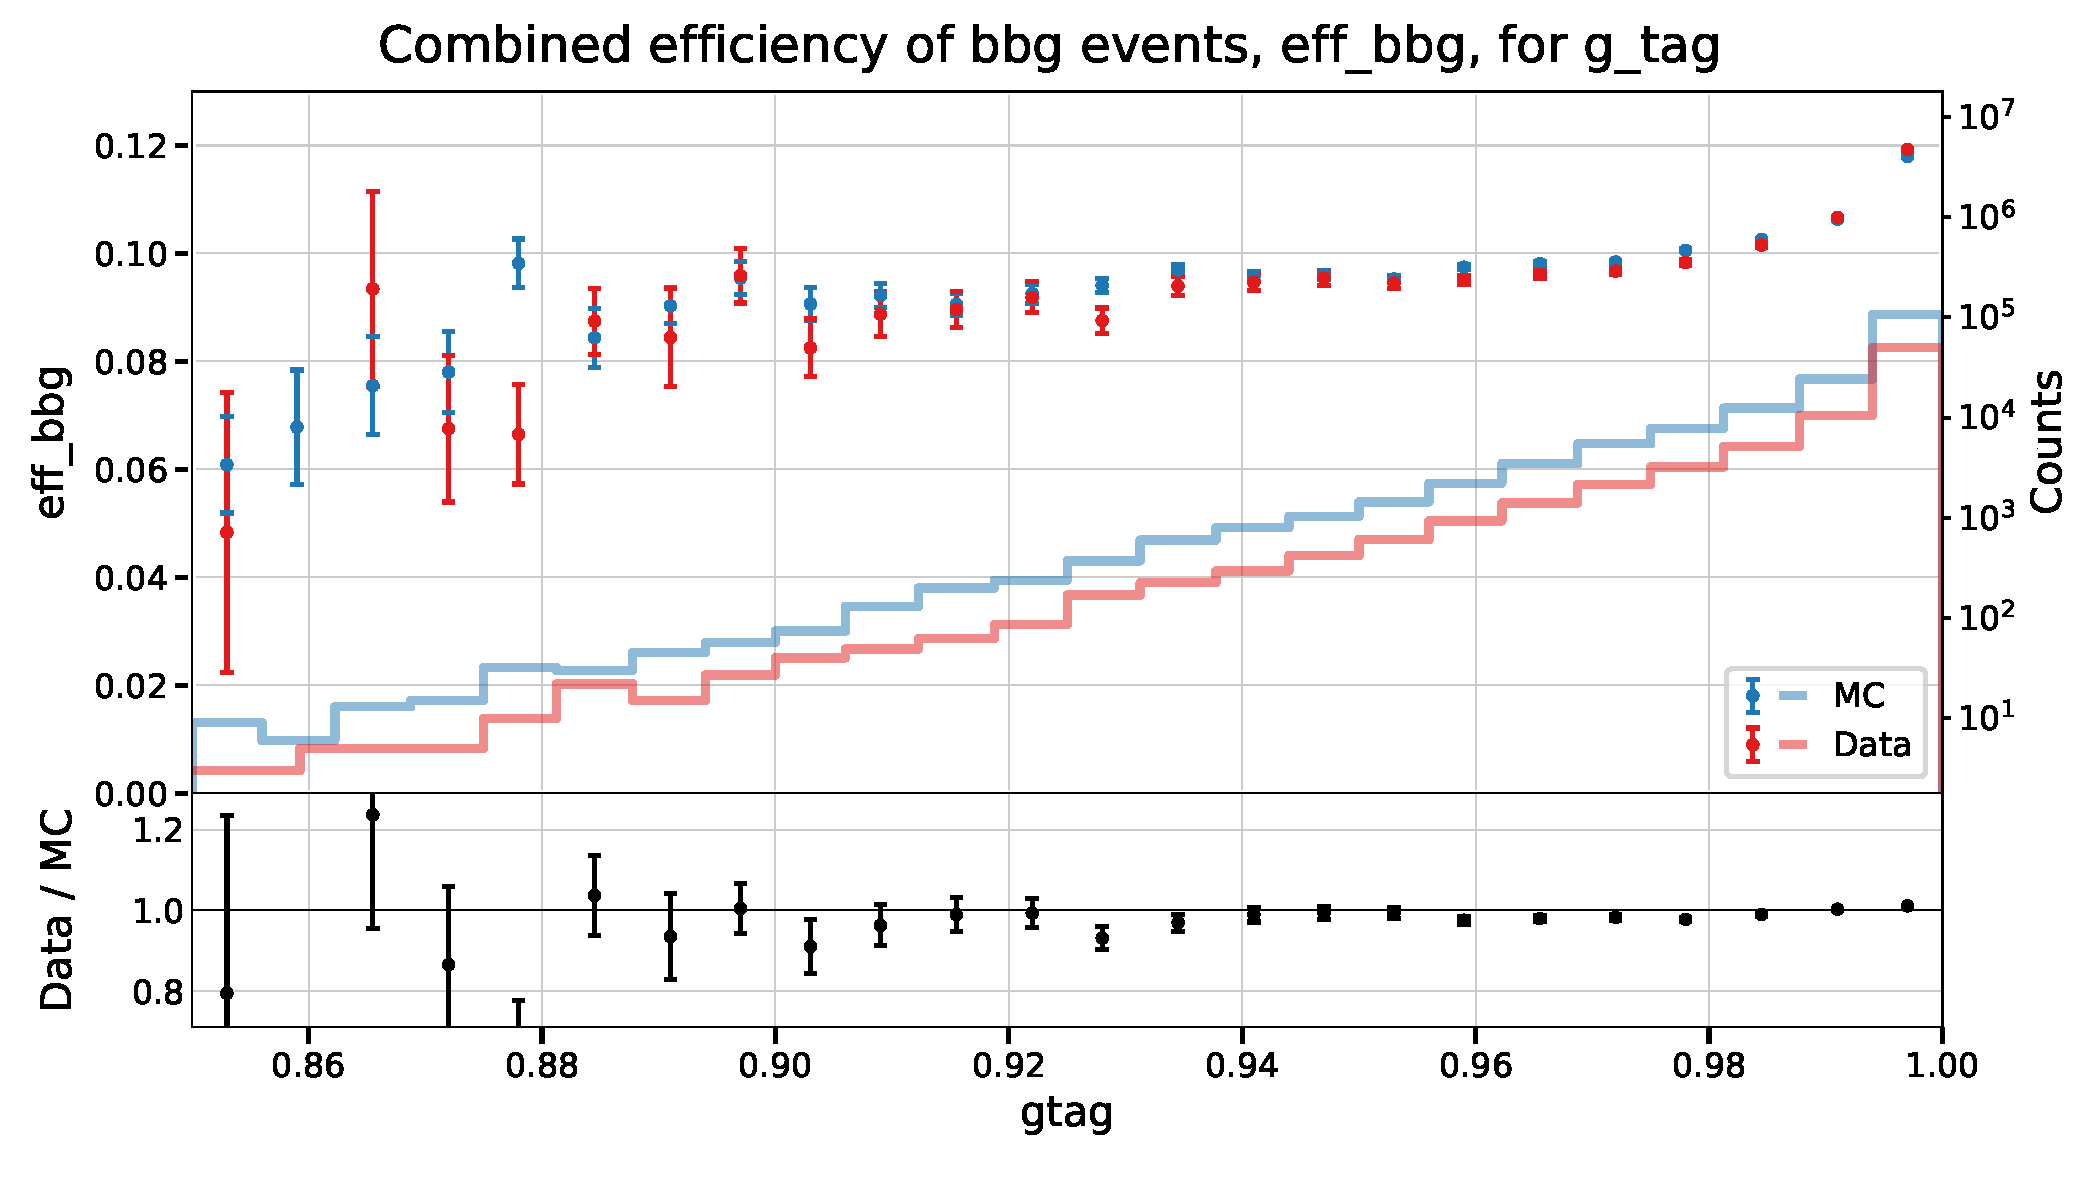
\includegraphics[width=0.95\textwidth, trim=0 0 0 40, clip]{figures/quarks/eff_bbg_gtag-down_sample=1.00-ML_vars=vertex-selection=b-ejet_min=4-n_iter_RS_lgb=99-n_iter_RS_xgb=9-cdot_cut=0.90-version=19.pdf}
  \caption[g-Tagging proxy efficiency for $b\bar{b}g$-events as function of g-tag]
          {Proxy efficiency of the g-tags for $b\bar{b}g$ 3-jet events as a function of the event's g-tag. The proxy efficiency $\varepsilon_{b\bar{b}g}$ is measured by finding $b\bar{b}g$-events where $\beta_b > 0.9$, $\beta_{\bar{b}}>0.9$, and $\beta_g < 0.4$. and then calculating  $\varepsilon_{b\bar{b}g} = \varepsilon_b^{b\mathrm{-sig}} \cdot \varepsilon_{\bar{b}}^{b\mathrm{-sig}} \cdot  \varepsilon_g^{g\mathrm{-sig}} $. In the top plot $\varepsilon_{b\bar{b}g}$ is shown for \textcolor{blue}{MC} in blue and \textcolor{red}{Data} in red where the counts in each bin can be read on right y-axis. In the bottom plot the ratio between Data and MC is shown.
          } 
  \label{fig:q:effiency_btag_bbg_gtag}
\end{figure}



\begin{figure}
  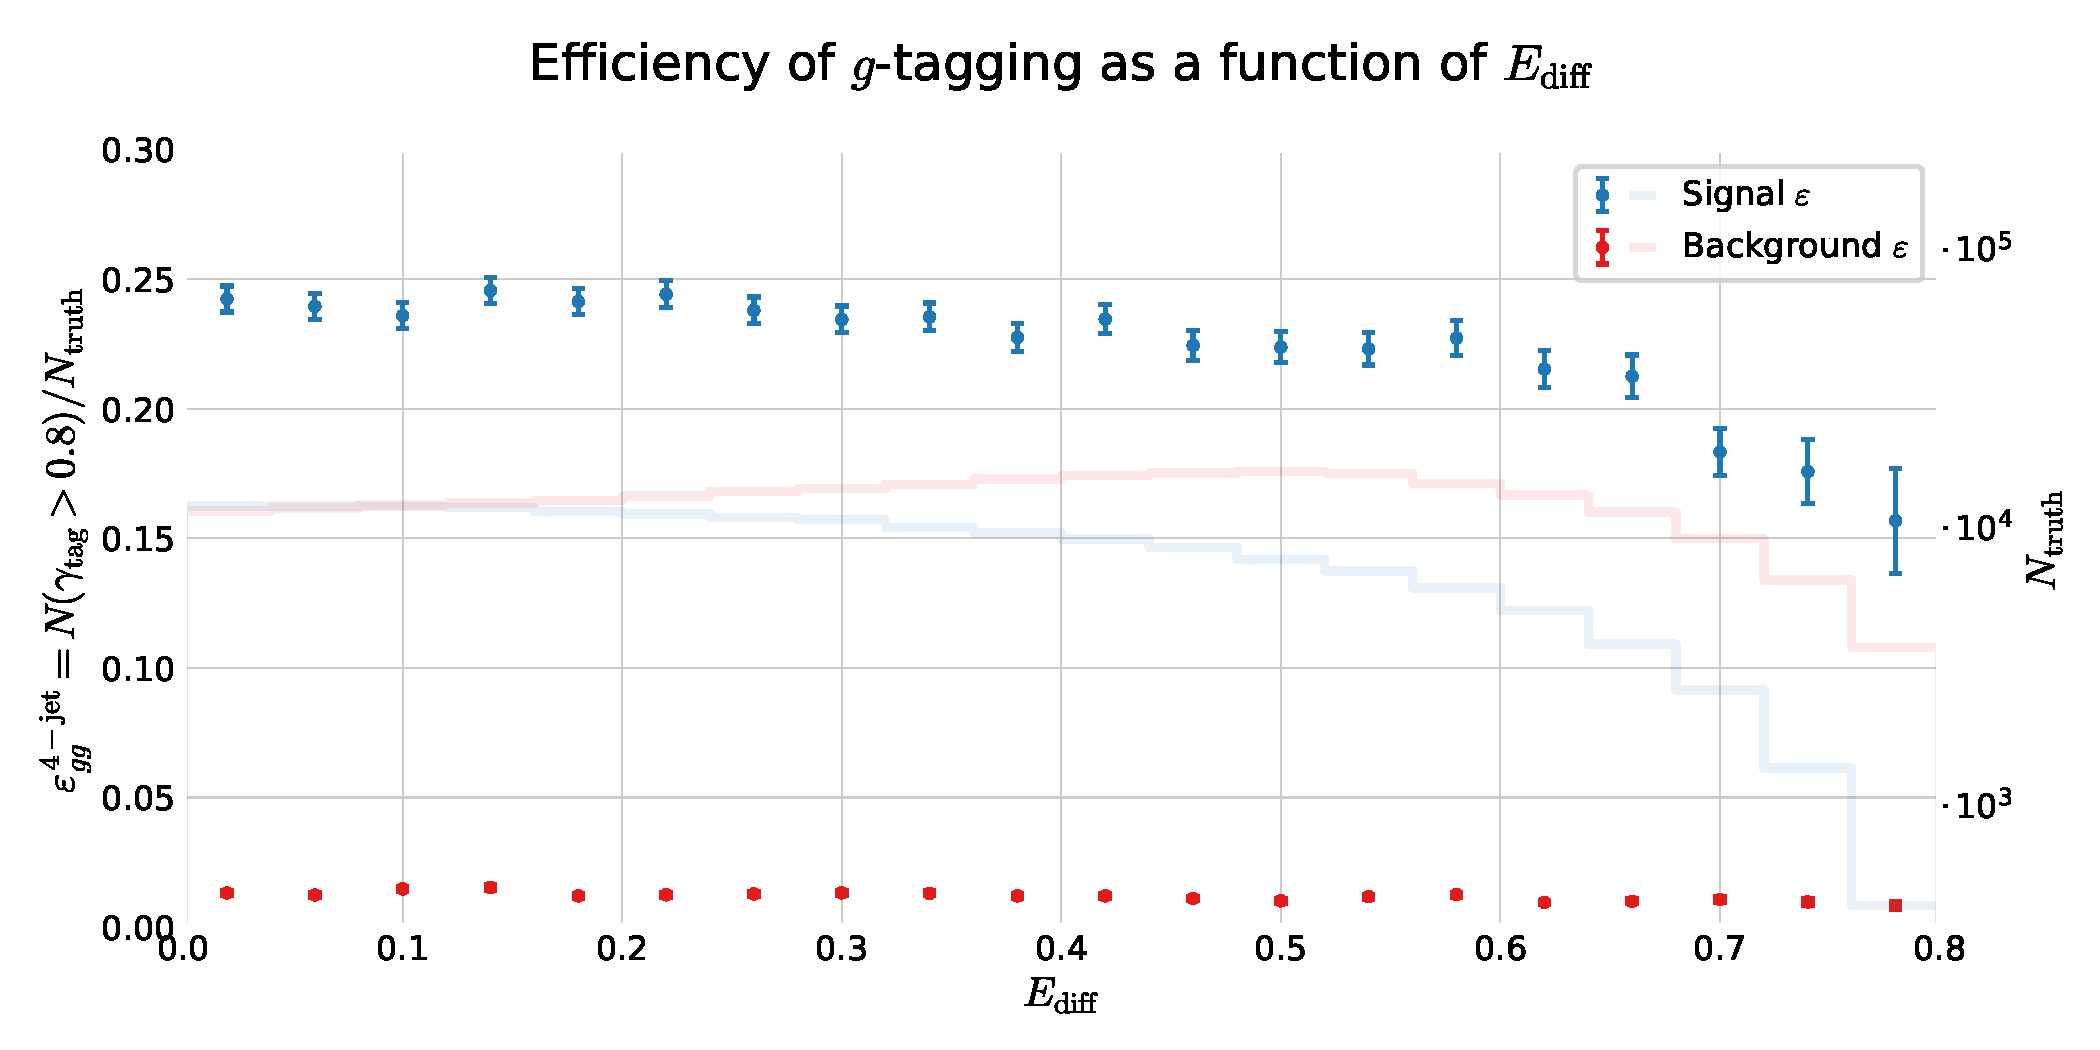
\includegraphics[width=0.95\textwidth, trim=0 0 0 40, clip, page=1]{figures/quarks/efficiency_events-down_sample=1.00-ML_vars=vertex-selection=b-ejet_min=4-n_iter_RS_lgb=99-n_iter_RS_xgb=9-cdot_cut=0.90-version=19-njet=4.pdf}
  \caption[g-Tagging efficiency for 4-jet events in MC as a function of normalized gluon gluon jet energy difference]
          {Efficiency of the g-tags for 4-jet events as a function of normalized gluon gluon jet energy difference in Monte Carlo. The efficiency is measured as the number of events with a g-tag higher than 0.8 ($\gamma > 0.8$) out of the total number and the normalized gluon gluon jet energy difference $A$ is $A=\frac{E_{g_\mathrm{max}}-E_{g_\mathrm{min}}}{E_{g_\mathrm{max}}+E_{g_\mathrm{min}}}$ where $E_{g_\mathrm{max}}$ ($E_{g_\mathrm{min}}$) refers to the energy of the gluon with the highest (lowest) energy. The efficiency is plotted for \textcolor{blue}{signal events} according to MC Truth in blue and \textcolor{red}{background events} according to MC Truth in red.
          } 
  \label{fig:q:effiency_gtag_E_diff}
\end{figure}


\begin{figure}
  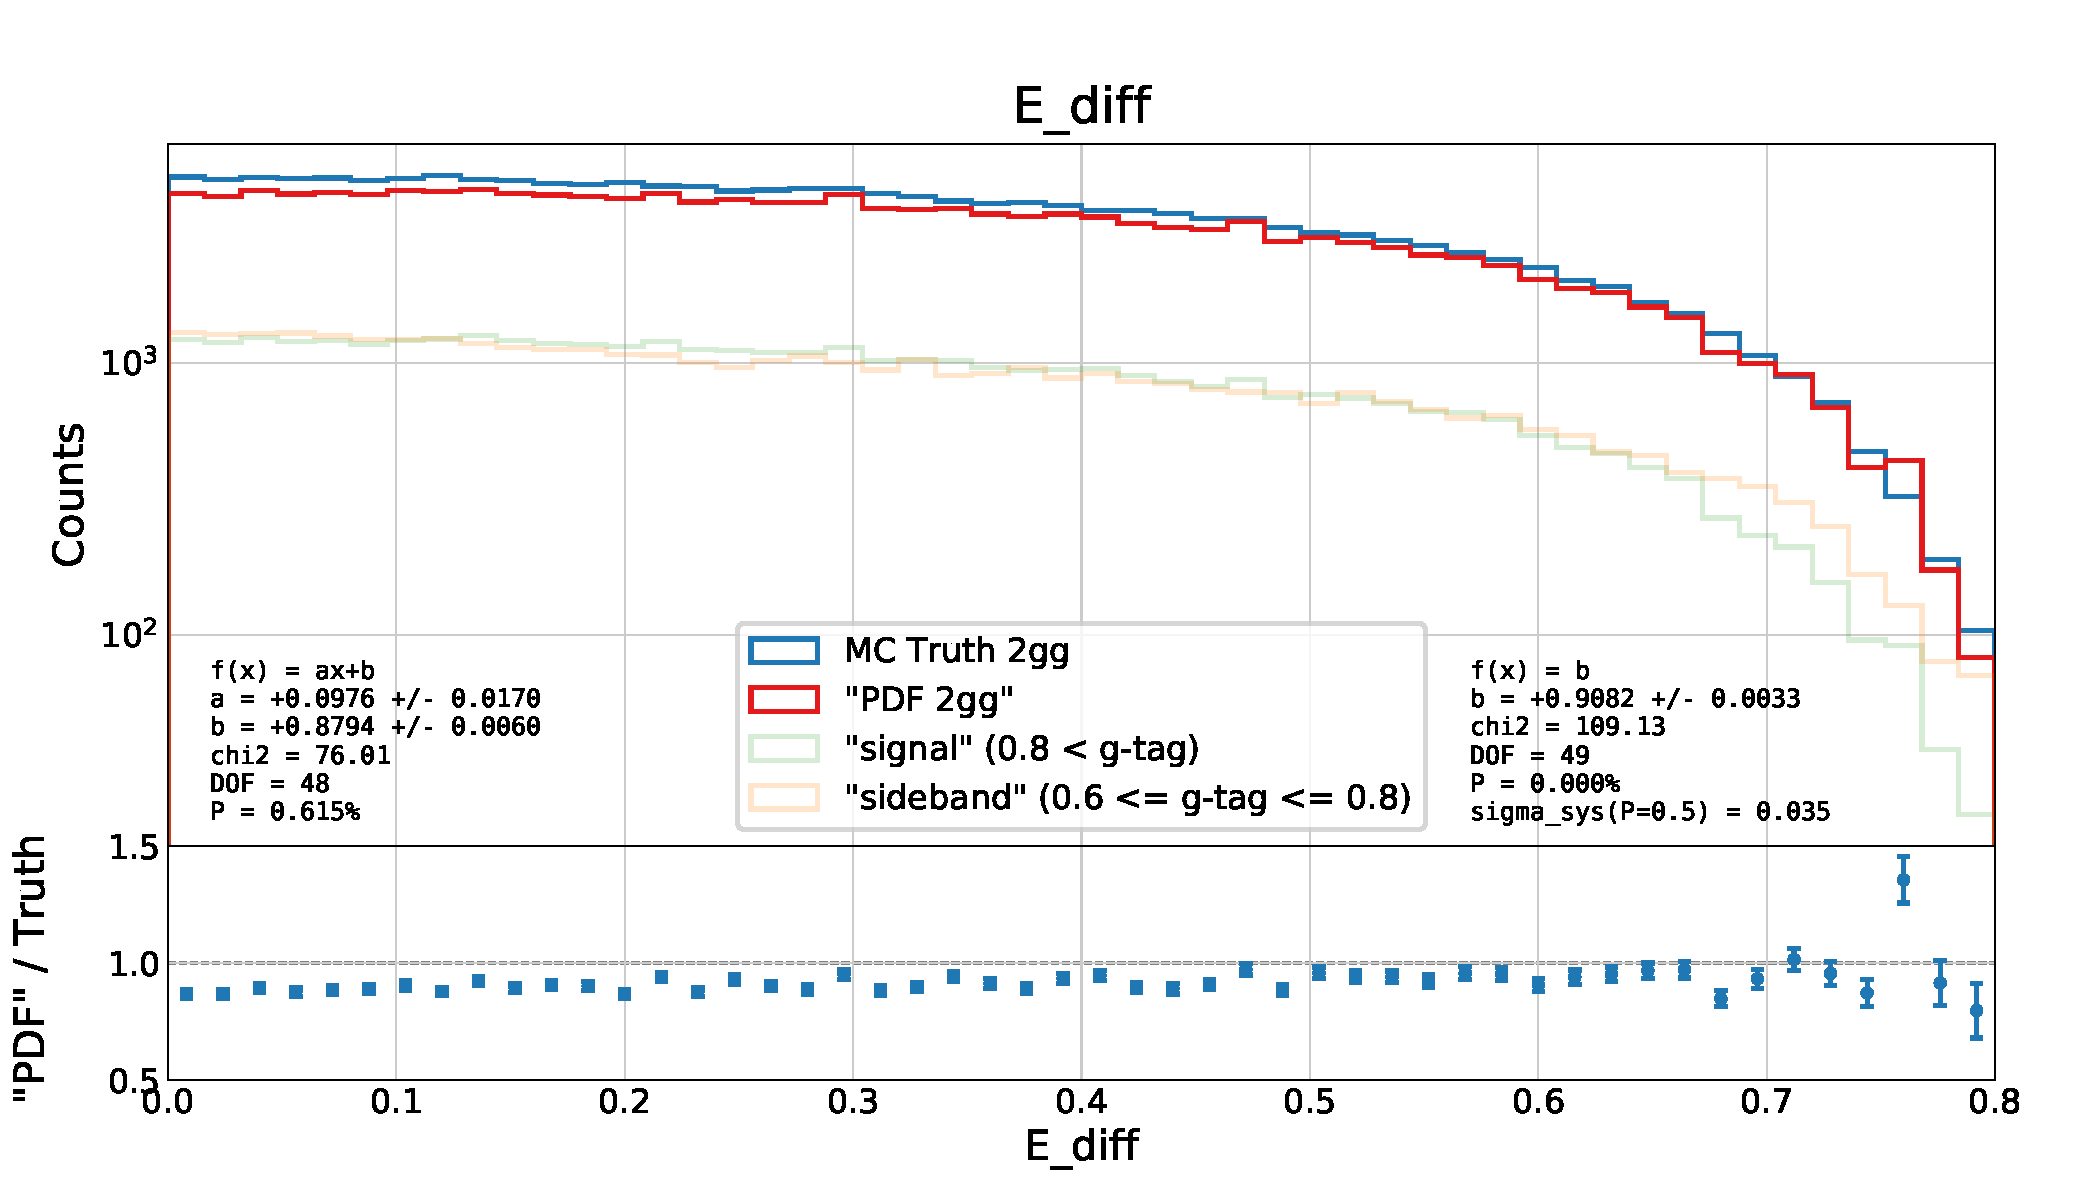
\includegraphics[width=0.95\textwidth, trim=0 0 0 65, clip, page=1]{figures/quarks/gtag-closure_test-down_sample=1.00-ML_vars=vertex-selection=b-ejet_min=4-n_iter_RS_lgb=99-n_iter_RS_xgb=9-cdot_cut=0.90-version=19-njet=3.pdf}
  \caption[Closure plot between MC Truth and the corrected g-tagging model in 4-jet events for the normalized gluon gluon jet energy difference]
          {Closure plot between MC Truth and the corrected g-tagging model in 4-jet events for the normalized gluon gluon jet energy difference. The corrected g-taggingg model is described in further detail in section XXX \TODO. In the top part of the plot the \textcolor{blue}{MC Truth} is shown in blue, the \textcolor{red}{corrected g-tagging model} \code{"PDF 2gg"} in red, the \textcolor{green}{g-signal distribution} in semi-transparent green and the \textcolor{orange}{g-sideband distribution} in semi-transparent orange. In the bottom part of the plot the ratio between MC Truth and the output of the corrected g-tagging model is shown. The normalized gluon gluon jet energy difference $A$ is $A=\frac{E_{g_\mathrm{max}}-E_{g_\mathrm{min}}}{E_{g_\mathrm{max}}+E_{g_\mathrm{min}}}$ where $E_{g_\mathrm{max}}$ ($E_{g_\mathrm{min}}$) refers to the energy of the gluon with the highest (lowest) energy.
          } 
  \label{fig:q:closure_E_diff}
\end{figure}


\begin{figure}
  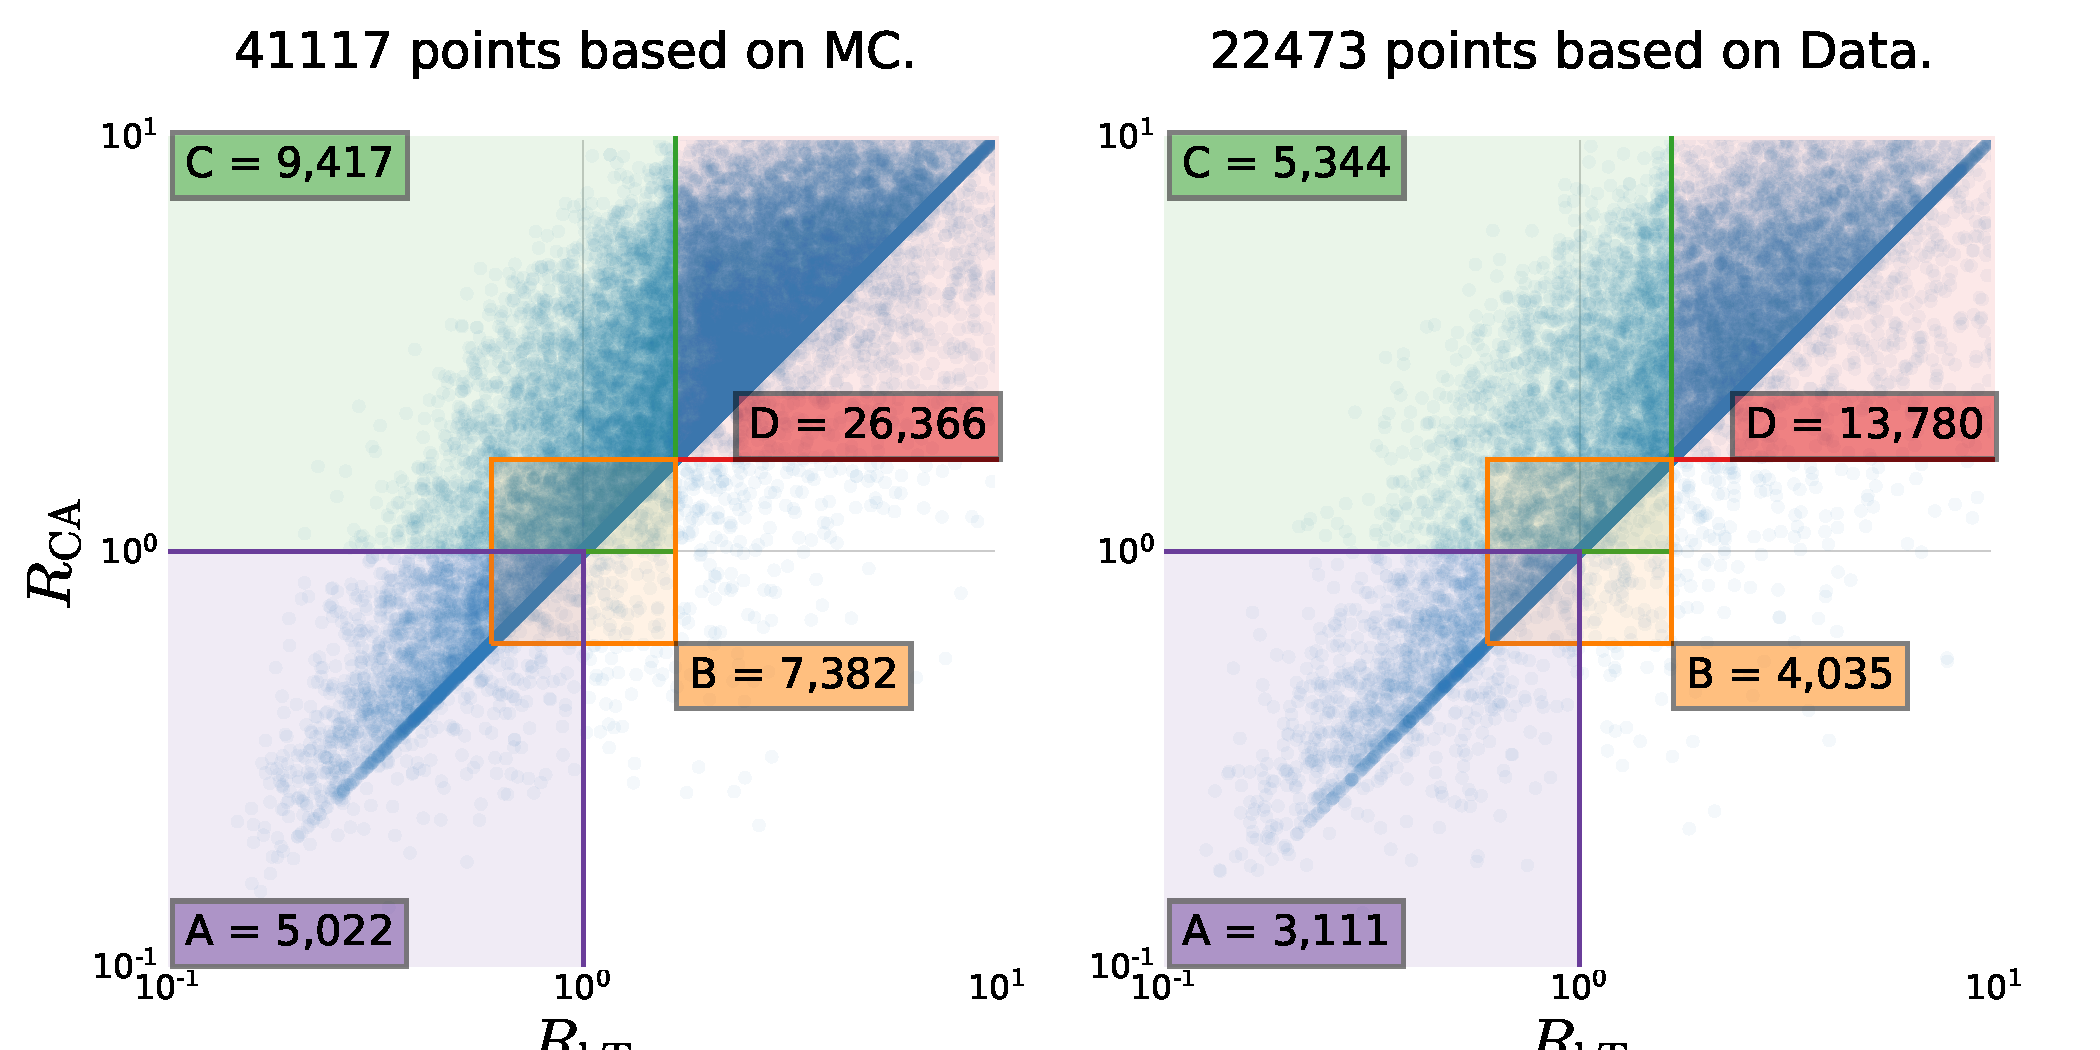
\includegraphics[width=0.95\textwidth, trim=0 0 0 118, clip, page=1]{figures/quarks/gtag-R_kt_CA_overview-down_sample=1.00-ML_vars=vertex-selection=b-ejet_min=4-n_iter_RS_lgb=99-n_iter_RS_xgb=9-cdot_cut=0.90-version=19-njet=4}
  \caption[R kt CA overview  XXX \TODO]
          {R kt CA overview XXX \TODO
          } 
  \label{fig:q:R_kt_CA_overview}
\end{figure}

\begin{figure}
  \includegraphics[width=0.95\textwidth, trim=0 0 0 30, clip, page=2]{figures/quarks/gtag-R_kt_CA_overview-down_sample=1.00-ML_vars=vertex-selection=b-ejet_min=4-n_iter_RS_lgb=99-n_iter_RS_xgb=9-cdot_cut=0.90-version=19-njet=4}
  \caption[R kt CA cut region A  XXX \TODO]
          {R kt CA cut region A XXX \TODO
          } 
  \label{fig:q:R_kt_CA_cut_A}
\end{figure}
